%%% File encoding: UTF-8
%% äöüÄÖÜß  <-- no German Umlauts here? Use an UTF-8 compatible editor!

%%% Magic comments for setting the correct parameters in compatible IDEs
% !TeX encoding = utf8
% !TeX program = pdflatex
% !TeX spellcheck = en_US
% !BIB program = biber




\documentclass[master,english, twoside, openright]{hgbthesis}
% Permissible options in [..]:
%   Type of work: diploma, master (default), bachelor, internship
%   Main language: german, english (default)
%%%----------------------------------------------------------




\RequirePackage[utf8]{inputenc}		% Remove when using lualatex or xelatex entfernen!

\graphicspath{{images/}}    % location of images and graphics
\logofile{unib.png}				% logo file = images/logo.pdf (use \logofile{} for no logo)
\bibliography{references}  	% name of bibliography file (references.bib)

%%%----------------------------------------------------------
% Title page entries
%%%----------------------------------------------------------

%%% Entries for ALL types of work: --------------------------
\title{Development of a Visual Voice Activity Detection}
\author{Adrian David Lubitz}
\programname{Systems Engineering}
\placeofstudy{University of Bremen}
\dateofsubmission{2019}{10}{12}	% {YYYY}{MM}{DD}

%%% Entries for Bachelor theses only: -----------------------
\thesisnumber{XXXXXXXXXX-A}   %e.g. 1310238045-A
% (Stud-ID, A = 1st Bachelor thesis)
\semester{Fall Semester 2018} 	% Fall/Spring Semester YYYY
\coursetitle{}
\advisor{Matias Valdenegro Toro}


%%% Restricted publication license instead of CC (master only):
%\strictlicense

%%%----------------------------------------------------------
\begin{document}

%%%----------------------------------------------------------

%%%----------------------------------------------------------
\frontmatter							% title part (roman page numbers)
%%%----------------------------------------------------------

\maketitle
\setcounter{secnumdepth}{3}

\chapter{Acknowledgment}
I would like to express my special appreciation and thanks to my supervisor \textbf{Dr. Matias Alejandro Valdenegro Toro} who guided the scientific process throughout the research for this thesis.
Furthermore he helped my with his great experience in Deep Learning to get a profound understanding of the topic.

Additionally I want to thank my mentor \textbf{Marc Fiedler}, CEO of \emph{Blackout Technologies}, for his kind, motivating and encouraging way of making the thesis possible in cooperation with Blackout Technologies. I want to thank the whole team at Blackout Technologies for their precious support while I was working on my thesis.

A special thanks goes to the \textbf{Deutsches Forschungszentrum für Künstliche Intelligenz (DFKI)} for arousing my interest in Robotics and Artificial Intelligence with their outstanding courses in this area.
Furthermore I want to thank the DFKI for the access to their GPU-Cluster which enabled me to train all the different models in a reasonable time.

Finally I want to thank my family, my girlfriend and all teachers who supported me on my way throughout life to achieve my goals and sustain my curiosity and joy in learning.






 	% preface is optional
\chapter{Abstract}
Technology is integrating more and more into the life of the modern man. A very important
question is how are people interacting with technology.
The human brain does not react emotionally to artificial objects like computers and
mobile phones. However, the human brain reacts strongly to human appearances like
the shape of the human body or faces. Therefore humanoid robots are the most
natural way for human-machine interaction, because of the human-like appearance.
It is obvious that not only the physical appearance needs to be human-like, also the psychological concepts of interaction need to be implemented.
Modern social robots like Pepper from SoftBank Robotics Group Corp. already come with a handful of cognitive features like stimuli reaction or gaze detection.

To make human-machine interaction more natural further cognitive features need to be implemented. 
For this purpose, this proposed master thesis will deal with the problem of a Visual Voice Activity Detection (VVAD), which can detect whether a person is speaking to a robot or not, given the visual input of the robot's camera.
This cognitive feature can solve the problem of
speaker identification in situations, where it is not trivial like crowded areas and when more than one person is in the robot's field of view.

To implement the described VVAD an approach based on a recurrent neural network, to model the time dependencies in the input data,
and convolutional layers, to learn features from pixels, is presented.
Most classic approaches to VVAD unfold to lip motion detection which yields in a high false positive rate because humans make arbitrary lip motion even when not speaking.
To deal with this the network is trained on a slightly adjusted version of the LRS3 dataset. 
The LRS3 dataset contains more than 100.000 video sequences of people speaking. 
Faces will be extracted from the video sequences using correlation based tracking and face detection. 
The evaluation compares two different approaches.
One extracts facial features from the face detection and uses them as the input vector for the network while the other is End-To-End-Learning which uses the whole image as an input vector of pixels. 
These two approaches can again be gradually divided by the area used as input. 
Either the whole face will be used or only the lips.
We find that for this problem, an LTSM-FCN with images of the whole face works best with 92\% accuracy on the VVAD dataset.

\chapter{Kurzfassung}
\begin{german}
Technologie verschmilzt mehr und mehr mit dem Leben der Menschen. 
Eine der wichtigsten Fragen hierbei wird sein, wie Menschen mit Technologie interagieren.
Das menschliche Gehirn zeigt nur sehr geringe emotionale Reaktionen auf künstliche Objekte, wie Computer und Handys.
Anders verhält es sich bei Dingen, die menschlich wirken. Dinge die einem Gesicht oder dem menschliche Körper ähneln, können eine stärkere emotionale Reaktion herbeiführen.
Auf diese Grundlage stützt sich die These, dass humanoide Roboter das natürlichste Mittel zur Interaktion mit Technologie darstellen.
Hierbei ist es einleuchtend, dass nicht nur die physische Form menschlich sein muss, sondern auch kognitive Konzepte greifen müssen, um ein menschenähnliches Verhalten zu simulieren.
Moderne soziale Roboter, wie Pepper von SoftBank Robotics Group Corp. bringen bereits einige dieser kognitiven Fähigkeiten mit, wie zum Beispiel die Reaktion auf auditive und taktile Stimuli oder Blickkontakterkennung.
Um die Mensch-Maschine-Kommunikation natürlicher zu machen, müssen weitere kognitive Fähigkeiten entwickelt werden.
Im Rahmen dieser Masterarbeit wird eine visuelle Sprachaktivitätserkennung entwickelt, welche es einem Roboter ermöglicht ausschließlich anhand der Kameradaten zu erkennen, ob eine Person spricht oder nicht.
Diese kognitive Fähigkeit ermöglicht es auch in lauten und überfüllten Umgebungen oder Situationen mit mehrere Personen im Blickfeld des Roboters eine sichere Prognose darüber zu stellen, welche Person mit dem Roboter spricht.
Um die beschriebene visuelle Sprachaktivitätserkennung zu implementieren wird ein Ansatz auf Basis von Rekurrenten Neuronalen Netzen, um die zeitliche Abhängigkeit der Daten zu modellieren, sowie Convolutionalen Neuronalen Netzen, um die örtliche Abhängigkeit zu modellieren, verwendet.
Die meisten klassischen Ansätze setzten auf die Erkennung von Lippenbewegungen, was allerdings zu vielen fälschlicherweise positiv klassifizierten Beispielen führt, weil der Mensch in Phasen, in denen nicht gesprochen wird unwillkürliche Lippenbewegungen durchführen kann.
Um diese Falschklassifizierungen zu umgehen, wird eine angepasste Version des LRS3 Datensatzes verwendet.
Der LRS3 Datensatz besteht aus über 100.000 Videosequenzen, die Menschen beim Sprechen zeigen.
Aus diesen werden Sequenzen, die Gesichter zeigen, mittels korrelationsbasiertem Tracking, sowie Gesichtserkennung extrahiert.
In der Evaluation werden zwei verschiedene Ansätze untersucht.
Ersterer verwendet Merkmale aus der Gesichtserkennung, um anhand dieser Daten zu lernen, während der zweite Ansatz ein Ende-zu-Ende Lernansatz ist, welcher direkt auf den Pixelwerten lernt.
Diese beiden Ansätze können noch einmal graduell anhand des Bereiches unterteilt werden, welcher für das Lernen verwendet wird.
Hierbei wird der Fokus entweder auf das gesamte Gesicht oder nur auf  die Lippen gelegt.  
Mit einem LSTM-FCN trainert auf Bildern von Gesichtern wurde eine Genauigkeit von 92\% für den VVAD Datensatz erreicht.
\end{german}

\tableofcontents



%%%----------------------------------------------------------
\mainmatter          			% main part (arabic page numbers)
%%%----------------------------------------------------------

%!TeX spellcheck = en-US
\chapter{Introduction}\label{cha:Introduction}
Technology is integrating more and more into the life of the modern man. A very important
question is how are people interacting with technology.
The human brain does not react emotionally to artificial objects like computers and
mobile phones. However, the human brain reacts strongly to human appearances like
the shape of the human body or faces. Therefore humanoid robots are the most
natural way for human-machine interaction, because of the human-like appearance.
This hypothesis is strongly supported by Takayuki Kanda and Hiroshi Ishiguro in \cite{kanda2017human}.
They see Social Robots as a part of the future society as shown in figure \ref{fig:socialRobotsFuture}.
\begin{figure}
  \centering
  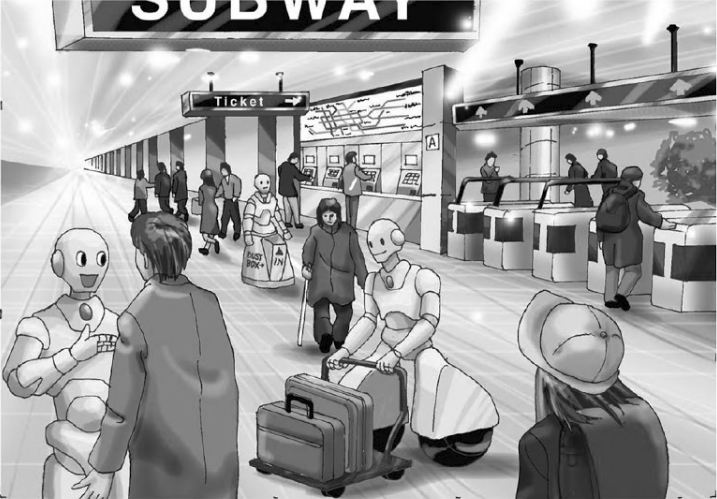
\includegraphics[width=.6\textwidth]{socialRobotsFuture.png}
  \caption{Social Robots in the future society \cite{kanda2017human}}
  \label{fig:socialRobotsFuture}
\end{figure}
Takayuki Kanda and Hiroshi Ishiguro also define the following three issues which
need to be solved to bring social robots effectively and safely to the everyday life:
\begin{itemize}
  \item [a.] Sensor network for tracking robots and people
  \item [b.] Development of humanoids that can work in the daily environment.
  \item [c.] Development of functions for interactions with people.
\end{itemize}
This thesis is located in the field \texttt{c}, as we try to implement a Visual Voice Activity Detection (VVAD) which detects whether a person is speaking to a robot or not, given the visual input of the robot's camera. The detailed description of the problem
setting is given in Section \ref{sec:problem}.


\section{Motivation}\label{sec:motivation}
In this Section we want to present why a VVAD is an important cognitive feature in a Human-Robot Interaction(HRI).
As we want Robots to integrate seamlessly into our society, Human-Robot Interaction needs to be as close as possible to Human-Human Interaction(HHI). To achieve this goal we need to understand how humans communicate.
In specific we need to know how humans start a conversation.
There is one main concept when it comes to starting an interaction, which is deeply encoded in our DNA, as it is used by newborns and even animals follow this concept. To start a interaction of any kind one needs to increase the attention of the other. In HHI an increased attention comes mainly from the following stimuli:
\begin{itemize}
  \item {1.} auditory stimuli
  \item {2.} tactile stimuli
  \item {3.} visual stimuli
\end{itemize}
In the context of a conversation all the above stimuli can represent a direct starting point to a conversation.
For auditory stimuli a direct starting point can be a name or a word socially known to increase attention
like \emph{hey} in the English language. Calling someones name works like a directed message to someone, while words like \emph{hey} work like a broadcast to everyone in the surrounding. The concept of using names as a trigger phrase for virtual assistant systems is implemented in well known assistants like the Amazon Alexa, the Google Assistant or Apples Siri.

A tactile stimulus gives direct attention because the human body is very sensitive to tactile stimuli in a way that every individual has it's own private space. A tactile stimulus is invading a humans personal space and is therefore triggering an increase in attention. Meaning when you touch someone and say something directly afterwards the touched person can directly process the message, because of the increased attention.

For visual stimuli gaze and eye contact have been studied for decades, because they have such a special role in HHI. As Michael Argyle and Janet Dean stated in \cite{ARGYLE1965} gaze has a huge influence on the personal space and therefore also increases the attention. Meaning if eye contact is established and one of the two parties speaks it works like a directed message.


As the hypothesis of Takayuki Kanda and Hiroshi Ishiguro is that humans will react more naturally to human-like robots, it is obvious that not only the physical appearance needs to be human-like, also the psychological concepts of interaction need to be implemented.

For the purpose of this thesis we want to enhance the implementation of a Pepper Robot from SoftBank Robotics Group Corp.(a detailed description of the robot can be seen in Appendix \ref{sec:pepper}).\footnote{All further mentions of \emph{the robot} refer to the Pepper Robot}
The robot already is able to react to the described stimuli. Nevertheless there is a gap after that.
Assuming someone is establishing eye contact with the robot.
Which will result in an increase of the robots attention, meaning he will start listening.
But the problem here is that the robot does not have the capability to detect if the person, eye contact is established with, is speaking.
The robot may respond to something someone else in the surrounding was saying, which will confuse the person, eye contact is established with, and result in a non natural way of communication.
To solve this problem we want to develop a VVAD which detects whether a person is speaking to a robot or not, given the visual input of the robot's camera. Thus the robot can decide whether to listen if the person is speaking to it or to proactively act on the invasion of it's personal space if the person is just starring at the robot.
We hope that this social skill will improve the quality of HRI in a way that communicating with a robot feels more natural.




\section{Problem Setting}\label{sec:problem}

As stated before this thesis deals with the implementation of a VVAD which detects whether a person is speaking to a robot or not, given the visual input of the robot's camera.
We consider an open world setting in which people start an interaction with the robot whenever they want and it can also occur that people are talking near the robot without talking directly to the robot.
In such an environment the robot should be able to react on a visual stimulus (described in Section \ref{sec:motivation}) as natural as possible.
The algorithm to classify whether a person is just starring at the robot or is speaking to the robot will be performed solely on video data from the camera of the robots head. This seems to be unnecessary few input on first sight, as the robot provides a lot more useful information, like audio input and even echo location. But with a closer look to the described cognitive feature of detecting an invasion of personal space on the basis of visual stimuli, it is only logical to reduce the input to only visual information. A fusion of different cognitive features could happen on a higher level of cognition.
As described in Section \ref{sec:motivation} we use a Pepper Robot as the target platform. Pepper provides video data in a maximum resolution of 2592x1944 pixels at a framerate of 1 fps or with a maximum framerate of 30 fps with a resolution of 640x480 pixels(for further details of the given Hardware see Appendix \ref{sec:pepper} and \cite{Pepper2018}).


\section{Approach}\label{sec:approach}
%(taking the 30 fps)
%training data
%RNN
%different modeling approaches
% 1. Feature reduction(relative postion?)
%  1.1 only mouth features
%  1.2 whole face features
% 2. Direct Learning(name?)
%  2.1 only mouth image
%  2.2 whole face image
In this Section we will describe the approach to develop a VVAD which detects whether a person is speaking to a robot or not, given the visual input of the robot's camera. This goes from the training data over the learning algorithm to the evaluation.
\subsection{Training data}\label{ssec:data}
To train our classifier we need a dataset which has labeled video data. As we try to solve a binary classification problem the data needs to have two labels. In our case these would be \emph{speaking} as the positive class and \emph{not speaking} as the negative class on every sample of the dataset. We also need a Region of Interest (ROI) on every image. So we end up with samples, that are labeled video sequences of faces either \emph{speaking} or \emph{not speaking}.
The University of Oxford developed three datasets(LRW, LRS2, LRS3) for lipreading in cooperation with the BBC and TED \cite{Chung16}, \cite{Chung17},\cite{Chung18}. These need to be slightly adjusted to the purpose of the thesis. The video data is labeled with words and the corresponding timestamps. It also provides a face bounding box for every frame.
The positive class can be easily extracted from this datasets, as we know which frames correspond to speech.
The negative class needs to be extracted from the phases where the person is not speaking, which can be slightly more challenging because the phases are not stored in the dataset's labels. As we know there is no speech in those phases we follow the given face from the ROI to construct a negative sample if the number of frames is over a given threshold.

\subsection{Learning algorithm}\label{ssec:algorithm}
To choose a good fit for the learning algorithm it is important to exploit the knowledge of the underlying data. In the case of a VVAD, we are dealing with sequences of video frames.
%Following \cite{Zhengzheng2010} a sequence can be described as follows:
%\begin{itemize}
%\item[•] Given an alphabet of symbols  $\left\lbrace E_1, E_2, E_3, ..., E_n \right\rbrace$, a
%\emph{simple symbolic sequence} is an ordered list of the symbols
%from the alphabet. For example, a DNA sequence
%is composed of four animo acid A, C, G, T and a DNA
%segment, such as ACCCCCGT, is a simple symbolic
%sequence.
%\item[•] A \emph{complex symbolic sequence} is an ordered list of vectors.
%Each vector is a subset of the alphabet \cite{Lesh99}. For
%example, for a sequence of items bought by a customer
%over one year, treating each transaction as a
%vector, a sequence can be $\left\langle (milk, bread)(milk, egg)\cdots(potatos, cheese, coke)\right\rangle$.
%\item[•] A \emph{simple time series} is a sequence of real values ordered
%in timestamp ascending order. For example, $\left\langle(t_1, 0.1)(t_2, 0.3)\cdots(t_n, 0.3)\right\rangle$
%is a simple time series recording the data from time
%stamp $t_1$ to $t_n$.
%\item[•] A \emph{multivariate time series} is a sequence of numerical
%vectors. For example,
%
%$\left\langle (t_1,\left\langle 0.1, 0.3, 05\right\rangle )(t_2,\left\langle 0.3, 0.9, 0.8\right\rangle )\cdots(t_n,\left\langle 0.3, 0.9, 0.4\right\rangle )\right\rangle $
%is a multivariate time series.
%\item[•] In the above, the data types of the events are simple.
%In some applications, the data type of events can be arbitrarily
%complicated. For example, in a patient record
%data set (\url{http://www.informsdmcontest2009.org/}),
%each patient is represented by a longitudinal sequence
%of hospital visits. Each visit is an event and is described
%by multiple numerical measurements, categorical
%fields and text descriptions. A \emph{complex event sequence}
%refers to the general form of sequences.
%\end{itemize}
As described in Section \ref{ssec:data} every sample is annotated with a positive (\emph{speaking}) or a negative (\emph{not speaking}) label $y$ and is described by a  ROI as a face bounding box from which we can extract a vector of features(these can be the pixels directly or features from the face detection) $\mathbf{x} = \left\langle x_{0}, x_{1}, \cdots , x_{n-1}, x_{n} \right\rangle$. What we want is a classifier that maps a sequence of those frames to a class.
\begin{equation}\label{eq:classifier}
f: \left\langle \mathbf{x}_{t}, \mathbf{x}_{t-1}, \cdots, \mathbf{x}_{t-k} \right\rangle \rightarrow y_{t} \quad |\ y \in \left\lbrace0,1\right\rbrace,\ k \in \mathbb{N}\ |\ 0<k\leq t
\end{equation}
This classifier uses a temporal sliding window, to always perform the classification on the last $k$ frames. The hyperparameter $k$ needs to be chosen  small enough to make the classification fast enough, but needs to be chosen big enough to secure accuracy.
For $\mathbf{x}$ we will evaluate four different approaches.
These can be split in $2 \times 2$ categories. The first categories are \emph{Focus on facial features} or \emph{End-to-End Learning}.
The second categories are \emph{only mouth} or \emph{whole face}.
This will end up in the following four models, which should be tested against each other:
\begin{itemize}
  \item Focus on facial features
  \begin{itemize}
  	\item only mouth features
  	\item whole face features
  \end{itemize}
  \item End-to-End Learning
  \begin{itemize}
  	\item only mouth image
  	\item whole face image
  \end{itemize}
\end{itemize}
For the facial features we want to use dlib's\cite{Dlib} pretrained Convolutional Neural Network (CNN) for face shape detection which gives 68 features for a face including 20 features for the mouth.
Independent of which model we use, we will need to apply some kind of normalization to the scale, rotation and translation of the features. The face or the mouth can appear in any translation, rotation and scale in the dataset, with the normalization we make sure that we concentrate on the important features of the image. Otherwise it could happen, that the classification is based on the position of the face in the image, which is obviously not correct.
As we want to know the label for a ongoing sequence as fast as possible it is considered to be a problem of early classification of time series
data \cite{Xing2011}. As described earlier we use a fixed size temporal sliding window to solve this issue.
Our approach to solve the classification problem is a Long Short Term Memory (LSTM) Fully Convolutional Network (FCN).
As shown in \cite{Fazle18} \cite{Fazle17} Recurrent Neural Networks (RNNs) and in specific LSTM-FCNs are the state of the art method for Time Series Classification.

\subsection{Evaluation}\label{ssec:evaluation}
To evaluate the classification we will use a dedicated test set created with the extraction of the samples from the LRS3 dataset. 
For this test set a human accuracy level test is conducted to evaluate the results from a test on that specific test set. 
Furthermore the human accuracy level test can give information about the quality of the constructed dataset.
The evaluation is performed on the described four different learning approaches in terms of the input features described in Section \ref{ssec:algorithm}. 

\section{Related Works}\label{sec:relatedWorks}
The classic approach to solve Visual Voice Activity Detection is to detect lip motion.
This approach is taken by F. Luthon and  M. Liévin in \citep{Luthon1998}. They try to model the motion of the mouth in a sequence of color images with Markov Random Fields. For the lip detection they analyze the images in the \emph{HIS ( Hue,
Intensity, Saturation )} color space, with extracting \emph{close-to-red-hue prevailing regions} this leads to a robust lightening independent lip detection.
A different approach was taken by Spyridon Siatras, Nikos Nikolaidis, and Ioannis Pitas in \cite{Siatras2006}. They try to convert the problem of lip motion detection into a signal detection problem. They measure the intensity of pixels of the mouth region and classify with a threshold, since they argue that frames with an open mouth have a essentially higher number of pixels with low intensity.
In \citep{Bendris2010} Meriem Bendris, Delphine Charlet and Gérard Chollet propose a method,
which measures the probability of voice activity with the optical flow of pixels in the mouth region. In this paper the drawback of lip motion detection based approaches is already discussed.
As shown in Figure \ref{fig:errorDetection} the problem is that people move their lips from time to time although they are not speaking.

\begin{figure}
\centering
  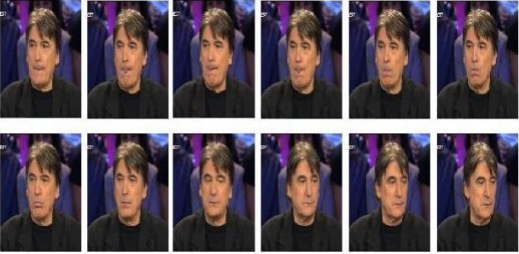
\includegraphics[width=.75\textwidth]{error_detection.png}
  \caption{Example of error detection - Person is classified as
having a mouth activity, however does not speak \cite{Bendris2010}}
  \label{fig:errorDetection}
\end{figure}

This issue is tackled by Foteini Patrona, Alexandros Iosifidis et al. \cite{Patrona2016}.
They use a Space Time Interest Point(STIP) or the Dense Trajectory-
based facial video representation to train a Single Hidden Layer Feedforward Neural Network.
The features are generated from the CUAVE dataset \cite{Patterson2002}.
This erases the implicit assumption (of the approaches above) that lip motion equals voice activity.
A more robust approach, which uses Centroid Distance Features of normalized lip shape to train a LSTM Recurrent Neural Network is proposed by Zaw Htet Aung and Panrasee Ritthipravat in \cite{Aung2015}. This method shows a classification accuracy up to 98\% on a relatively small dataset.
In conclusion all of the mentioned methods use some kind of face detection and some also use mechanics to track the face. This is needed if there is more than one face in the image.
From the facial images features are created in different ways. From that point the approaches divide into two branches.
The first and naive approach is to assume that lip motion equals speech. This is obviously not always the case, which is why the later approaches do not rely on this hypothesis.
The latter approach uses learning algorithms to learn the real mapping between facial images and the speech/no speech. This approach is strongly relying on a balanced dataset to learn a good performing model.

\section{Software}
\label{sec:software}
In larger projects, independent if its software, hardware or even something else, it makes sense to
take advantage of the knowledge of others.
In terms of software this can be very easy, because the Internet is full of libraries, that provide solutions for various problems.
The few used to implement the VVAD are presented in the following.
\subsection{Keras}
To design the Deep Neural Networks used to make the prediction for the VVAD \emph{Keras}\cite{Keras} is used.
Keras is a python library which provides a high-level API(Application Programming Interface) for Artificial Neural Networks. It is designed to run on top of TensorFlow, CNTK or Theano and abstracts their implementation to a easy to use API for Deep Learning. 
It supports computation on CPU and GPU.
\subsection{NumPy}
\emph{NumPy}\cite{NumPy} is the go to library for scientific computations in python.
It provides powerful computation in linear algebra due to its C++ implementation. 
NumPy is used to transform all data into the shape needed by Keras and to produce meaningful visualizations of the data.  
\subsection{Dlib}
\emph{Dlib}\cite{Dlib} is a C++ library with very good python bindings which provides a lot of machine learning and image processing algorithms.
Dlib's face detection, tracking and facial landmark detection is used to construct the VVAD dataset from the LRS3 dataset.
\subsection{OpenCV}
Similar to Dlib, \emph{OpenCV}\cite{OpenCV} is a C++ implementation with strong python bindings. 
OpenCV provides a great variety of algorithms from the field of computer vision.
It is used for its very efficient basic operations on images, like loading, resizing and transformation to different color spaces.
\subsection{Express}
\emph{Express}\cite{EXPRESS} is a NodeJS library which provides a high-level API for the design of web apps.
Express is used for the Human Accuracy Level Test described in Section \ref{ssec:VVADHACL}.
\subsection{MongoDB}
\emph{MongoDB}\cite{MONGO} is a cross-platform document-oriented NoSQL database, which is used to store the classifications made in the Human Accuracy Level Test.

\section{Contribution}
In this thesis the problem of VVAD is defined and a large scale dataset called the \emph{VVAD dataset} (see Section \ref{sec:vvadData}) is constructed for this purpose.
The results obtained in this thesis using the proposed different approaches define the state of the art for VVAD problem.
Table \ref{tb:accuracies} shows an overview of the accuracies reached by the different approaches.


%\section{Time table}
%
%\begin{ganttchart}[vgrid={draw=none, dotted}]{1}{24}
%\gantttitle{Weeks}{24} \\
%\gantttitlelist{1,...,24}{1} \\
%\ganttbar{Literature Research}{1}{5} \\
%\ganttbar{Data acquisition}{3}{7} \\
%\ganttbar{Implementing models}{7}{16} \\
%\ganttbar{Tuning models}{16}{19} \\
%\ganttbar{Evaluation}{19}{23} \\
%\ganttbar{Writing thesis}{3}{24}
%\end{ganttchart}


%\begin{ganttchart}[vgrid={draw=none, dotted}]{1}{24}
%\gantttitle{Weeks}{24} \\
%\gantttitlelist{1,...,24}{1} \\
%\ganttbar{Literature Research}{1}{5} \\
%\ganttbar{Data acquisition}{3}{7} \\
%\ganttbar{Implementing models}{7}{16} \\
%\ganttbar{Tuning models}{16}{19} \\
%\ganttbar{Evaluation}{19}{23} \\
%\ganttbar{Writing thesis}{3}{24}
%\end{ganttchart}
%
%\begin{figure}[H]
%\centering
% % \includegraphics[width=\textwidth]{Gantt.png}
%
%  \caption{The approximate time table for the completion of the thesis}
%  \label{fig:Gantt}
%\end{figure}


%\section{Preliminaries}\label{sec:preliminaries}
% TODO: Write intro to this see liu-kappas
%\subsubsection{Thin-slicing}\label{subsec:thin-slicing}
% TODO: Write text see liu-kappas
%\subsection{Artificial Neural Networks(ANNs)}
%TODO: write from input of the deep learning book

%\chapter{Writing a Thesis}
\label{cha:TheThesis}


\chapter{Theoretical Background}\label{theory}
This chapter describes all the theoretical concepts, algorithms and techniques used to implement the proposed VVAD. 
%This involves cognitive and psychological concepts as well as the image processing and learning algorithms.
This involves image processing algorithms needed to construct the VVAD dataset as well as insights to the learning algorithms used to construct the VVAD.

% psychological / cognitive concepts
%\section{Psychological and Cognitive Concepts}\label{sec:concepts}
%TODO Why do we need it? Describe social Robotics.
%TODO From Stimuli to conversation
%TODO Personal Space
%TODO Visual Representation in the human brain?? Concentration on specifics in visual input. Gorilla im Video beispiel
%TODO Learning in general hebbian learning pavlov, markov...

\section{Image Processing Algorithms}\label{sec:imageProcessing}
To implement a VVAD image processing is needed because the incoming data is, as the name says, visual data.
Just like the human brain cannot process all the incoming information from the eyes and therefore implements mechanisms like selective attention\cite{RoseSele1992}, 
a computer has a limited processing power and therefore needs to limit its input to the minimal needed data for the ongoing tasks. In computer vision this limitation is called the Region of Interest (ROI). The limitation to the ROI makes sense from the perspective of the data handling pipeline, where following calculations are only getting the data they need as input. A face recognition algorithm for example already 
expects a ROI only containing a face. This makes it possible to keep software modular and efficient in a way that calculations are only performed for Regions of Interest.

To make sense of the incoming visual data, specific features need to be extracted from it. Why feature extraction is an important part in a learning algorithm is described in Section \ref{ssec:featureExtracion}.
To extract those features different image processing techniques are used. Those are described in the following.

\subsection{Face Detection}\label{ssec:faceDetection}
\emph{Face Detection} describes algorithms that can find one or multiple faces in an image.
A wide known face detection algorithm is the Viola-Jonas algorithm proposed by Paul Viola and Michael Jonas in \cite{Viola01rapidobject} in 2001. 
The algorithm is basically designed for object detection but was motivated by face detection and is used very common in face detection for this matter.
It was a rather big breakthrough in face detection because the Viola-Jones algorithm was able to perform face detection in realtime(15 frames per second with 384 by 288 pixel grayscale images on a 700 MHz Intel Pentium III).
Viola and Jones introduced some mechanisms to make the calculations this efficient. 
First is the \emph{Integral Image} which is an intermediate representation of the image to accelerate the computation.
The integral image defines every pixel in it as the sum of the pixels above and to the left of it.
This is given by
\begin{equation}\label{eq:integralImage}
ii(x, y) = \sum_{x' \leq x, y' \leq y} i(x', y')
\end{equation}
Figure \ref{fig:integralImage} shows how the sum of pixels in a rectangle in an integral image can easily be calculated by four points.
\begin{figure}
  \centering
  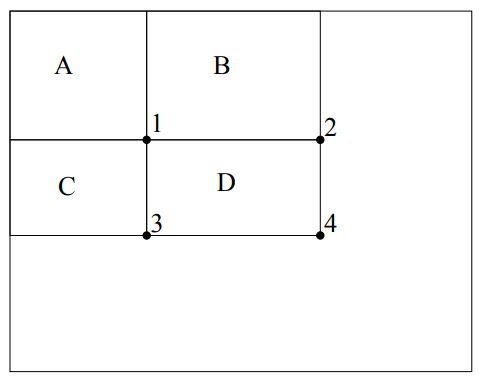
\includegraphics[width=.50\textwidth]{integralImage.png}
  \caption{The sum of the pixels within rectangle  can be
computed with four array references. The value of the integral image at location $1$ is the sum of the pixels in rectangle $A$. The value at location 2 is $A+B$, at location 3 is $A+C$,
and at location 4 is $A+B+C+D$ . The sum within $D$ can
be computed as $4+1-(2+3)$ \cite{Viola01rapidobject}}
  \label{fig:integralImage}
\end{figure}
The second thing that made calculations in the Viola-Jones algorithm so efficient is the use of simple rectangle features.
These features can be calculated very fast on the introduced integral images.
Examples of these rectangle features can be seen in Figure \ref{fig:simpleFeatures}.
\begin{figure}
  \centering
  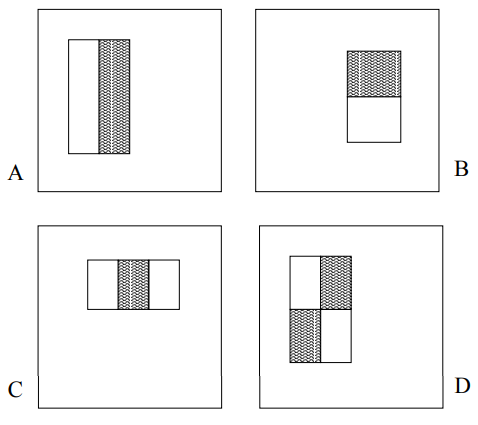
\includegraphics[width=.60\textwidth]{simpleFeatures.png}
  \caption{Example rectangle features shown relative to the
enclosing detection window. The sum of the pixels which
lie within the white rectangles are subtracted from the sum
of pixels in the grey rectangles. Two-rectangle features are
shown in (A) and (B). Figure (C) shows a three-rectangle
feature, and (D) a four-rectangle feature. \cite{Viola01rapidobject}}
  \label{fig:simpleFeatures}
\end{figure}
To learn a small number of important features AdaBoost\cite{FREUND1997119} is used. AdaBoost takes a bunch of weak classifiers and combines their results to a strong classifier.
Another features that was implemented is that the weak classifiers are calculated on subwindows of the original image.
The subwindows refer to a Region Of Interest(ROI).
The classification process works in multiple stages where first the features that have the lowest error rate will be used, while even weaker features come later. 
This so-called \emph{Attentional Cascade} makes it possible to make decisions even in earlier stages which accelerates computation time by a lot.
Although the detection cascade has 38 stages only 10 are used in average.
The Viola-Jones algorithm or variations of it are still used in a wide variety of applications, although classifiers using Convolutional Neural Networks(CNNs)(see Section \ref{ssec:convNets}) have shown to perform better.
Face detection with CNNs are more robust to the alignment of the face in the image. 
While Viola-Jones works very good for frontal faces CNNs can generalize better to also classify non-frontal faces.
Although the CNN approach is more robust it is only possible to run it in realtime on a GPU. This is because neural networks scale very good on GPUs but can be very slow an a CPU for bigger models.
To understand how neural networks work see Section \ref{sec:DeepLearning}.

\subsection{Object tracking}\label{ssec:objectTracking}
%What is it in general
Object tracking is a technique from the field of Image Processing. 
Object tracking became more relevant with the increasing amount of surveillance cameras.
Therefore the research interest in object tracking raised and in the recent years very robust algorithms were developed for object tracking. 
Very important aspects are the online capability as well as scale and translation independence. 
With the MOSSE tracker introduced in 2010 by Bolme et al. in \cite{BolmVisu2010} a robust translation independent approach was presented. In 2014 this approach was enhanced with scale independence by Danelljan et al. in \cite{Danelljan2014}. This approach was implemented in dlib \cite{Dlib} in 2015.
In the following the algorithm will be described.

%Corellation Filters
Correlation based tracking techniques use a filters to model the appearance of the tracking object. These correlation filters indicate how much a parts of an image $f$ correlate with the filter $h$.
The resulting output $g$ is of the same size as $f$ and has peaks in areas, that correlate most with the filter.
In figure \ref{fig:filtersApplied} an example of the application of different filters is given. It is obvious that for the purpose of tracking one of the correlation filters, namely Average of
Synthetic Exact Filters (ASEF)\cite{BolmAver2009}, Unconstrained Minimum
Average Correlation Energy (UMACE)\cite{Savvides2003}, and Minimum
Output Sum of Squared Error (MOSSE)\cite{BolmVisu2010}, suit better than the naive approach since they produce more compact peaks.

\begin{figure}
  \centering
  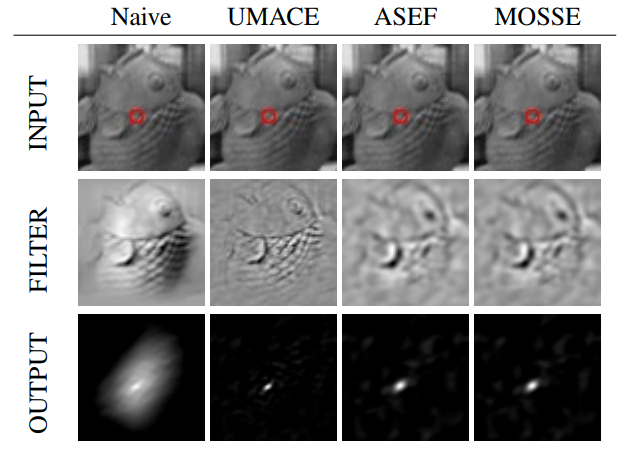
\includegraphics[width=.75\textwidth]{filtersApplied.png}
  \caption{Example of the application of different filters to a sample.  The three correlation
filters produce peaks that are much more compact than the
one produced by the Naive filter. \cite{BolmVisu2010}}
  \label{fig:filtersApplied}
\end{figure}

To track an object the filter $h_0$ is calculated from the first frame $f_0$ given a manually selected position window $p_0$ with the object of interest in center.
In the following frame $f_1$ the filter $h_0$ is applied to a search window. 
The search window is some kind of heuristic assuming the object can only move a limited distance between frames. 
In the resulting output $g_1$, the maximum value corresponds to the position the object moved. 
From this point on the filter $h_n$ is retrained dynamically with the position window $p_n$ of the object in the frame $f_n$.

To reduce computation time the filter is applied in the Fourier domain, since following the Convolution Theorem correlation becomes a element-wise multiplication in the Fourier domain. This results in

\begin{equation}
G = F \odot H^{*}
\end{equation}
where $G$, $F$, $H$ are the output, the input image and the filter in the Fourier domain respectively.
The $\odot$ operator denotes the element-wise multiplication and the $*$ indicates the complex conjugate.
$F = \mathcal{F}(f)$ and $H = \mathcal{F}(h)$ can be calculated with the Fast Fourier Transform (FFT)\cite{Nume2007}
while $g = \mathcal{F}^{-1}(G)$ can be calculated with the inverse FFT. 

While ASEF is averaging over "exact filters" to calculate the resulting filter, MOSSE is calculating the filter by minimizing the Sum of Squared Error (SSE) between the \emph{actual} and \emph{desired} output.
Since the training is conducted in Fourier domain a filter for a given image and output can be calculated element-wise as follows:
\begin{equation}\label{eq:filterSSE}
H^{*}_i = \frac{G_i}{F_i}
\end{equation}
To find a closed form for a filter that fits all given training images SSE is applied to Equation \ref{eq:filterSSE}, resulting in 
\begin{equation}\label{eq:minimize}
\min_{H^*} \sum_{i} |F_i \odot H^* - G_i|^2 
\end{equation}
Bolme et al. derive Equation \ref{eq:minimize} to the closed form 
\begin{equation}\label{eq:MOSSEFilter}
H^* = \frac{\sum_i G_i \odot F^*_i}{\sum_i F_i \odot F^*_i}
\end{equation}
For the initialization of the filter random small affine transformations are applied 
to the tracking window of the first frame. The resulting  perturbations $f_i$ and correspondingly generated outputs $g_i$ are used in Equation \ref{eq:MOSSEFilter} to calculate the initial filter $h_0$. From there on, as mentioned earlier, the online update is applied. Bolme et al. use a running average for the MOSSE filter to update as follows:
\begin{equation}
H^*_i = \frac{A_i}{B_i}
\end{equation}
\begin{equation}
A_i = \eta G_i \odot F^*_i + (1-\eta)A_{i-1}
\end{equation}
\begin{equation}
B_i = \eta F_i \odot F^*_i + (1-\eta)B_{i-1}
\end{equation}
$\eta$ denotes the learning rate, which puts more weight on recent frames and decays the influence of older frames exponentially over time.
%Failure detection
To detect tracking failures or occlusion the Peak to Sidelobe Ratio (PSR) is used. The PSR is a simple measurement of peak strength, which evaluates the peak from the correlation filter in respect to the noise. 
The PSR can be calculated with $\frac{g_{max} - \mu_{sl}}{\sigma_{sl}}$, where $g_{max}$ is the maximum of the correlation output $g$, $\mu_{sl}$ is the mean and $\sigma_{sl}$ is the standard deviation of the sidelobe. 
Whereas the sidelobe is considered to be the output $g$ without an 11 $\times$ 11 pixels area around the peak.
Bolme et al. showed in experiments that UMACE, ASEF and MOSSE filters produce a PSR between 20.0 and 60.0, if tracking is working properly. 
A PSR lower than 7.0 is a strong indicator, that the object is occluded or the tracking failed.
As mentioned earlier the Naive implementation produces peaks not as compact as the other filters, which results in a PSR ranging between 3.0 and 10.0. For the Naive implementation the PSR does not correlate to the tracking quality and therefore no conclusion can be drawn from the PSR.

%Evaluation
Bolme et al. evaluated the MOSSE filter in comparison to the UMACE, ASEF and the naive filter implementation on seven commonly used and freely available test videos from \url{http://www.cs.toronto.edu/\textasciitilde dross/ivt/}.
The results presented in Figure \ref{fig:eval} show that the MOSSE filter outperforms the other approaches in nearly every situation. %\cite{BolmVisu2010} 

\begin{figure}
\centering
  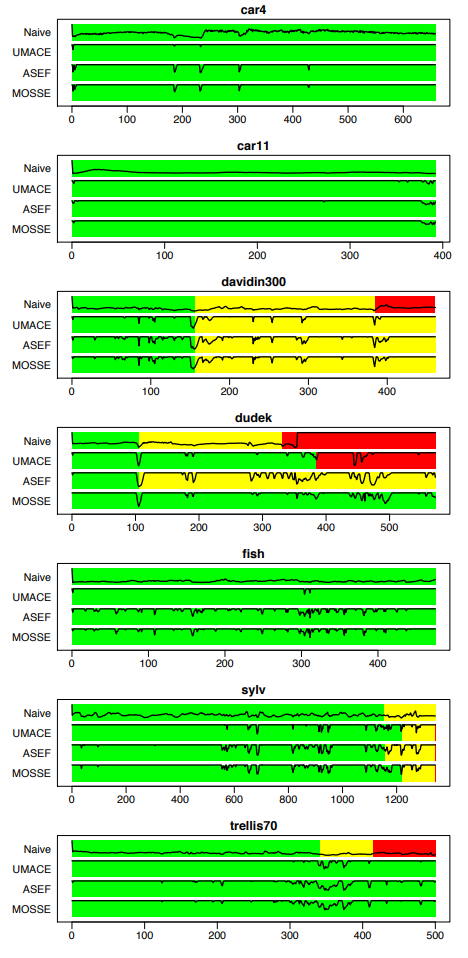
\includegraphics[width=.75\textwidth]{eval.png}
  \caption{This figure shows the performance of the filter based
trackers on all seven of the video sequences. Each output video
was hand annotated where Green indicates a good track, Yellow
indicates the track drifted off center, and Red indicates tracking
failure. The black lines shows PSR that was clipped to the range
[0,20] and indicates the quality of the track for each frame of the
video. \cite{BolmVisu2010}}
  \label{fig:eval}
\end{figure}

%Scale independency from Danelljan et al.
As mentioned earlier the MOSSE filter approach is extended by Danelljan et al. in \cite{Danelljan2014} with a scale estimation to increase robustness in situations where large scale variations appear.Therefore a separate scale correlation filter is used.
This filter is updated with a training example $f$, which is constructed from features, that use different patch sizes centered around the target.
This filter is applied to the target location calculated by the translation filter.
This technique saves some computation time and is possible because the difference in scale between to successive frames is normally smaller than the difference in translation. This enables the approach to accurately and computationally efficient estimate translation and scale of a tracking object in a video sequence.




% Learning algorithms
\section{Learning Algorithms}\label{sec:learningAlgorithms}
This section describes all the theoretical parts of a Learning Algorithm. Starting from the data and how to handle it going to different approaches to make sense out of data ending in specific learning algorithms.
\subsection{Data}\label{ssec:dataTheory}
Data Scientist are coming up with new algorithms to solve specific problems nearly everyday and they lead to astonishing results in the field of Natural Language Processing and Image Classification.
New Algorithms and better Hardware brought fields like Optical Character Recognition, Automatic Speech Recognition and Image Classification to a near-human level. 
With this new achievements and a growing basis of publicly available datasets people tend to forget that the foundation of learning is the data. Exactly these huge publicly available datasets, like ImageNet\cite{ImageNet} with more than 14 million images in over 20 thousand categories, are the reason why Data Scientist could develop new algorithms and effectively use Deep Learning.


The fanciest algorithms with cutting edge hardware will not learn the desired relation if the data is corrupted or simply not suited for the task.
So when it comes to developing a learning algorithm it is important to know what the goal is and what relation the data can provide.
For a lot of projects publicly available datasets offer a good starting point to either use the data directly or extract a new dataset for a specif task from it. 
\url{https://www.kaggle.com/datasets} offers a wide range of datasets for all kinds of applications.

After carefully selecting the data it is important to split the data in three different parts. 
Most of the publicly available datasets are already divided in \emph{training data}, \emph{validation data} and \emph{test data} and newly constructed datasets should be divided in the same categories.
With these three subsets it is possible to effectively evaluate an algorithm.
This brings the advantage of comparability for different algorithms on the same problem.
The subsets have the following functions:

\begin{description}
\item[Training Data]\hfill \\
The training data is the biggest subset of the dataset and takes normally around 70-80\% of the data. This data is used to train the learning algorithm.
\item[Validation Data]\hfill \\ 
The validation data is used to validate the the algorithm while searching for suitable hyper parameters(see \ref{ssec:hyperP}) and prevent overfitting(see section \ref{ssec:overfitting}).
The validation data normally takes around 10-15\% of the data.
\item[Test Data]\hfill \\ 
The test data is only used once in the very end to evaluate the algorithm.
The test data normally takes around 10-15\% of the data.
\end{description}

\begin{figure}
\centering
  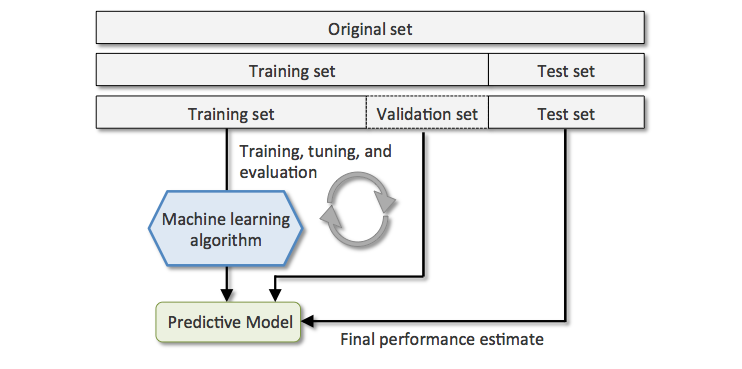
\includegraphics[width=.75\textwidth]{training_validation_test.png}
  \caption{Dividing and using a dataset correctly \cite{DataSplit}}
  \label{fig:dataSplit}
\end{figure}


One could ask if the test data evaluates the algorithm what is the validation data for?
While searching for a good model for the problem the hyper parameters will be adjusted to get the best results on the validation data. 
The process of searching for the perfect hyper parameters can be viewed as \emph{learning} only that it is not the algorithm that learns the best parameters to satisfy the training data, but the Data Scientist that learns the best hyper parameters to satisfy the validation data. This process is as well prune to overfitting.
This also explains why the test data can only be used once.
Changing anything about the model because of the performance of the test data, the assessment of generalizability will be flawed.

In terms of constructing a dataset three aspects should be considered very carefully.

\begin{description}
\item[Representativeness of the data]\hfill \\
It is important that training, validation and test data represent the whole dataset. 
In a classification task with 10 classes, where the training data holds only samples from the first 8 classes, while validation data only holds class 9 and the test data only holds samples of class 10, the algorithm can obviously never perform well on the validation or test data. 
To prevent such behavior the dataset should be randomly shuffled.
\item[Redundancy of the data]\hfill \\ 
Redundant data happens a lot, that is basically no problem. 
The problem comes up, when the sample ends up in training data and validation or test data.
When that happens evaluation(validation or test) is actually happening on some part of the training data, which flaw the assessment of generalizability.
\item[Time dependency of the data]\hfill \\ 
If the task is to predict the future from the past it is important not to shuffle the dataset randomly, because otherwise the model will be trained on future data and evaluated on past data which is the opposite of what was the goal.
\end{description}

\subsection{Preprocessing}\label{ssec:preprocessing}
After choosing the right data for the desired task and dividing it into training, validation and test data often another step is necessary before the training can start.
This step is called preprocessing and describes the transformation of the data into a shape, that fits the selected algorithm best.
These transformations can be arbitrary but the following transformations are common:
\subsubsection{Data Cleaning}
Data cleaning deals with the detection and correction(or removal) of duplicates, corrupted samples and outliers. 
If corrupted samples get into the learning process, it can influence the results a lot. For example if a feature is out of its known range, it can be rejected or corrected before even considered in the training process.
\subsubsection{Normalization}\label{ssec:normalization}
A lot of the learning algorithms have problems if features have a great difference in scale between each other. 
With this in mind it makes sense to normalize the features to a common range. 
It is common practice to normalize the features to a mean of 0 and a standard deviation of 1. Some algorithms are expecting values in this shape or at least working optimal with those. If gradient descent is used to optimize the model parameters this helps to keep the gradient of the loss function at small values.\cite{CholDeep2018}

\subsubsection{Feature Extraction}\label{ssec:featureExtracion}
A dataset consists of samples which describe a observation.
These samples consist of features and labels (if we consider supervised learning). Features are normally denoted as 
$\mathbf{x} = \left\langle x_{0}, x_{1}, \cdots , x_{n-1}, x_{n} \right\rangle$ while labels are denoted as $\mathbf{y} = \left\langle y_{0}, y_{1}, \cdots , y_{m-1}, y_{m} \right\rangle$
Since the general goal of learning algorithms is to find a mapping between $\mathbf{x}$ and $\mathbf{y}$ it makes sense to take a closer look to the features.
Features can be of very different shape, but the more compact the information is represented the easier is it for the learning algorithm to find a mapping.
In Figure \ref{fig:featureClock} an example of the same information in different shapes is given.  
\begin{figure}
\centering
  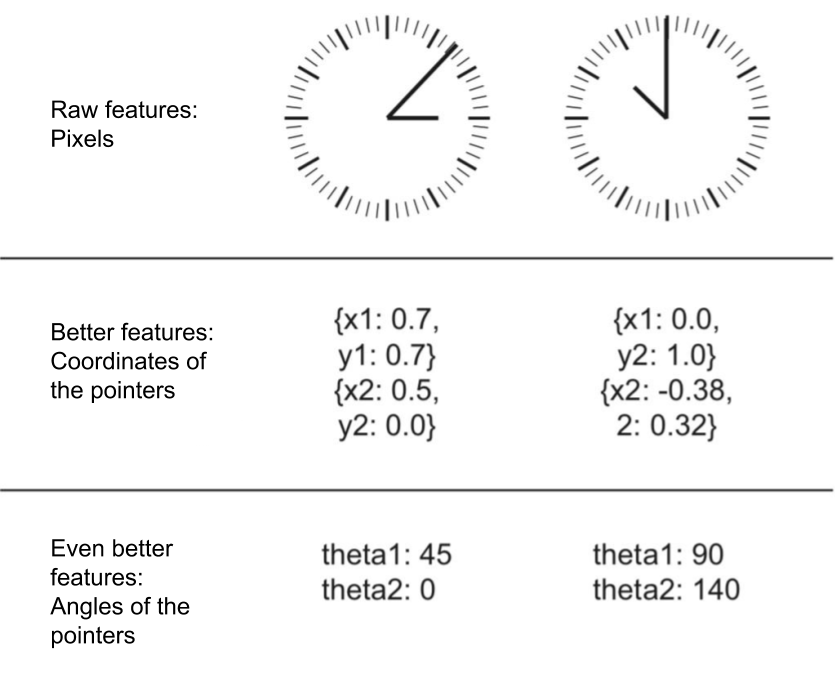
\includegraphics[width=.75\textwidth]{featureClock.png}
  \caption{Different types of features for the same problem \cite{CholDeep2018}}
  \label{fig:featureClock}
\end{figure}
This example shows very nice how feature extraction can decrease the input shape and size by a lot, which makes learning essentially easier. 
Assuming the image of the clock is $64 \times 64$ pixels the input would be a two-dimensional array with 4096 values.
Learn a mapping between this input values and the time as output value is a relatively complex task that would need a CNN to be trained. 
So using the raw features would lead to a significant computational effort.
In contrast extracting the coordinates of the tip of the pointer would end up in an 1-dimensional input shape with four values. 
Learning the mapping between the coordinates and the time is essentially easier.
Taking it even further changing the coordinate system from a Cartesian coordinate system to a polar coordinate system the input can be reduced to two values.
And for that learning wouldn't be necessary. Rounding of the values and putting the corresponding time in a dictionary would be enough.

Domain knowledge can be very helpful to make learning easier for the algorithm.
Before Deep Learning became really applicable feature extraction was a big and important part in data science.
Good features decided about the quality of shallow learning approaches.
In Deep Learning the hypothesis space is essentially bigger which makes it possible to learn those features on the fly.
For learning these features a lot of data is needed, so if only little data is available feature extraction is still important.
It is important to have in mind, that the features in Deep Learning are learned automatically, so it makes sense to verify the learned features. 

For example if a CNN should classify if a male or female is in a picture and the dataset consists of images from males and females, but females are always captured in front of a white background and males are always captured in front of a black background the CNN will most certainly learn that and will perform poorly on images with blue background.
Humans wouldn't take the background in consideration because they already know the domain of the problem.
The CNN doesn't know anything, so everything will be considered.

\subsection{Categories of Learning}
In general learning can be viewed as finding a mapping from an input $\mathbf{x}$ and an output $\mathbf{y}$.
Figure \ref{fig:learning} shows a schematic overview on how to come from data to a hypothesis that can make predictions after training.

\begin{figure}
\centering
  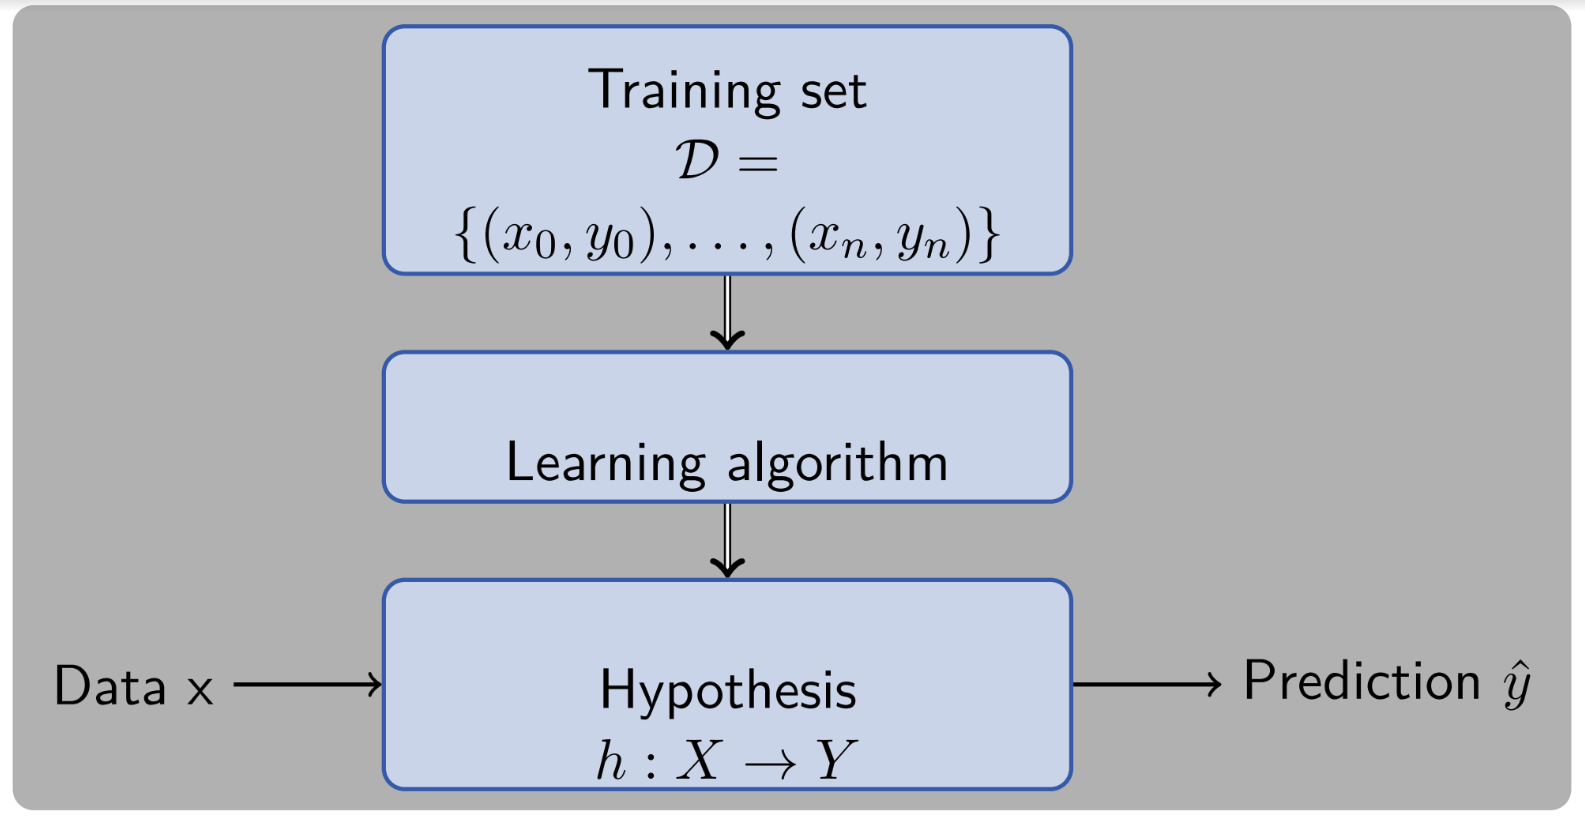
\includegraphics[width=.75\textwidth]{learning.png}
  \caption{The overall structure of learning.\cite{LVDFKI}}
  \label{fig:learning}
\end{figure}

Learning can be divided into four different categories.
At some point they can overlap a little but most of the time problems can be classified in one of the following categories.

\subsubsection{Supervised Learning}
In Supervised Learning the learning algorithm is fed with labeled data and the goal is to learn a hypothesis $h$ that maps the input $\mathbf{x}$ to the output $\mathbf{y}$.
As shown in Figure \ref{fig:learning} the Training set $\mathcal{D}$ consists of input values $x_i$ and their corresponding output value $y_i$. These labels are often also called the \emph{ground truth} because this is the information, that is true and should be learned.
This is given to a learning algorithm, which calculates a hypothesis(this is often also called a model) of the data, which is able to predict an output $\hat{y}$ for a given input $x$.

There are basically two types of Supervised Learning.
If the output data is in the discrete domain the task is called \emph{Classification}.
A very easy example would be the classification of handwritten digits, where the input would be a grid of pixels(an image) and the output would be an integer from 0 to 9. 
(Example from the MNIST dataset for handwritten digits\cite{YannGrad1998} available under \url{http://yann.lecun.com/exdb/mnist/}) 

In contrast if the output data is in the continuous domain the task is called \emph{Regression}.
An easy example for regression would be to predict the price of a house by attributes like \texttt{per capita crime rate by town}, \texttt{Average number of rooms per dwelling}, \texttt{Index of accessibility to radial highways} and many more. 
(Example from the Boston Housing dataset\cite{Harrison78} available under \url{https://www.kaggle.com/c/boston-housing}) 

Supervised Learning is by far the category with the most applications.
This is because it is relatively easy to evaluate the accuracy of the developed learning algorithm, because the ground truth is available to apply several metrics(see section \ref{ssec:lossFunc}) to the results.

\subsubsection{Unsupervised Learning}
Unsupervised Learning describes a category of learning where the ground truth is not known. 
For Unsupervised Learning the Training Data $\mathcal{D}$ shown in figure \ref{fig:learning} would lack the labels $y_0$ to $y_n$.
With no ground truth available the learning algorithm can only find previously unknown patterns in the data.

\emph{Clustering aims at partitioning $n$ observations into $k$ clusters.
Observations that are assigned to the same cluster should be more
“similar” than those belonging to different clusters.}\cite{LVDFKI}

Clustering helps Data Scientist to to understand the data better and to discover existing correlations in it.
Sometimes clustering is an important first step towards a Supervised Learning task. 
As stated before Unsupervised Learning is harder to evaluate because there is no ground truth to evaluate the results on.
Figure \ref{fig:clustering} shows some examples of clustering algorithms and how they perform in different scenarios.

\begin{figure}
\centering
  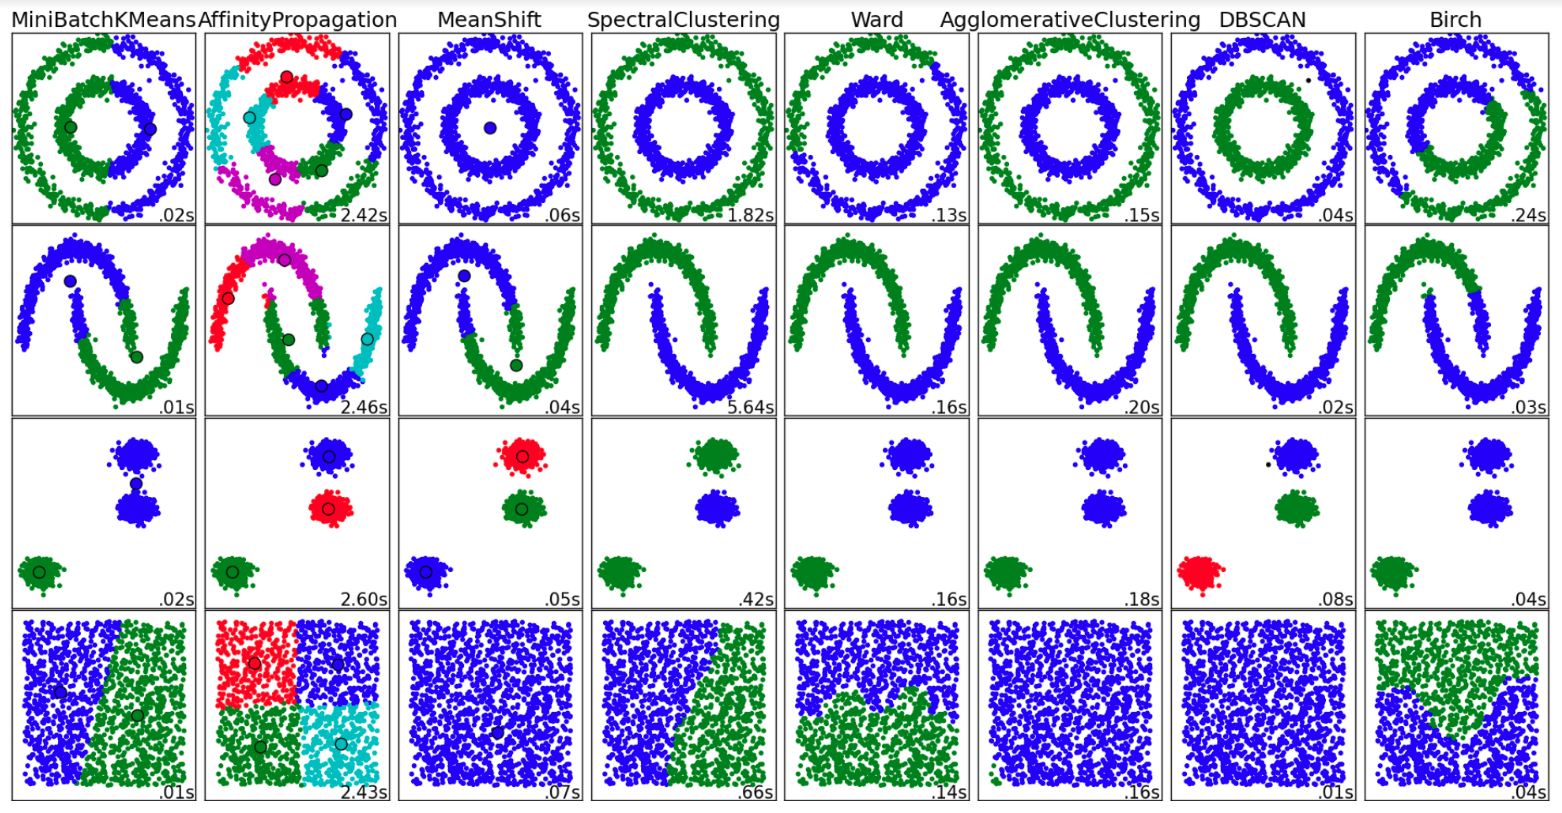
\includegraphics[width=.75\textwidth]{clustering.png}
  \caption{clustering algorithms and how they perform in different scenarios.\cite{LVDFKI}}
  \label{fig:clustering}
\end{figure}

\emph{Dimension Reduction} is another technique that can be performed unsupervised.
The goal of Dimension Reduction is to reduce the dimensionality of the input data.
An example of Dimension Reduction would be the Principal Component Analysis, which finds the features with the highest variation in the data. The highest variation is closely related to the meaningfulness of the features. 
If specific features have no or nearly no meaningfulness they can be dropped and therefore reduce the dimensionality of the data.



\subsubsection{Self-supervised Learning}
Self-supervised Learning is more or less a sub category of Supervised Learning, where labels are automatically extracted from unlabeled data, to then start a supervised learning process. 
A simple example for Self-supervised Learning would be to predict the next frame of a video sequence or the next word of a sequence of words.
Here no labels are available but sequences have the neat ability, that they have implicit output values when it comes to predicting the next element of a sequence.
For the example with sequences of words it is possible to just have a bunch of phrases and extract labeled sequences by always taking $x$ words as input and the $x+1$ word as the label.


\subsubsection{Reinforcement Learning}
Another very interesting category of learning is \emph{Reinforcement Learning}, where an \emph{Agent} learns to conduct different \emph{Actions} in an \emph{Environment} to maximize a \emph{Reward}.
An Example would be a learning Agent that takes the screen of a video game as the input and learns to perform the best actions to gain the most points.
This category gained a lot of attention lately through the astonishing performance of AlphaGo \cite{AlphaGo} to be the first AI, that won against a human champion.


\section{Deep Learning}\label{sec:DeepLearning}
As described in Section \ref{sec:approach} the VVAD is implemented using a LSTM-FCN, which is a neural network containing a convolutional part to model the spatial features and a recurrent part to model the temporal features. 
In this section, all theoretical aspects of an LSTM-FCN are explained.
\subsection{Artificial Neural Network(ANN)}
An Artificial Neural Network can be described as the attempt to model the human brain in a computer. As the human brain is very complex and research in this field is not certain about every aspect and a large part is still completely unexplored, the connection between an ANN and the human brain is very loose and only models the parts, that scientists are very certain about. 
This is the fact that the brain consists out of around 100 billion of neurons interconnected in a complex network structure \cite{Herculano09}.
The "wire" that connects neurons is called axon and is in fact acting like a wire that transmits  small potentials  between the neurons.
The axons can have different conductivity depending on how frequently they are used.
This is very important because it is one of the ingredients how human can learn. 
This concept is called \emph{weights} in an ANN. How \emph{weights} are implemented in an ANN and how that impacts learning will be discussed later.
One neuron can have multiple incoming and one outgoing axons. 
Without mentioning all the biochemical processes happening at this point, one can simplify and say all incoming axons merge into the axon hillock where, if a certain threshold is reached the neuron invokes a potential itself ("fires").
The merging of axons is a summation of the transported potential, where the potential can be excitatory (having a positive influence on the sum) or inhibitory (having a negative influence on the sum). In an ANN excitatory potentials would be positive \emph{weights} while inhibitory potentials would be negative \emph{weights}.
\cite{BGDFKI}
So one neuron can be seen as some kind of a gate which decides if the sum of some incoming signals is worth to fire an outgoing signal.
And the whole network of neurons can be seen as sieve that allows only specific paths for the potentials to go through the network. 
The well known experiment called \emph{Pavlov's Dog} is a good example to show how these paths work.

\paragraph{Pavlov's Dog:}
A Dog is presented two different stimuli. As presented in Figure \ref{fig:pavlov} these are a unconditioned stimulus(food) and a neutral stimulus(bell ringing). The unconditioned stimulus produces a unconditioned response, which is salivation in the case of Pavlov's dog. The goal in the experiment is to show that it is possible to condition the dog to show the same response on the bell ringing.

\begin{figure}
\centering
  \includegraphics[width=.75\textwidth]{Classical_Conditioning_Diagram.png}
  \caption{Classical Conditioning Diagram \cite{pavlovsDog}}
  \label{fig:pavlov}
\end{figure}

\paragraph{} %pseudo end of the paragraph before
To understand how the dog \emph{learns} to salivate on the ringing of the bell the analogy of the paths is used.
The smell of the food activates some nerve cells in the dog's nose. The invoked potentials are forwarded to the brain, where the \emph{sieve} decides which action is mapped to the incoming signal. The signal takes a path over several neurons to end up in a place which activates the salivation. 
This path was already there and is probably one of the \emph{preprogrammed} paths a dog was born with. 
These \emph{preprogrammed} paths are learned evolutionary.
If the dog is presented the neutral stimulus salivation will not be activated because there is no path between the nerve cells from the ears and the neurons that activate the salivation.
As the dog is presented both stimuli the brain gets the described two inputs.
Another very important mechanism for learning takes effect here.
If something "good" is happening all recently active axons will be strengthened which results in a higher conductivity.
If something "bad" is happening the effect is flipped.
ANNs try to reproduce this mechanism mathematically by a procedure called backpropagation(see section \ref{ssec:backProp}).
The brain has very complex mechanisms to decide what is "good" and "bad". This is not relevant for the example and will not be discussed any further. 
In the example the assumption holds that food is something "good" and therefore all recently active axons will be strengthened. 
This means that also all the axons corresponding to the bell ringing will be strengthened. 
If the axons' conductivity is higher a higher potential can be transmitted and therefore reach a higher summed potential in other neurons. If the potential is higher than a certain threshold this neuron will fire. 
This means the path from the neurons corresponding to the bell ringing will enlarge every time both stimuli are presented at the same time.
After a while this will eventually lead to the development of a path between the bell ringing and the salivation neurons.
This explains, why the dog \emph{learned} to salivate on bell ringing.
Knowing this it makes also sense that the effect will vanish if the bell ringing is presented too often without the reward of the food, because being tricked is considered as something "bad" by the brain.
In the human brain neurons can be connected very arbitrary, while modern ANNs normally structure their artificial neurons in so called \emph{Layers}.
Figure \ref{fig:3layers} shows a ANN with three layers.
Each layer consists of a number of artificial neurons that are connected to the previous and subsequent layer.

\begin{figure}
\centering
  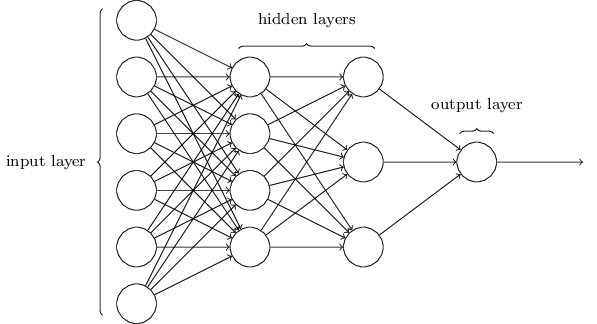
\includegraphics[width=.75\textwidth]{3layers.png}
  \caption{A neural network with one input layer, two hidden layers and an output layer.\cite{Nielsen2015}}
  \label{fig:3layers}
\end{figure}

\subsection{Artificial Neuron}\label{artificialNeuron}
The smallest element of an ANN is the artificial neuron.
The modern artificial neurons are inspired by the concept of a perceptron, which was developed by Frank Rosenblatt in the 1960s \cite{rosenblatt1962principles}.
The perceptron is the first approach to model a neuron in a computer.
A perceptron can have multiple inputs and one output, just like a neuron in the human brain.
Figure \ref{fig:perceptron} shows an example of a perceptron with the three inputs $x_1, x_2, x_3$.

\begin{figure}
\centering
  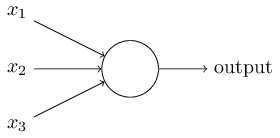
\includegraphics[width=.75\textwidth]{perceptron.png}
  \caption{A perceptron with input $x_1, x_2, x_3$ \cite{Nielsen2015}}
  \label{fig:perceptron}
\end{figure}

To calculate the output Rosenblatt introduced the concept of \emph{weights}, which describe how important a specific input is for the output.
The classical perceptron produces a binary output, which is calculated using equation \ref{eq:perceptron}.
\begin{equation}\label{eq:perceptron}
output = \left\{\begin{matrix}
0 & \mathrm{if} \sum _j w_j  x_j\leq \mathrm{threshold}\\ 
1 & \mathrm{if} \sum _j w_j  x_j>  \mathrm{threshold}
\end{matrix}\right.
\end{equation}
This equation is the \emph{activation function} of the perceptron. 
It basically decides whether the perceptron fires or not.
If equation \ref{eq:perceptron} is applied with the dot product of the vector $w = \left\langle w_1, w_2, ..., w_n  \right\rangle$ for the weights and $x = \left\langle x_1, x_2, ..., x_n  \right\rangle$ for the inputs, it is possible to move the threshold to the other side of the inequality. Furthermore the threshold is replaced by an new variable called \emph{bias} in the following fashion: $b \equiv -\mathrm{threshold}$

This leads to equation \ref{eq:heaviside} which is basically the Heaviside step function

\begin{equation}\label{eq:heaviside}
output = \left\{\begin{matrix}
0 & \mathrm{if} \ w \cdot x + b\leq 0\\ 
1 & \mathrm{if} \ w \cdot x + b >  0
\end{matrix}\right.
\end{equation}

Rosenblatt proved that a single perceptron can implement the logic operation \texttt{NAND} which is a basic logic operation. 
This means all other logic operations can be build using a \texttt{NAND}. 
This is shown in the following example:

Figure \ref{fig:NAND} shows a perceptron with two inputs and the corresponding \emph{weights} of $-2$ and a \emph{bias} of 3.
\begin{figure}
\centering
  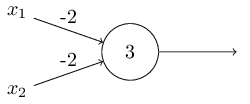
\includegraphics[width=.75\textwidth]{NAND.png}
  \caption{The perceptron implements a logic \texttt{NAND} gate \cite{Nielsen2015}}
  \label{fig:NAND}
\end{figure}
Giving the input $x_1=0;x_2=0$ the perceptron will output $1$, hence $(-2) \cdot 0 + (-2) \cdot 0 + 3 = 3$ is positive. 
Doing the same calculation for the input where either one of the inputs is $0$ and the other is $1$ shows the same output but if both input values are $1$ the formula produces an output of $0$, since $(-2) \cdot 1 + (-2) \cdot 1 + 3 = -1$ is negative.
With the \texttt{NAND} gate it is for example possible to build the bitwise addition.
Figure \ref{fig:NANDADD} shows how multiple perceptrons can be linked to a network to implement the addition of two input bits with a carry bit which depicts if both inputs are $1$ which would lead to a resulting sum of $2$.
$2$ is not mappable in a single bit representation, therefore the carry bit shows the overflow.

\begin{figure}
\centering
  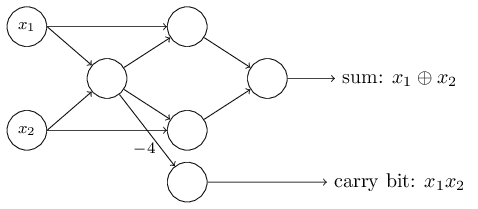
\includegraphics[width=.75\textwidth]{NANDADD.png}
  \caption{A network of perceptrons building the bitwise addition of two inputs. All weights are -2 and all biases are 3 as shown in Figure \ref{fig:NAND}. The -4 means that the input is the same for $x_1$ and $x_2$ of that perceptron \cite{Nielsen2015}}
  \label{fig:NANDADD}
\end{figure}

This already shows that networks of perceptrons are quite powerful but the problem is, that in the given example all weights were given and the goal of \emph{Learning} is to abstract these out of given samples.
There are two main problems when it comes to learning the weights of a classical perceptron.
\begin{itemize}
\item[1.] The state of the art way to train neural networks is by using gradient descent (see Section \ref{ssec:gradientDescent}) with backpropagation (see Section \ref{ssec:backProp}).
Backpropagation requires the activation functions of the artificial neurons to be differentiable. 
Hence the Heaviside step function used by the classical perceptron is not differentiable at $x = 0$ and has a gradient of $0$ anywhere else, the gradient descent method won't work here.
\item[2.] Mathematically speaking, \emph{learning} the weights for a neural network is an optimization problem. 
The goal here is to find the weights that produce the smallest error on the output.
Optimizing in this case is only possible if small changes in the weights cause only small changes in the resulting error.
Since the Heaviside step function can only produce $0$ and $1$ as output, it does not fulfill this requirement.
\end{itemize}

\subsection{Activation Function}
As described earlier the \emph{activation function} is a function that decides whether an artificial neuron fires or not. 
Since the classical perceptron does not fulfill the requirements to be used with backpropagation and gradient descent new activation functions needed to be developed to make neural networks a solvable optimization problem.
Additionally to the requirements that the activation function needs to be differentiable and small changes in the weights should have a small impact on the output, non-linearity is a very important requirement.
A combination of layers of artificial neurons with linear activation functions can only lead to a overall linear function to model the data.
To model non-linearity in data it is important to have non-linear activation functions.
Following three of the most used and well known activation functions will be presented.
\paragraph{Sigmoid Function:}
The sigmoid function, sometimes also known as the logistic function, gives an output between $0$ and $1$. 
It is defined by by equation \ref{eq:sigmoid} and Figure \ref{fig:sigmoid} shows the course of the resulting curve.
\begin{equation}\label{eq:sigmoid}
sigmoid(x) = \frac{1}{1 + e^{-x}}
\end{equation}
\begin{figure}
\centering
  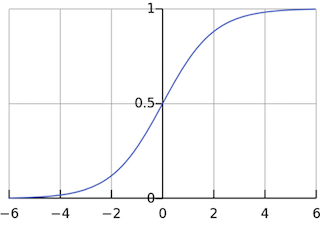
\includegraphics[width=.50\textwidth]{sigmoid.png}
  \caption{The shape of the sigmoid function \cite{Chris2017}}
  \label{fig:sigmoid}
\end{figure}
The sigmoid function fulfills all the requirements to be used with gradient descent and backpropagation. 
It is differentiable as there are no hard edges in the curve and it shows small and steady changes for small changes in the input and it is obviously non-linear. Despite all these positive aspects it has one major drawback.
The sigmoid function is at risk of facing the problem of the \emph{vanishing gradient}. The vanishing gradient will be discussed in a little more depth in Section \ref{ssec:backProp}, but the problem is very visible for very large positive or negative input values.
The output values for these input values are very close to either $0$ or $1$ but don't change a lot in this areas. 
This means the gradient is very small or even vanishes and this means gradient descent can no longer work to find the minimal error, which means there is no \emph{learning}.
This effect gets even stronger the more layers are stacked upon each other and can make the training of deep models very slow to impossible.

\paragraph{Tanh Function:}
The tanh function is very similar to the sigmoid function.
It is defined by Equation \ref{eq:tanh} and Figure \ref{fig:tanh} shows the course of the resulting curve.
\begin{equation}\label{eq:tanh}
tanh(x) = \frac{e^x - e^{-x}}{e^x + e^{-x}}
\end{equation}
\begin{figure}
\centering
  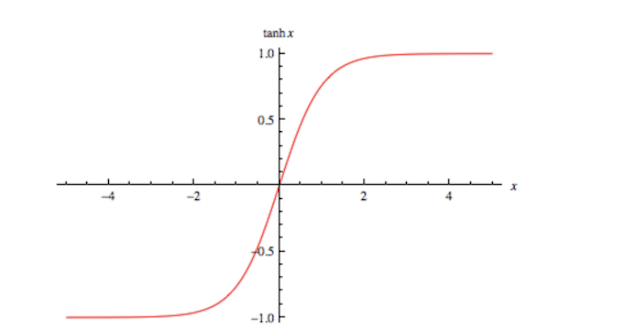
\includegraphics[width=.60\textwidth]{tanh.png}
  \caption{The shape of the tanh function \cite{Chris2017}}
  \label{fig:tanh}
\end{figure}
Figure \ref{fig:tanh} shows that sigmoid and tanh functions are very similar except that the tanh function maps the output to values between $-1$ and $1$.
Because of the close similarity the tanh function shares the same drawbacks as the sigmoid function.

\paragraph{ReLu (Rectified Linear Unit):}
The ReLu activation function is quite different to the sigmoid and tanh function. It is defined by Equation \ref{eq:relu} and Figure \ref{fig:relu} shows the course of the resulting curve.
\begin{equation}\label{eq:relu}
relu(x) = max(0, x)
\end{equation}
\begin{figure}
\centering
  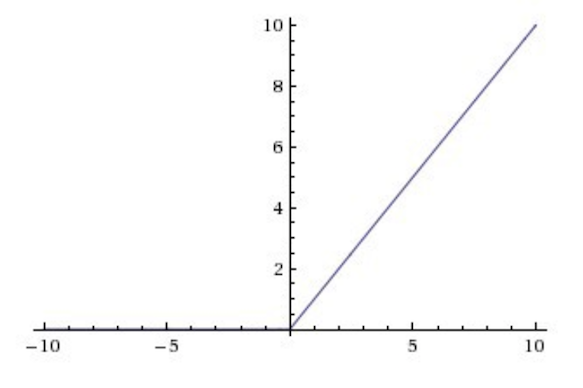
\includegraphics[width=.60\textwidth]{relu.png}
  \caption{The shape of the ReLu function \cite{Chris2017}}
  \label{fig:relu}
\end{figure}
On the first sight the ReLu looks very linear and intuitively one wouldn't expect it to perform very well.
As ReLu is computational very efficient and it is known to have no vanishing gradients Johnson et al. proposed to use the ReLu as the default non-linearity \cite{ConvNNs}.
Although the ReLu can handle the problem of \emph{vanishing gradients} it develops a new problem.
The \emph{dying ReLu} describes a phenomenon where a single artificial neuron will never be able to fire and therefore can be described as dead.
This happens when the activation value generated by an artificial neuron is $0$ during the forward pass over some iterations which causes it's weights to go to $0$ and it will never be able to fire again.

\subsection{Gradient Descent}\label{ssec:gradientDescent}
As mentioned earlier \emph{Learning} is basically an optimization process with the goal to find the parameters $\theta$ that minimize a loss(sometimes also referred to as cost) function $L(\theta)$(loss functions are explained in more depth in Section \ref{ssec:lossFunc}).
The gradient of the loss function is defined in equation \ref{eq:gradient} and \ref{eq:gradient_i}
\begin{equation} \label{eq:gradient}
g = \nabla_{\theta} L(\theta)
\end{equation}
\begin{equation} \label{eq:gradient_i}
g_i = \frac{\partial}{\partial\theta_{i}}  L(\theta)
\end{equation}
The gradient is basically the change in a function. 
Considering a linear regression model defined as 
\begin{equation}
y = \beta_0 + \beta_1 x_1
\end{equation}
the best values for $\beta_0$ and $\beta_1$ can be found using some x-y-points that should model the line (see Figure \ref{fig:points}), a loss function(in this case the mean squared error(MSE) is a good fit) and gradient descent as optimizer.
\begin{figure}
\centering
  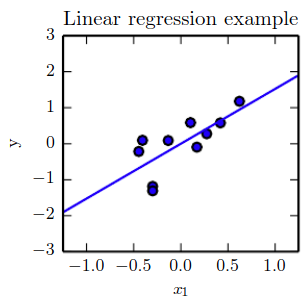
\includegraphics[width=.50\textwidth]{points.png}
  \caption{A linear regression problem, with a training set consisting of ten data points \cite{Goodfellow-et-al-2016}
}\label{fig:points}
\end{figure}
MSE will be discussed in detail in Section \ref{ssec:lossFunc} for now it is only important to know, that MSE maps the loss for the parameters $\beta_0$ and $\beta_1$ and the goal is to find its minimum.
Figure \ref{fig:gradientDescent} shows how the loss behaves plotted over $\beta_0$ and $\beta_1$.

\begin{figure}
\centering
  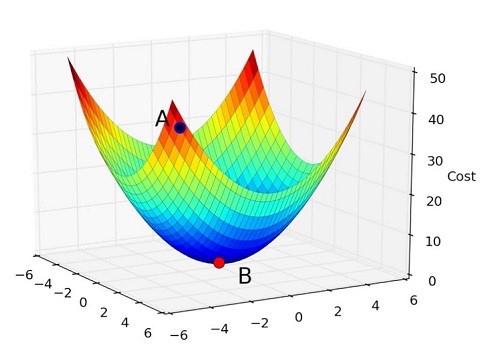
\includegraphics[width=.60\textwidth]{gradientDescent.jpeg}
  \caption{The goal for gradient descent is to go from a randomly initialized point A to the minimum in point B \cite{gradDescent}
}\label{fig:gradientDescent}
\end{figure}
The gradient descent is a iterative method, which only considers the gradient of a function and depending on the value of the gradient it will move the parameters towards the minimum.
Mathematically this can be formulated as 
\begin{equation}\label{eq:gradDescUpdate}
\theta_{n+1} = \theta_n - \alpha \nabla L(\hat{y}, y)
\end{equation}
$\hat{y} = y_{\theta_n}(\mathbf{x})$ is the prediction made from the model with the parameters $\theta_n$ \cite{ValdenegroToro2019DeepNN}.
The update for the parameters from equation \ref{eq:gradDescUpdate} can be computed for a predefined number of steps or until the change in the loss or the gradient stays under a predefined value for a predefined number of iterations.
$\alpha$ in equation \ref{eq:gradDescUpdate} is the \emph{Learning Rate}, which decides how much influence one update step has on the parameters.
In the given example of a linear regression model the parameters 
$\beta_0$ and $\beta_1$ would be optimized coming from point A and ending up in the minimum in point B.
Equation \ref{eq:gradDescUpdate} can be applied in the same way to deep neural networks. As the number of parameters for these deep neural networks (DNNs) is essentially bigger, the loss surface can not be plotted in a human-readable way. 
With a higher dimensionality of the parameters the hypotheses space will grow exponentially. This phenomena is known as the \emph{curse of dimensionality} which also explains why Deep Learning needs so much data to efficiently learn.
%influence of LearningRate and lossSurface
The success of gradient descent largely relies on the following two factors:
\paragraph{Learning Rate}
As mentioned earlier the \emph{Learning Rate} decides how much influence one update step has on the parameters. 
It is very important to set a good value here. If the Learning Rate is to big the optimization process can get very unstable and the minimum will not be reached due to overshooting. 
On the opposite if the Learning Rate is to small convergence can take too long as depicted in Figure \ref{fig:lr}.
\begin{figure}
\centering
  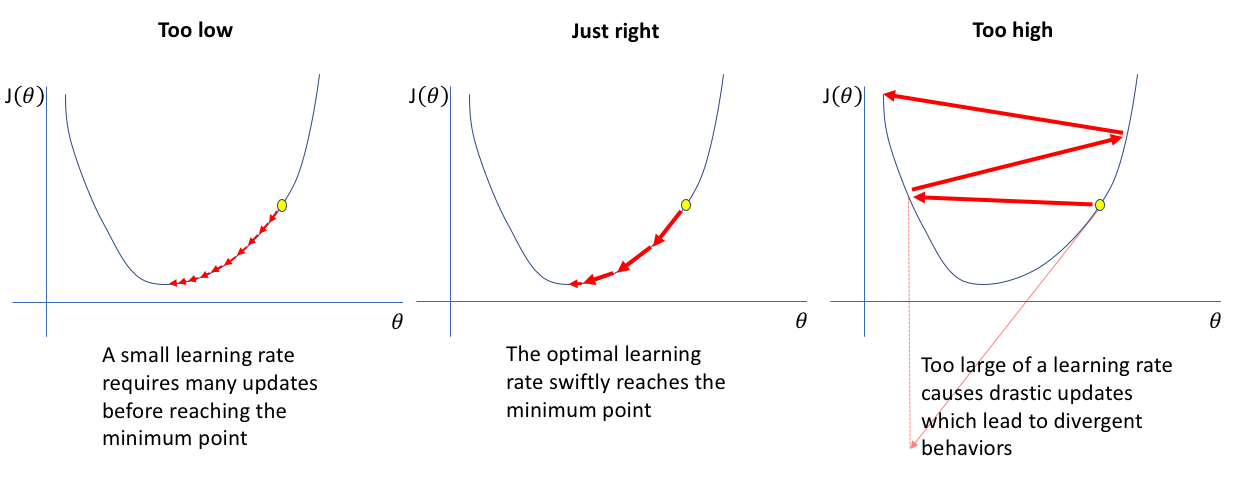
\includegraphics[width=\textwidth]{lr.png}
  \caption{Setting the correct learning rate is essential for good and fast convergence \cite{lr}
}\label{fig:lr}
\end{figure}
Typical values of the learning rate are $\alpha \in [0,1]$, and common starting values are $10^{-1}$ or  $10^{-2}$.\cite{ValdenegroToro2019DeepNN}. 
It is even common practice to change the Learning Rate during training. 
Common approaches are to
decrease the learning rate by a factor after a certain number of
iterations, or to decay the learning rate by a factor after each step. \cite{ValdenegroToro2019DeepNN}
\paragraph{Loss Surface}
Figure \ref{fig:gradientDescent} shows a very simple Loss Surface, for which it is imaginable easy to find the minimum but models more complex than the linear regression produce more complex loss surfaces. 
If the gradient in the loss surface gets to small or to big gradient descent is prone to the problem of vanishing / exploding gradient, because backpropagation in DNNs makes these values become more extreme.
The optimal loss surface is convex and has a smooth geometry.
In practice a non-convex loss function
is not a big problem, and many theoretical results show that the
local optima in deep neural networks are very similar and close
in terms of loss value. \cite{ValdenegroToro2019DeepNN}
\paragraph{} %pseudo end of the paragraph before
Gradient Descent comes in different variations.
The update rule given in equation \ref{eq:gradDescUpdate} is actually called Batch Gradient Descent and takes all training samples into account at once. 
This method basically takes the whole "batch" of training samples to do the update. 
This implicitly assumes that the whole dataset fits into memory. 
Recalling the curse of dimensionality this can lead to problems for more complex models which need a lot of data to train sufficient.
Furthermore it is assumed that calculating the loss function for the whole dataset is feasible, but for more complex models the calculation of the forward pass for every sample in the training set can need a lot of memory. 
In contrast to Batch Gradient Descent the Stochastic Gradient Descent(SGD) takes only one sample from the training set to calculate the update. 
This solves the problem of using too much memory, but it strongly increases the computation time and also introduce noise to the learning process, because the gradient is only an approximation for one sample instead of the true gradient. 
A good and configurable trade-off between these two extremes is the Mini-Batch Gradient Descent(MGD) which divides the whole training set into smaller batches and calculates the update like depicted in Equation \ref{eq:mgdUpdate}.
\begin{equation}\label{eq:mgdUpdate}
\theta_{n+1} = \theta_n - \alpha \nabla L(y_{\theta_n}(\mathbf{x_{i:j}}), y)
\end{equation}
Where $\mathbf{x_{i:j}}$ refers to a batch of the training set from $i$ to $j$. Where $i < j$ and $B = j - i$. 
This means the training set splits into non-intersecting batches of the training data.
The \emph{Hyperparameter} $B$ is the \emph{Batch Size} which is normally given as a power of two to efficiently use the memory.
It is to mention that the last batch can be smaller than $B$ because the size of the training set($|Tr|$) may not divide to whole numbers.
MGD needs $\left \lceil \frac{|Tr|}{B} \right \rceil$ iterations to make sure every sample of the training set was considered in the learning process. 
Updating the weights/parameters on the whole training set is called an \emph{Epoch}.
The Number of Epochs $M$ is another \emph{Hyperparameter} which controls the training time and can also be important when it comes to \emph{Overfitting}(see Section \ref{ssec:overfitting}).

\subsection{Backpropagation}\label{ssec:backProp}
With more than one layer the error needs to be propagated through all the layers, because the derivate of the error of the loss function only corresponds to the change needs to made in the last layer.
Changes that need to be made in preceding layers need the back-propagated errors. The back-propagated error is used to calculate gradient descent for every layer and update their weights respectively.
The process going from the last to the first layer is called the \emph{back pass} while producing the error is called \emph{forward pass}. 
Figure \ref{fig:backProbError} shows how the change of one weight influences the change in the output of the neural network's loss function.
\begin{figure}
\centering
  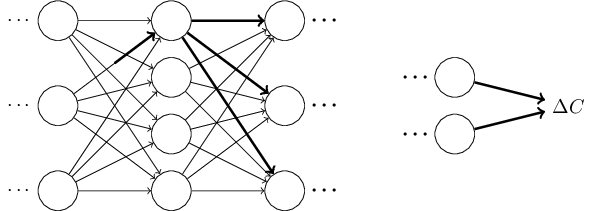
\includegraphics[width=.60\textwidth]{backProbError.png}
  \caption{The path how a change in one weight influences the loss function.\cite{Nielsen2015}
}\label{fig:backProbError}
\end{figure}
Equation \ref{eq:deltaC} shows how $\Delta C$ is related to $\Delta w^l_{jk}$
\begin{equation}\label{eq:deltaC}
\Delta C \approx \frac{\partial C}{\partial w^l_{jk}} \Delta w^l_{jk}
\end{equation}
where $l, j, k$ depict the $l^{th}$ layer, the $j^{th}$ neuron and the $k^{th}$ weight respectively.
The change invoked on the activation function is given by
\begin{equation}\label{eq:deltaA}
\Delta a^l_j \approx \frac{\partial a^l_j}{\partial w^l_{jk}} \Delta w^l_{jk}
\end{equation}
This change influences the next activation function as described in Equation \ref{eq:deltaA+}
\begin{equation}\label{eq:deltaA+}
\Delta a^{l+1}_q \approx \frac{\partial a^{l+1}_q }{\partial  a^l_j} \Delta  a^l_j
\end{equation}
Substituting from Equation \ref{eq:deltaA} leads to 
\begin{equation}\label{eq:deltaA++}
\Delta a^{l+1}_q \approx \frac{\partial a^{l+1}_q }{\partial  a^l_j}\frac{\partial a^l_j}{\partial w^l_{jk}} \Delta w^l_{jk} 
\end{equation}
The change in $\Delta a^{l+1}_q $ again causes change in the following layers. 
Imagining a path of activation $ a^l_j ,  a^{l+1}_q, \cdots, a^{L-1}_n, a^{L}_m$ the change in $\Delta C$ is given by
\begin{equation}\label{eq:deltaCfull}
\Delta C \approx \frac{\partial C}{\partial a^{L}_{m}} \frac{\partial a^{L}_{m}}{\partial a^{L-1}_{n}} \frac{\partial a^{L-1}_{n}}{\partial a^{L-2}_{p}} \cdots \frac{\partial a^{l+1}_{q}}{\partial a^{l}_{j}} \frac{\partial a^{l}_{j}}{\partial w^{l}_{jk}} \Delta  w^{l}_{jk}
\end{equation}
This only considers one path through the neural network, but to compute the gradient with respect to a certain weight all possible paths must be considered.
Equation \ref{eq:gradWRTw} shows how the change in one weight influences the loss function by the influence to all connected neurons and their respective activation functions.
\begin{equation}\label{eq:gradWRTw}
\frac{\partial C}{\partial w^{l}_{jk}} = \sum_{mnp \cdots q} \frac{\partial C}{\partial a^{L}_{m}} \frac{\partial a^{L}_{m}}{\partial a^{L-1}_{n}} \frac{\partial a^{L-1}_{n}}{\partial a^{L-2}_{p}} \cdots \frac{\partial a^{l+1}_{q}}{\partial a^{l}_{j}} \frac{\partial a^{l}_{j}}{\partial w^{l}_{jk}}
\end{equation}
This very intuitively shows how an error needs to propagated back through the network to optimize the loss by applying small changes to the weights with the use of gradient descent.
As explained earlier this technique relies highly on the loss surfaces and respectively the gradients. 
As the error propagates back through the NN by multiplication of the gradients it is easy to see that values can vanish if the multiplicators are rather small and will be multiplied often. 
This is called the \emph{vanishing gradient}
The opposite (\emph{exploding gradient}) happens if the gradient values are constantly bigger than $1$. 
This problem is easy to handle if values are limited by $1$.
In modern Frameworks like TensorFlow and Theano automatic differentiation(AD) is used which makes it easy to setup experimental DNNs without the need to explicitly differentiating activation and loss functions.\cite{ValdenegroToro2019DeepNN}


\subsection{Loss Function}\label{ssec:lossFunc}
As already seen in the preceding sections the \emph{Loss Function}(sometimes also referred to as \emph{Cost Function}) is an essential part in the Learning Process.
The loss function is a scalar function which reflects how "good" or "bad" predictions are in comparison with the \emph{Ground Truth}.
What "good" or "bad" means can strongly depend on the domain of the problem.
For different problems different loss functions are needed. 
In the following the four most important loss functions and it's applications will be discussed.
\paragraph{Mean Squared Error (MSE)}
The MSE is a very intuitive loss function which is defined by Equation \ref{eq:mse}.
\begin{equation}\label{eq:mse}
MSE(\hat{y}, y) = \frac{1}{n} \sum_{i = 0}^{n}(\hat{y}_i - y_i)^2
\end{equation}
The error between the prediction $\hat{y}$ and the label $y$ is defined by their difference, while the squaring helps producing only positive values. The MSE is also called $L_2$ loss because it is defined using the $L_2$ norm.
The MSE is typically used for regression tasks.
One problem with the MSE is that due to the square term,
large errors are penalized more heavily than smaller ones. This
produces a practical problem where using the MSE loss might lead
the convergence of the output to a mean of the ground truth values
instead of predicting values close to them.\cite{ValdenegroToro2019DeepNN}
\paragraph{Mean Absolute Error (MAE)}
The MAE or $L_1$ loss can get around this problem because it is given by
\begin{equation}
MAE(\hat{y}, y) = \frac{1}{n} \sum_{i = 0}^{n}|\hat{y}_i - y_i|
\end{equation}
The absolute error leads to the drawback that the MAE is not differentiable in it's origin.
The L1 loss can recover the median
of the targets, in contrast to the mean recovered by the L2 loss.\cite{ValdenegroToro2019DeepNN}
The MAE is like the MSE generally applied for regression tasks
\paragraph{Categorical Cross-Entropy (CCE)}
In classification a probability value $\hat{y}^c$ is given for every class $c$ in the classification domain $C$. 
CCE has proven to produce smoother loss surfaces for classification tasks and does not have the outlier weighting problem the MSE faces.
The CCE is defined as
\begin{equation}\label{eq:cce}
CCE(\hat{y}, y) = - \sum^n_{i = 0} \sum^C_{c = 0} y_i^c \mathrm{log} \hat{y}_i^c
\end{equation} 


\paragraph{Binary Cross-Entropy (BCE)}
For binary classification $\hat{y}$ is the probability of the positive class and Equation \ref{eq:cce} unfolds to 
\begin{equation}
BCE(\hat{y}, y) = - \sum^n_{i = 0} \left[ y_i \mathrm{log} \hat{y}_i + (1-y_i) \mathrm{log}(1-\hat{y}_i) \right]
\end{equation}

\subsection{Hyper-parameter Tuning}\label{ssec:hyperP}
What is the difference between parameters and \emph{hyper-parameters}?
The parameters are learned by the algorithm in the learning process and for ANNs they are normally referred to as the \emph{weights} of the ANN, whileas the \emph{hyper-parameters} will not be learned but need to decided by the human designer of the ANN or any other learning algorithm.
In the case of an ANN the hyper-parameters are for example the number of layers, the number of artificial neurons per layer, the type of neurons, the type of connection between layers, the learning rate for the optimizer, the batch size and the number of epochs to train the model.
The hyper-parameters basically decide if the model will be able to learn the implicit mapping given in the data.
\paragraph{Model complexity}
The model complexity is given by the number of parameters the learning algorithm needs to learn.
A model with too high complexity is prone to overfitting, while a model with too low complexity is prone to underfitting.
The goal is to find a model complexity, that perform very well on the training data but also generalizes to unseen data.
To achieve this kind of robustness \emph{regularization techniques} exist for basically any learning algorithm (see Section \ref{ssec:regularization}). 
\paragraph{Learning Rate}
As depicted in Figure \ref{fig:lr} the learning rate is very important for convergence. 
If the learning rate is to high the optimization process will fail by not finding the minimum but diverge around it.
On the other hand if the learning rate is to low convergence will happen but happens very slow. 
A good learning rate is crucial for fast convergence.
Typically learning rates in the range $[0, 1]$ are chosen, but it is common to take small values as negative power of 10 like $\alpha = [0.1, 0.01, 0.001]$.
The learning rate does not need to be static over the learning process and can be adjusted dynamically.
The typical
method is to decrease the LR by a factor after a plateau of the loss
curve has been detected, which potentially could allow the loss
to decrease further. \cite{ValdenegroToro2019DeepNN}
This can be imagined as throwing a ball in a loss surface which will roll in the lowest hollow. If it stops the ball will be changed for a smaller ball which will roll even lower in this hollow.
\paragraph{Batch Size}
As described in Section \ref{ssec:gradientDescent} the \emph{batch size} decides how many samples will be taken into account for one update of the MGD and that it is normally chosen as a power of two to efficiently use memory.
Bigger batches make a better approximation of the true gradient and decrease computation time but increase the memory needed for the computation.
The biggest possible batch size really depends on the model complexity but should be chosen to the maximum possible with given memory configurations.
\paragraph{Number of Epochs}
The \emph{number of epochs} decides about the length of training.
If this hyper-parameter is chosen too small the loss may have not converged at this time.
If it chosen to big training takes longer than needed and the risk of overfitting arises if no regularization means are used.
A way of getting a good compromise in an automated way is the early stopping criterion, which can monitor the validation loss or validation accuracy and stop if they are no longer decreasing or increasing respectively. 
This makes it possible to only set a reasonable minimum for the number of epochs.


\subsection{Over- / Underfitting}\label{ssec:overfitting}
The problem of \emph{overfitting} and \emph{underfitting} is as old as learning in general.
Overfitting happens if the model adjust too strong to the training data and therefore is no longer able to generalize to new data.
On the other hand underfitting is the complete opposite where the model generalizes to much so it can not properly map the real distribution of the data.
An intuitive example would be two students who learn for a test in a Chinese class but both aren't able to understand the language.
The test is multiple choice and they have some example tests for learning.

\textbf{Student A (the \emph{underfitter})} just looks at all the answers and realizes that most of the answers are in checkbox 2, so he decides to just tick checkbox two on every question. This leads to a bad score even in the example tests handed out for learning.

\textbf{Student B (the \emph{overfitter})} learns every question and the corresponding answers by heart which results in a perfect score in the example tests handed out for learning. If the final test includes the exact questions from the examples student B got lucky but if the questions and answers change their wording student B will perform poorly on the test. 

From a data perspective Figure \ref{fig:underfitting} - \ref{fig:overfitting} show how a linear regression underfitts with a polynomial degree of 0, while choosing a polynomial degree of 8 leads to overfitting.

\begin{figure}
\centering
  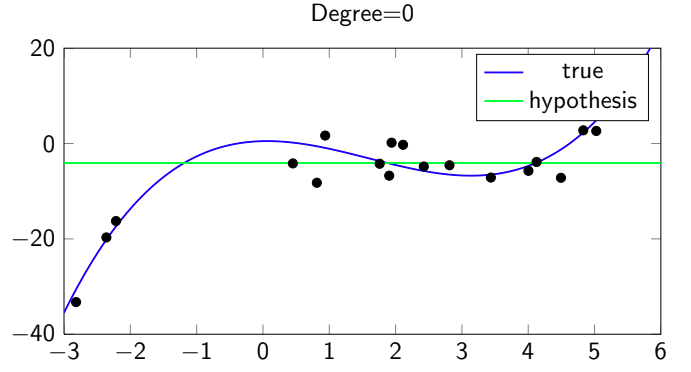
\includegraphics[width=.60\textwidth]{underfitting.png}
  \caption{The chosen model performs poorly even on the training data\cite{LVDFKI}
}\label{fig:underfitting}
\end{figure}

 \begin{figure}
\centering
  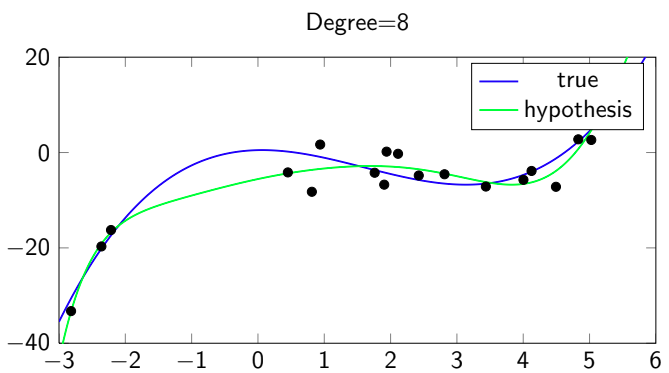
\includegraphics[width=.60\textwidth]{overfitting.png}
  \caption{The model performs very well on the training data but does not model the true function which is a polynominal with degree 3. \cite{LVDFKI}
}\label{fig:overfitting}
\end{figure}


\subsection{Regularization}\label{ssec:regularization}
Generally speaking regularization is a technique to prevent overfitting.
For the linear regression example in Figure \ref{fig:underfitting} - \ref{fig:overfitting} Tikhovnov regularization can be applied which penalizes large weights that are not supported by evidence from the data. This reduces the influence of higher polynomials(this variant of linear regression is called \emph{ridge regression}).
Although it is possible to apply Tikhovnov regularization(also called $L_2$ regularization) deep learning techniques like \emph{Dropout} and \emph{Batch Normalization} have proven to work very well while being easy to implement.
\paragraph{Dropout}
Dropout randomly removes neurons from the network for each iteration. 
This simple step simulates training a large number of NNs with slightly different model structures in parallel.
Figure \ref{fig:dropout} depicts one possible randomly chosen model structure.

 \begin{figure}
\centering
  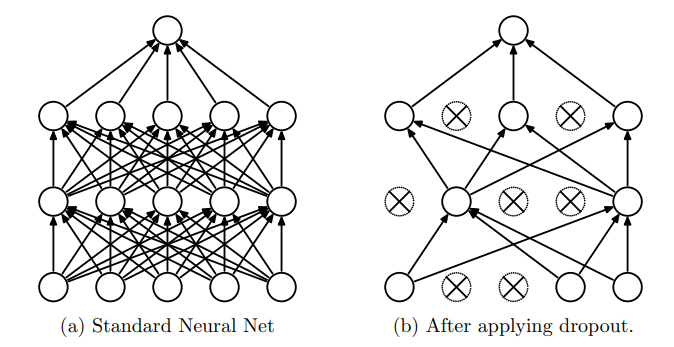
\includegraphics[width=.60\textwidth]{dropout.png}
  \caption{Dropout Neural Net Model. \textbf{Left:} A standard neural net with 2 hidden layers. \textbf{Right:}
An example of a thinned net produced by applying dropout to the network on the left.
Crossed units have been dropped. \cite{JMLR:v15:srivastava14a}
}\label{fig:dropout}
\end{figure}

Srivastava et al. figured that \emph{units may change in a way that they fix up the mistakes of the other units. This may lead to complex co-adaptations. This in turn leads to overfitting because these co-adaptations do not generalize to unseen data.}\cite{JMLR:v15:srivastava14a}
The suggested solution to break up the co-adaptions was to introduce noise in the form of a mask $\mathbf{m}$ of length n.
Every entry in this mask is either $0$ or $1$ with a probability $p$ to be $1$.
The \emph{dropout layer} can be imagined as a layer that cuts some connections (multiplication with $0$) and lets some of the connections through (multiplication with $1$). 
This mask is ordered new in every iteration, meaning the neurons that will be cut off will change in every iteration.
While neurons will be dropped during training this is not the case for inference or testing. To account the for the absence of $(1-p)\%$ of the neurons during the training all activation functions will be multiplied by $p$.
Srivastava et al. showed in Figure \ref{fig:dropoutResults} that using dropout layers invokes an increase in the robustness of several DNNs and therefore decreases the classification error of those DNNs drastically.

 \begin{figure}
\centering
  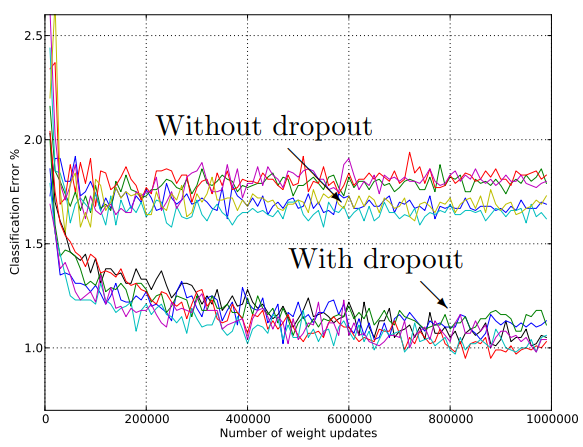
\includegraphics[width=.60\textwidth]{dropoutResults.png}
  \caption{Test error for different architectures
with and without dropout. The networks have 2 to 4 hidden layers each
with 1024 to 2048 units. \cite{JMLR:v15:srivastava14a}
}\label{fig:dropoutResults}
\end{figure}

\paragraph{Batch Normalization}
%die verteilung des inputs eines layers ändert sich andaurnd während des trainings, weil die gewichte der vorherigen layer angepasst werden. Das verlangsamt das training und wird s internal covariate shif gennannt. Jeder eingehende batch wird normalisiert, was diesen Effekt veringert und dadurch Lernen schneller machen kann. Liegt wahrscheinlich auch daran, dass die loss surface smoother ist.
Batch normalization is a technique developed to enhance the training speed but has the nice side effect of regularizing quite well.
The general idea Sergey Ioffe et al. where pursuing in \cite{ioffe2015batch} was to reduce \emph{internal covariate
shift}. \emph{internal covariate
shift} is described as the phenomenon that the distribution of each layer's input is changing during training due to the adaption of weights.
\emph{ The
intuition for Batch Normalization is that drastic internal covariate
shift is prejudicial for neural network training, as it is more likely to saturate non-linearities, and unstable activation distributions
will need more training iterations to converge successfully. Both
situations causes slow training convergence.}\cite{ValdenegroToro2019DeepNN}
The normalization is performed component-wise on the features, so that features have a mean of $0$ and a standard deviation of $1$.
The mean of a batch is given by
\begin{equation}
\mu_B = \frac{1}{|B|} \sum_{i=0}^m x_i
\end{equation}
and the variance of the batch is given by
\begin{equation}
\sigma^2_B = \frac{1}{|B|} \sum_{i=0}^m (x_i - \mu_B )^2
\end{equation}
The normalized features of the batch are then defined as
\begin{equation}
\hat{x}_i = \frac{x_i - \mu_B}{\sqrt{\sigma^2_B + \epsilon}}
\end{equation}
where the batch $B = {x_0, \cdots, x_m}$,  $|B|$ is the size of the batch and $\epsilon = 0.001$ is a very small constant to prevent division by zero.
The scaled shift is applied by
\begin{equation}
y_i = \gamma \hat{x}_i + \beta
\end{equation}
where $\gamma$ and $\beta$ are parameters that need to learned.
Batch normalization is a very stable technique with basically no drawbacks, that is why it is used by most modern NN architectures (for example ResNet, GoogleNet and DenseNet use it).
Shibani Santurkar et al. show in \cite{2018arXiv180511604S} that batch normalization smoothes the loss surface and therefore achieves the regularization effect.

\subsection{Convolutional Layers}\label{ssec:Conv}
A convolutional layer is a layers in a NN in which the artificial neuron described earlier are replaced with a filter(sometime also referred to as kernel).
The \emph{convolutional layer} has its name because these filters perform convolution on the input data.
\subsubsection{Convolution}\label{ssec:convolution}
Mathematically speaking \emph{convolution} is expressing how the shape of one function modifies the other and is defined by
\begin{equation}\label{eq:convolution}
(f * g) = \int_{\mathbb{R}^n} f(\tau)g(x-\tau)\mathrm{d}\tau
\end{equation}
Because Equation \ref{eq:convolution} may not be very intuitive the following example will show convolution on an image, because that is what it is used for in CNNs.
An image can be imagined as a 2-dimensional discrete function $f: \mathbb{Z}^{W \times H}  \rightarrow \mathbb{Z}^Z$ which maps every $(x,y)$ position to a pixel value $z$.
Where $W$ denotes the \emph{width}, $H$ the \emph{height} and $Z$ the pixel value.
If a grayscale image is considered $z \in [0, 255]$(the range $[0, 255]$ is internally often represented as the range $[0, 1]$).
Now the second function is needed and this is the filter. 
A filter $\omega: \mathbb{Z}^{M \times N}  \rightarrow \mathbb{R}$ is a 2-dimensional discrete function which describes how each pixel will be influenced by its neighboring pixels. Although filters can have different dimensions for $N$ and $M$ they are normally designed as being quadratic.
Figure \ref{fig:filter} shows the results of convolving a filter designed to detect edges on a small sample image.
\begin{figure}
\centering
  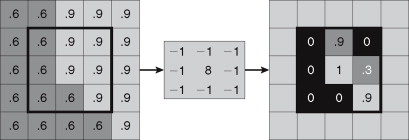
\includegraphics[width=.80\textwidth]{edgeDetection.jpg}
  \caption{3 x 3 filter for edge detection applied on small sample image \cite{BRINKMANN200893}
}\label{fig:filter}
\end{figure}
Applying the filter is done by calculating a weighted average for every pixel in the image therefore the filter is shifted over the whole image.
This is defined by
\begin{equation}
g(x,y) = \omega * f(x,y) = \sum_{s=\left \lceil-M/2 \right \rceil}^M \sum_{s=\left \lceil-N/2 \right \rceil}^N \omega(s, t)f(x-s, y-t)
\end{equation}\label{eq:filter}
The definition in Equation \ref{eq:filter} assumes that the summation point for the filter is in $\omega(0,0)$ and the positions within the filter range from $[\left \lceil-M/2 \right \rceil, \left \lfloor M/2 \right \rfloor]$ and $[\left \lceil-N/2 \right \rceil, \left \lfloor N/2 \right \rfloor]$ respectively, which also implies that the \emph{width} $M$ and the \emph{height} $N$ of the filter must be odd values.
For the given example in Figure \ref{fig:filter} starting from the upper left corner this leads to $g(1,1) = 0.6 * (-1) + 0.6 * (-1) + 0.9 * (-1) + 0.6 * (-1) + 0.6 * (8) + 0.9 * (-1) + 0.6 * (-1) + 0.6 * (-1) + 0.9 * (-1) = -0.9 $, which will be clipped to the domain of $[0,1]$ resulting in $g(1,1) = 0$.
Then the filter will be shifted one step to the right which leads to $g(2,1) = 0.6 * (-1) + 0.9 * (-1) + 0.9 * (-1) + 0.6 * (-1) + 0.9 * (8) + 0.9 * (-1) + 0.6 * (-1) + 0.9 * (-1) + 0.9 * (-1) = 0.9$. This is performed for the whole image until it leads to the output depicted in Figure \ref{fig:filter}.
Filters with different weights have different functions.
While the filter in the given example is used for edge detection different configurations can be used for blurring, sharpening and many other applications. 
A convolutional layers is constructed from multiple filters and the output of it is given by

\begin{equation}
\mathbf{y}= f(\mathbf{x} * \mathbf{F} + b)
\end{equation},
where $\mathbf{x}$ is the input image, $\mathbf{F}$ is the filter, $b$ is the bias and $f$ is the activation function.
For every filter in the layer a new image is created. 
These images are called \emph{convolutional feature map}, because they represent specific visual features extracted by the filter(for example edges).
The filter weights and biases in a convolutional layer are not set like in the edge detection example, but are learned while performing gradient descent.
\subsubsection{Convolutional Neural Networks (CNNs)}\label{ssec:convNets}
As described in Section \ref{ssec:Conv} convolutional filters can be trained to detect specific features in images.
These features have the big advantage that they can be calculated position independent.
If processing an image with a NN with classical neurons every neuron would be connected to a pixel and therefore could only make sense for that specific pixel.
For image classification this would mean the classification of a specific object in an image can only be made if the object will always be in the same place. This is not very helpful.
As explained filters go over the whole image and calculate a new image with respect to a certain feature.
A CNN which classifies letters would most certainly learn filters for horizontal, vertical and different diagonal edges and some more for different types of corners in its first layer.
The followings layer would learn filters as some combination of those. An "A" for example consists of two diagonal lines and a horizontal line and it does not matter where in the image the structure appears it only matters that the features(lines and edges in this case) are in the same constellation.
If the aim is to classify more complex structures it is important to account the hierarchy of features.
The combination of features like edges and corners will take place on a bigger scale.
Therefore either the filters on the following layer need to be bigger or the resulting feature map needs to be down sampled.
The latter is called \emph{Pooling} and is for reasons of performance and memory efficiency the preferred solution.
The parameters the CNN would need to learn with enlarging the filters would grow exponentially.
On top of the convolutional layers a dense layer is needed to make the classification. 
With this being connected to a very big convolutional feature map resulting from a CNN without pooling the dense layer becomes very big and is therefore prone to overfitting.
Pooling can be performed using a $M \times M$ grid and shifting it over the feature map with a step size of $M$. For every step the maximum(for Max-Pooling) or the average(for Average-Pooling) is calculated. 
These new values represent the the down sampled feature map. 
The down sampling is performed by the rate $M^{-2}$.

CNNs have proven to be state of the art in image classification tasks since in 2012 the AlexNet was winning the Large Scale Visual Recognition Challenge (ILSVRC) \cite{ILSVRC} competition with a top-5 test error rate of 15.3\%,
compared to 26.2\% achieved by the second-best entry.\cite{NIPS2012_4824}
So today CNNs have become the standard for NNs and images but they are also used for sound related learning tasks like voice recognition or speaker identification.
This is the case because a sound signal can be fully represented as an image of a sound wave.
CNNs perform good on data where features close to each other also have a close relation between each other.
Images obviously comply with this rule, because if all pixels of an image would be shuffled all information would be lost.
\subsection{Recurrent Layers}
All NNs described before are \emph{feedforward neural networks}.
That means that information is passing the network only from input towards output.
Feedforward NNs are working very well for a lot of problem settings but they are not able to save an internal state.
The human brain in contrast processes information in sequence and produces an internal model of prior processed information, which continuously changes by the influence of new input.
Reading for example takes as input one word at a time and produces an internal model of the text.
In the "real world" everything is attached to the time and therefore this applies to every aspect of learning in the human brain. 
In data science it is a common practice to only consider data at a specific point in time, which makes it possible to use feedforward NNs for a wide variety of tasks.
But if a temporal relation needs to be modeled Recurrent Neural Networks(RNNs) are the approach to model these time dependent tasks.

Figure \ref{fig:RNN} shows that RNNs use loops to use the output of a recurrent layer as part of its input. 
This behavior is defined by
\begin{equation}
\mathbf{h}^{(t)} = f(\mathbf{h}^{(t-1)}, \mathbf{x}^{(t)}; \mathbf{\theta})  
\end{equation}\label{eq:RNN}
where $\mathbf{h}^{(t)}$ is the state at time $t$ and $f$ a function that calculates the state $\mathbf{h}^{(t)}$ from the state $\mathbf{h}^{(t-1)}$ at time $t-1$ and the input $\mathbf{x}^{(t)}$ at time $t$ and a given set of parameters $\theta$.
\begin{figure}
\centering
  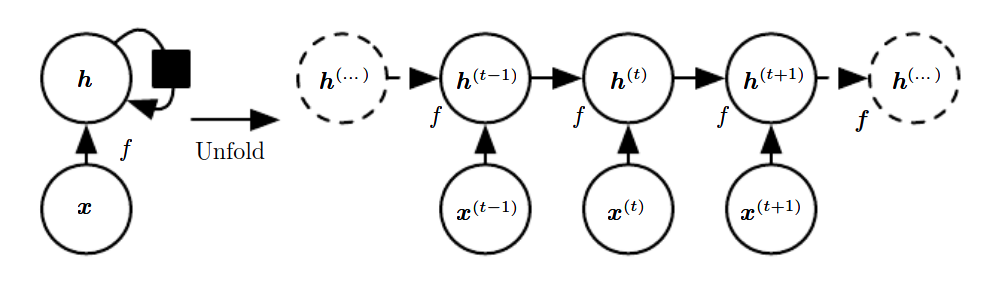
\includegraphics[width=.75\textwidth]{RNN.png}
  \caption{A recurrent network with no outputs. This recurrent network just processes information from the input $\mathbf{x}$ by incorporating it into the state $\mathbf{h}$ that is passed forward through time. (Left) Circuit diagram. The black square indicates a delay of a single timestep. (Right) The same network seen as an unfolded computational graph, where each node is now associated with one particular time instance. \cite{Goodfellow-et-al-2016}
}\label{fig:RNN}
\end{figure}
Figure \ref{fig:RNNLearn} shows how learning is applied to the given structure with labels $\mathbf{y}$, outputs $\mathbf{o}$ and a loss function $L$.
\begin{figure}
\centering
  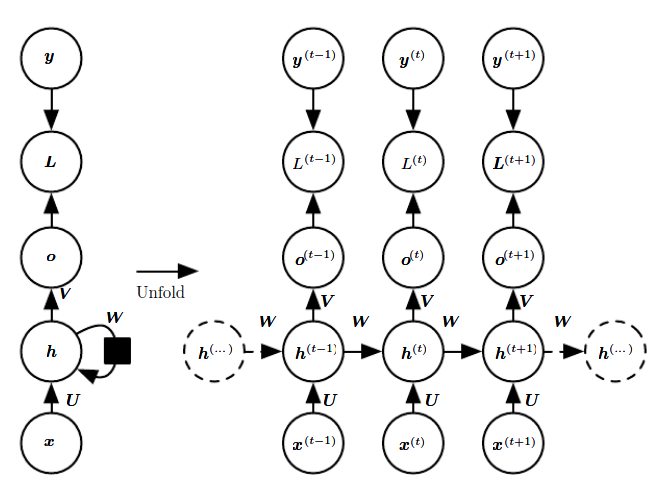
\includegraphics[width=.75\textwidth]{RNNLearn.png}
  \caption{The computational graph to compute the training loss of a  recurrent 
  network that maps an input sequence of 
$\mathbf{x}$ 
 values to a corresponding sequence of output $\mathbf{o}$ values. A loss $L$ measures how far each $\mathbf{o}$ is from the corresponding training target $\mathbf{y}$. When using softmax outputs, we assume $\mathbf{o}$ is the unnormalized log probabilities. The loss $L$ internally computes $\hat{y}=softmax(\mathbf{o})$ and compares this to the target $\mathbf{y}$. The RNN has input to hidden connections parametrized by a weight matrix $\mathbf{U}$, hidden-to-hidden recurrent connectionsparametrized by a weight matrix $\mathbf{W}$, and hidden-to-output connections parametrizedby a weight matrix $\mathbf{V}$.(Left) The RNN and its loss drawn with recurrent connections. (Right) The same seen as a time-unfolded computational graph, where each node is now associated with one particular time instance. \cite{Goodfellow-et-al-2016}
}\label{fig:RNNLearn}
\end{figure}


\subsection{Long Short-Term Memory (LSTM)}\label{ssec:LSTM}
The classical RNN structure suffers from the problem of the vanishing gradient.
Sepp Hochreiter and Jürgen Schmidhuber proposed a solution to that problem in \cite{LSTM}.
The proposed architecture is called Long Short-Term Memory(LSTM) and introduces a short-term memory that is able to learn on time series of over 1000 discrete timesteps.
Figure \ref{fig:LSTMFig} shows that the LSTM comes with \emph{input, output, forget gate} to control input and output of the cell.

\begin{figure}
\centering
  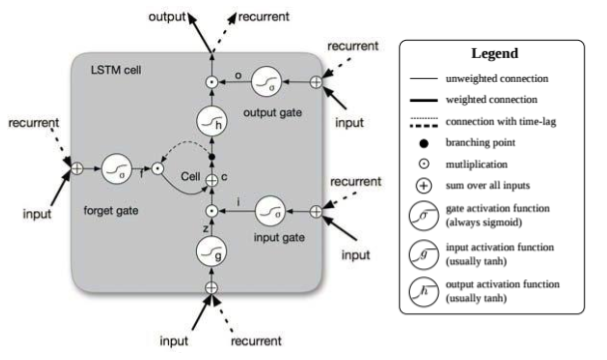
\includegraphics[width=.90\textwidth]{LSTMFig.png}
  \caption{Detailed schematic of a Long Short-Term Memory cell \cite{LSTMFig}
}\label{fig:LSTMFig}
\end{figure}

These gates have very descriptive names.
The input gate controls if(or better when) input is taken into consideration to update the internal state.
The output gates controls the output in the same way, whileas the forget gate controls when the internal state should be reset and when it should be sustained.
If the forget gate sustains the state of the cell the state will always be added to the activated and gated input in the next step.
Hochreiter and Schmidhuber called this internal time shifted addition the \emph{Constant Error Carrousels}(CEC).
The addition in the CEC prevents the problem of the vanishing gradient.
While feed forward networks can only be used to make a one to one prediction, LSTMs(and other RNN structures) can be used for different types of predictions.
\paragraph{one to many} predictions take a single input and produce a sequence of outputs.
This can find application in captions for images where the caption can be a sentence of a variable length.
In this case the output gate controls how the sequence of words will be shaped. 
For example an image showing a dog chasing a ball should be described as "Dog chasing ball" but not as "Ball chasing dog" although the same words are used.
The weights of the output gates of the LSTM layer in this case implicitly know about the structure of a sentence and the meaning of the words and how they make sense.
\paragraph{many to one} prediction work with a sequence as input and produce a single output.
This is how predictions for the VVAD are working. The NN takes a sequence of features(face images, lip images, facial features or lip features) as input and predicts if this sequence is a positive \emph{speaking} or a negative \emph{not speaking} sample.
Here the input gate learns which timesteps of the input data should be considered to update the internal state.
\paragraph{many to many} or \emph{sequence to sequence} predictions use a sequence as input data and produce a sequence as output. 
This can be used to extend the image caption example to video captions. Another application is speech recognition where voice(a sequence of frequencies) is taken as input to predict a sequence of words.

%TODO feature extraction am besten in convNets kurz erklären

%TODO Metrics https://towardsdatascience.com/metrics-to-evaluate-your-machine-learning-algorithm-f10ba6e38234 (Bonus)



 
%TODO data augemtation(Bonus)


\chapter{The Data}
\label{cha:data}
As Markus Schmitt states in \cite{Schmitt2018} that the data is one of the most important if not the most important
factor in a machine learning project, for this reason we will take a deeper look into our data.
In the following chapter we present
the LRS3 dataset (described in Section \ref{sec:lrs3}) we use to construct the VVAD dataset (described in Section \ref{sec:vvadData}).
How we extract positive and negative samples from it is described in Section \ref{ssec:dataAcquisition}.
Section \ref{ssec:dataPreprocessing} covers the necessary steps in the preprocessing.
In general one has to distinguish between the training data and the test data. While the training data is
used to train the chosen machine learning algorithm, the test data is used to evaluate how good the algorithm performs.
The construction of the test set is described in Section \ref{ssec:testset}.
A general description what data needs to fulfill in order to be learnable and how to split data into training, validation and test set is given in Section \ref{ssec:dataTheory}
The results and how the evaluation is performed is presented in Chapter \ref{cha:eval}.

\section{Lip Reading Sentences 3 (LRS3) Dataset}\label{sec:lrs3}
Since the VVAD is implemented with a learning algorithm, to reduce the false positive rate, which is relatively high in the classic approach of lip motion detection (see Section \ref{sec:relatedWorks}).
The learning algorithm should be able to distinguish between a natural lip motion in \emph{ not speaking} phases and the lip motion which is associated with \emph{speaking} phases.
To accomplish that a dataset with a large amount of natural \emph{speaking} and \emph{not speaking} scenarios is needed.
Triantafyllos Afouras et al. introduced in \cite{Chung18} a large-scale dataset for visual speech recognition from videos of 5594 TED and TEDx talks.
It provides more than 400 hours video material of natural speech.
Which is substantially more compared to other
public datasets that are available for general research.
A comparison of datasets is shown in figure \ref{fig:datasetCompare}.

\begin{figure}
  \centering
  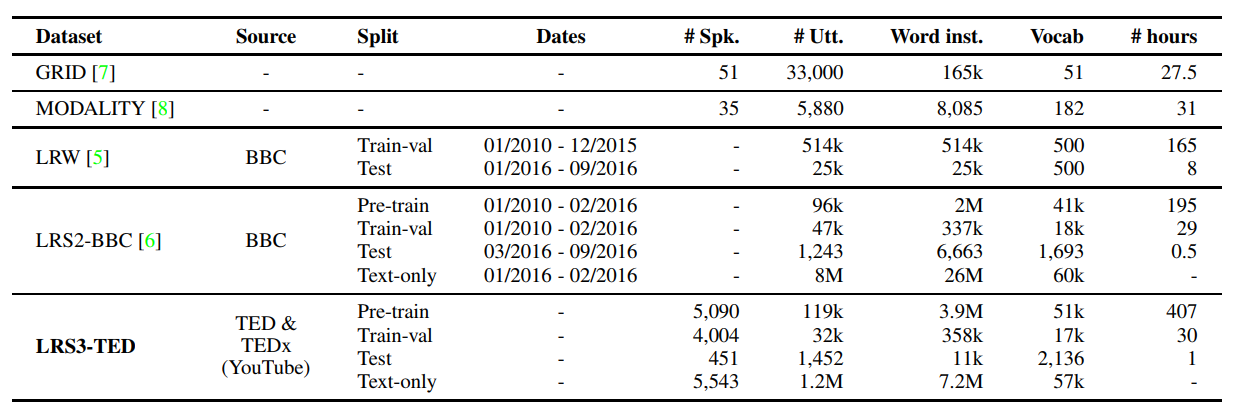
\includegraphics[width=.95\textwidth]{datasetCompare.png}
  \caption{A comparison of publicly available lip reading datasets. Division of training, validation and test data; and the number of utterances, number
of word instances and vocabulary size of each partition. Utt: Utterances.\cite{Chung18}}
  \label{fig:datasetCompare}
\end{figure}

The LRS3 dataset provides videos of TED and TEDx talks along with text files containing information about the position of the face and the said words.
In the text file the following fields are important for the transformation to the VVAD dataset (An example of a LRS3 sample can be found in Appendix \ref{app:dataSample}):
\paragraph{Text} contains the text for one sample. The length of the text or respectively the sample is defined by length of the scene. 
That means one sample can get as long as the face is present in the video.
\paragraph{Ref} is the reference to the corresponding YouTube video. The value of this field needs to be appended to \texttt{https://www.youtube.com/watch?v=}
\paragraph{FRAME} corresponds to the face bounding box for every frame, where \texttt{FRAME} is the frame number, \texttt{X} and \texttt{Y} is the position of the bounding box in the video and \texttt{W} and \texttt{H} are the width and height of the bounding box respectively. It is to mention that for the frame number a frame rate of 25 fps is assumed and the values for \texttt{X}, \texttt{Y}, \texttt{W} and \texttt{H} are a percentage indication of the width and height of the video.
\paragraph{WORD} maps a timing to every said word. Here \texttt{START} and \texttt{END} indicate the start and end of the word in seconds respectively. 
It is to mention that the time is in respect to the start of the sample given by the first frame and not to the start of the whole video.
\paragraph{}%Pseudo end

The LRS3 dataset comes with a very low bias towards specific ethnic groups, because TED and TEDx talks are international and talks are held by men and women as well as by kids. 
It also comes with the advantage that it depicts a huge variety of people because the likelihood of talking in multiple TED or TEDx talks is rather small.
This is a big advantage over the LRS2 and LRW dataset that are extracted from regular TV shows, which brings the risk of overfitting to a specific persons. 
LRS3 makes learning more robust in that sense. 
Since natural speech in front of an audience includes pauses for applause and means to structure and control a speech as described in \cite{Nikitina2011}, the LRS3 dataset provides \emph{speaking} and \emph{not speaking} phases.
How we extracted the positive (\emph{speaking}) and negative (\emph{not speaking}) samples from the LRS3 dataset is described in Section \ref{ssec:dataAcquisition}.


\section{VVAD Dataset}\label{sec:vvadData}
From the LRS3 dataset described in Section \ref{sec:lrs3} a new dataset is constructed.
The newly created dataset will be call VVAD dataset.
The close relation between lipreading and VVAD makes it possible to adjust the LRS3 to be used for the purpose of Visual Voice Activity Detection
The VVAD dataset is created by an automated process depicted in Section \ref{sec:createVVAD}.
The produced VVAD dataset comes in four different flavors for the samples.
These flavors are related to the four different learning approaches described in Section \ref{ssec:algorithm} and are visualized in Figure \ref{fig:flavors}.
\paragraph{Face Images} used for the most sophisticated model.
These Face Images come in a maximal resolution of $200 \times 200$ pixels and with a maximal number of 38 frames.
So the maximal shape of one sample of the flavor \emph{Face Images} is $38 frames \times 200 pixels \times 200 pixels \times 3 channels = 4560000$.
Face Images are RGB images, so the 3 channels correspond to the 3 RGB channels.
Pixel values range between 0 and 255 which can be represented with one byte. 
This means one \emph{Face Images} sample takes 4560000 bytes, which equals $4.56$ mega bytes.
\paragraph{Lip Images} are also used for an End-to-End learning approach but they obviously concentrate on a small subset of the Face Images.
As well as the Face Images, the Lip Images are RGB images coming with a maximum of 38 frames but they have a maximal resolution of $100 \times 50$ pixels.
This resolves to a size of $0.57$ mega bytes given by $38 frames \times 100 pixels \times 50 pixels \times 3 channels = 570000$
\paragraph{Face Features} are used for the learning approach which focuses on facial features. 
These facial features are landmarks extracted from dlib's facial landmark detector 
as described in Section \ref{sec:createVVAD}.
It provides 68 landmarks with a (X,Y)-Position for a single face as depicted in Figure 
\ref{fig:shape}.
A single feature is given as float64 (8 bytes), resulting in a size of $41.344$ kilo bytes, given by $38 frames \times 68 features \times 2 \times 8 bytes = 41344$.
\paragraph{Lip Features} are a small subset of Face Features that only take the features of the lips into account. 
Dlib's facial landmark detector
reserves 20 features for the lips as shown in Figure \ref{fig:shape}.
This results in the size of $38 frames \times 20 features \times 2 \times 8 bytes = 12160$ for a single sample in the lip features flavor.

\begin{figure}
\centering
\parbox{\textwidth}{
\begin{subfigure}{.5\textwidth}
  \centering
  \captionsetup{width=.8\linewidth}
  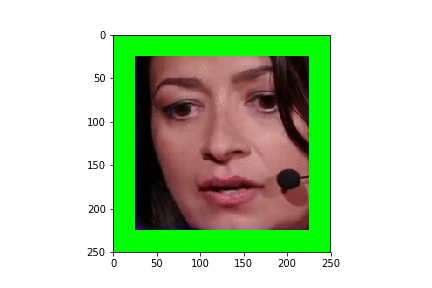
\includegraphics[width=\linewidth]{faceImages.png}
  \caption{Visualization of one frame in \emph{Face Images} flavor}
\end{subfigure}%
\begin{subfigure}{.5\textwidth}
  \centering
  \captionsetup{width=.8\linewidth}
  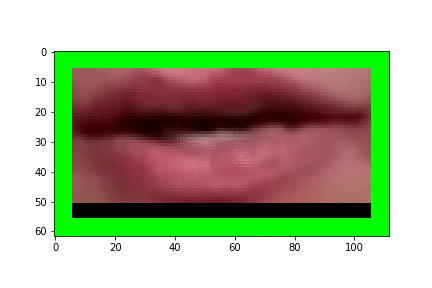
\includegraphics[width=\linewidth]{lipImages.png}
  \caption{Visualization of one frame in \emph{Lip Images} flavor}
\end{subfigure}
}
\parbox{\textwidth}{
\begin{subfigure}{.5\textwidth}
  \centering
  \captionsetup{width=.8\linewidth}
  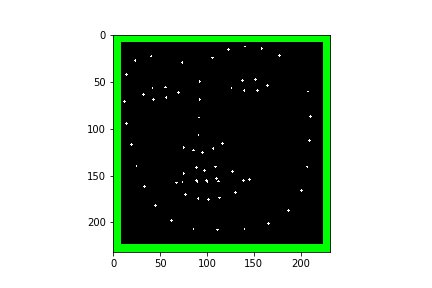
\includegraphics[width=\linewidth]{faceFeatures.png}
  \caption{Visualization of one frame in \emph{Face Features} flavor}
\end{subfigure}%
\begin{subfigure}{.5\textwidth}
  \centering
  \captionsetup{width=.8\linewidth}
  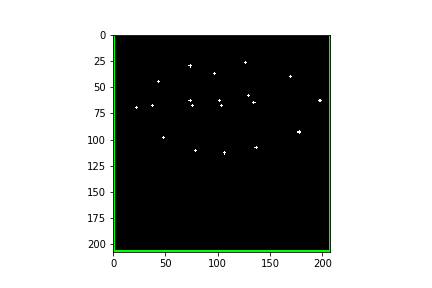
\includegraphics[width=\linewidth]{lipFeatures.png}
  \caption{Visualization of one frame in \emph{Lip Features} flavor}
\end{subfigure}%
}
\caption{Visualization for the different flavors.}
\label{fig:flavors}
\end{figure}

As the VVAD dataset is designed for binary classification it provides two classes.
The positive class in this case is \emph{speaking}, while the negative class is \emph{not speaking}. This holds for all the different flavors and takes one byte per sample.
The VVAD dataset comes with 44,289
samples equally distributed to the classes (22,144 
positive samples and 22,145 
negative samples) for training and validation set.
The total size of the VVAD dataset in bytes can be calculated with $(|S| + 1) \times |D|$, where $|S|$ is the size of one sample and $|D|$ the total number of samples in the dataset. 
The size of the sample is incremented by one because the label for every sample takes another byte.
This results in the following total sizes for the different flavors:
\begin{itemize}
\item[•] \textbf{Face Images:} $(4,560,000 + 1) bytes \times 44,289 = 201,957,884,289 bytes \approx 201.96 GB $ 
\item[•] \textbf{Lip Images:} $(570,000 + 1) bytes \times 44,289 = 25,244,774,289 bytes \approx 25.24 GB $ 
\item[•] \textbf{Face Features:} $(41,344 + 1) bytes \times 44,289 = 1,831,128,705 bytes \approx 1.83 GB $ 
\item[•] \textbf{Lip Features:} $(12,160 + 1) bytes \times 44,289 = 538,598,529 bytes \approx 538.6 MB $ 
\end{itemize}
Although it would be possible to construct a larger dataset it was chosen to create a balanced dataset.
This means all classes in the data are equally distributed.
An imbalanced dataset impose the danger of the learning algorithm taking shortcuts.
Imagining a very imbalanced binary dataset which has 90\% positive samples and 10\% negative samples.
The problem here is that learning is basically an optimization process, which aims to minimize a loss function.
If the loss function is just measuring how good the output matches the input over all samples it is obvious that the output will be optimized to show the positive class.
If the validation set has the same distribution as the training set this will give a accuracy of 90\%.
Which seems to be pretty good on first sight but if a closer look is taken the classifier unfolds to classifying everything as positive because it works for most of the samples.
There are techniques like undersampling, oversampling, synthetic data generation and cost sensitive learning to prevent this problem which will not be discussed any further because the easiest solution is to create a balanced dataset.
The creation of a balanced dataset is not always possible but as described in Section \ref{ssec:dataAnalysis} it is possible for the VVAD dataset.


\subsection{Test Set}\label{ssec:testset}
As described in Section \ref{ssec:VVADHACL} a human accuracy level test is performed on a small representative subset of 200 samples.
These 200 samples will be used as the test set to ensure the comparability between the results of the developed VVAD and the human accuracy level empirically determined by the human accuracy level test.
The test set contains the same samples for every flavor and can be used to verify the accuracy for the different learning approaches.




\section{Potential Problems with Big Data}\label{sec:problemsBigData}
The National Institute of Standards and Technology (NIST) defines Big Data the following: 
\begin{quote}
\textit{Big Data consists of extensive datasets - primarily in the characteristics of volume, variety, velocity, and/or
variability - that require a scalable architecture for efficient storage, manipulation, and analysis.}\cite{NIST2018}
\end{quote}
In general when we look at the complexity of an algorithm two aspects should be considered. The first aspect is the amount of processing time the algorithm needs. The other aspect is the amount of space or memory the algorithm needs. Memory is primary considered as RAM (Random-Access Memory) but when it comes to Big Data one also needs to consider the space a dataset takes on hard drive. 
If you don't have infinite time and space, which you never have, you want to optimize your algorithm in one direction or find a compromise between both aspects.

In relation to the datasets described in Section \ref{sec:lrs3}-\ref{sec:vvadData} and the data acquisition described in \ref{ssec:dataAcquisition} this leads to some potential problems, which will be discussed in the following.
On the hardware used to produce the VVAD dataset there is a 1.5 TB hard drive designated for data. 
The original downloaded LRS3 dataset takes approximately 500 GB, leaving 1 TB for datasets constructed via the proposed data acquisition. 
At this point the first problem arises: How to save the constructed dataset? 
As described in \ref{ssec:dataAcquisition} a sample consists out of \texttt{k} frames of features, which can of pixels or facial features extracted from an image and a positive or negative label. 
Space efficient would be to get the samples from the encoded videos every time they are needed for a training of the algorithm.
This is not an in-depth definition of encoding, but what it basically does is to save the difference between to frames, which is in a video very little, so it saves a lot of space but needs a little more time to calculate the next frame from the previous. On the other hand saving the raw frames is time efficient put costs more space.
So getting the sample directly from the video is space efficient because no extra space is needed to save the newly constructed samples.
But the following example shows that this is highly time inefficient.
Experiments have shown that it takes approximately 1143.856 s to get 100 samples from the videos, while it takes only 0.127 s to get 100 previously saved samples from the hard drive. This is more than 9000 times faster. Knowing 900 thousand samples can be produced from the LRS3 dataset it will take approximately 120 days to get all samples. With the hardware used to produce the VVAD dataset it is possible to parallelize the process in 12 cores. 
To implement this parallel processing of the videos the producer-consumer patterns was applied. 
12 producer run in parallel to produces samples from videos while one consumer saves these samples in a given ratio to the hard drive. This shrinks the time to produce a dataset to around 10 days. This is suitable for doing it once but not for every training considering there is a process of tuning the parameters, which takes multiple training sessions to complete. 
On the one hand it is obvious that it is not suitable to get the samples from the videos for every training, on the other hand the space this newly constructed dataset consumes needs to be determined.  
Assuming a sample with a \texttt{sampleLength} of 1.5 seconds and a shape of $200\times200$ pixels, the sample consumes approximately 4.5 MB. Figure \ref{fig:sampleDistribution} shows that with the given \texttt{sampleLength} a total number of over 900 thousand samples can be constructed. Applying that to the 4.5 MB, the constructed dataset will take approximately 4 TB. This space is not available on the hardware used to produce the VVAD dataset.
Here the first problem arises which needs to be solved implementing a compromise. 
The analysis of the data shows that for the purpose of the VVAD only a very imbalanced dataset can be constructed (see Figure \ref{fig:sampleDistribution}), knowing that it is possible to reduce the size needed by only saving a balanced dataset. 
This makes sense from a perspective of capacity, in Section \ref{sec:vvadData}
it is described why it makes sense to under-/oversample to a balanced dataset from a learning perspective.
Saving a dataset with a positive-to-negative-ratio of 1 to 1 instead of 30 to 1 needs approximately 266 GB.

\chapter{The Implementation}

\section{Creating the VVAD Dataset}\label{sec:createVVAD}

\subsection{Data Acquisition}\label{ssec:dataAcquisition}
The dataset described in section \ref{sec:lrs3} is designed for visual speech recognition. It holds over 100 thousand samples containing a video, a face bounding box and the timing of the said words.
From this we want to go to a dataset containing samples consisting of \texttt{k} frames of features (facial features or pixels) and the corresponding label (\emph{speaking} or \emph{not speaking}).

To access the LRS3 one needs to download the corresponding TED and TEDx talks from YouTube and make sure the frame rate is adjusted to what is used in the LRS3. To download the talks from YouTube and adjust the frame rate to 25 fps a python script was written. The resulting LRS3 dataset with the corresponding videos consumes round about 500 GB.

\subsubsection{Data Analysis}\label{ssec:dataAnalysis} 
Before using data to train an algorithm or transform the data to a specific dataset one should analyze the data to get the most out of it.

Visual speech recognition is slightly different to VVAD in the definition of distinguishable classes.
While a VVAD is a binary classification problem with the two classes \emph{speaking} and \emph{not speaking}, visual speech recognition is a multiclass classification problem.
VVAD can be seen as a level below visual speech recognition, since it only detects if someone is speaking or not and doesn't include any assumptions about the content of speech.
Therefore to use the LRS3 dataset we need to alter the labels from words to \emph{speaking} or \emph{not speaking}.
To do so we introduce a pipeline that detects pauses in the given speech sample.
In \cite{BrigPaus1994} Brigitte Zellner
shows that pauses occur in natural speech and explicitly in speech in front of an audience.
This leads to two constants we need to define in the context of pauses.
The first is \texttt{maxPauseLength} which defines the maximal length of a pause which is still considered to be an inter speech pause.
There are different classes of inter speech pauses.

— \emph{Intra-segmental pauses} are those which are related to the occlusions
of the vocal tract in normal speech production.
This kind of pauses are up to $100ms$ long and are not recorded in the LRS3 dataset, because the dataset handles words as a whole chunk.\cite{BrigPaus1994}

— \emph{Inter-lexical pauses} are those which may appear between two
words. They constitute the first segmentation of speech, or the phrasing
that is likely to facilitate the perceptual interpretation of the speech
utterance.
These pauses are normally up to $200ms$ long and they make it possible to distinguish between words.\cite{BrigPaus1994}

— \emph{Pauses as a reflection of cognitive activity} are those that may appear before or after a utterance to plan the upcoming or process the said words.
It can also happen that these pauses appear within a utterance.
In this case
"speech has raced ahead of cognitive activity" and the
pause reflects the time needed for the cognitive planning process to catch up.
The length of these pauses is strongly connected to the complexity of constructing the utterance.
It is shown that spontaneous speech is much more likely to produce longer and a higher frequency of these pauses than read speech.
In \cite{BrigPaus1994} Brigitte Zellner shows that very fluent speech shows pauses of around 500 ms while speech that involves more complex tasks shows pauses of around 1.5 s. 
In consideration of this knowledge it was decided to set \texttt{maxPauseLength} to 1 s.

 

The second constant is \texttt{sampleLength} which defines the length of a sample.
In other words this defines how long a pause needs to be to be considered as a negative (\emph{not speaking}) sample or how long a speech phase needs to be to be considered a positive (\emph{speaking}) sample.
In \ref{fig:negHist} the pauses with their respective length in the LRS3 dataset are visualized. 
It shows that most of the pauses have a length between 1.5 s and 2.5 s, therefore \texttt{sampleLength} is set to 1.5 s to get the most out of the LRS3 dataset. 
To transform \texttt{sampleLength} into the frame based representation \texttt{k} defined in Section \ref{ssec:algorithm} 
\begin{equation}
k = fps \times sampleLength
\end{equation}
needs to be applied.

\begin{figure}
  \centering
  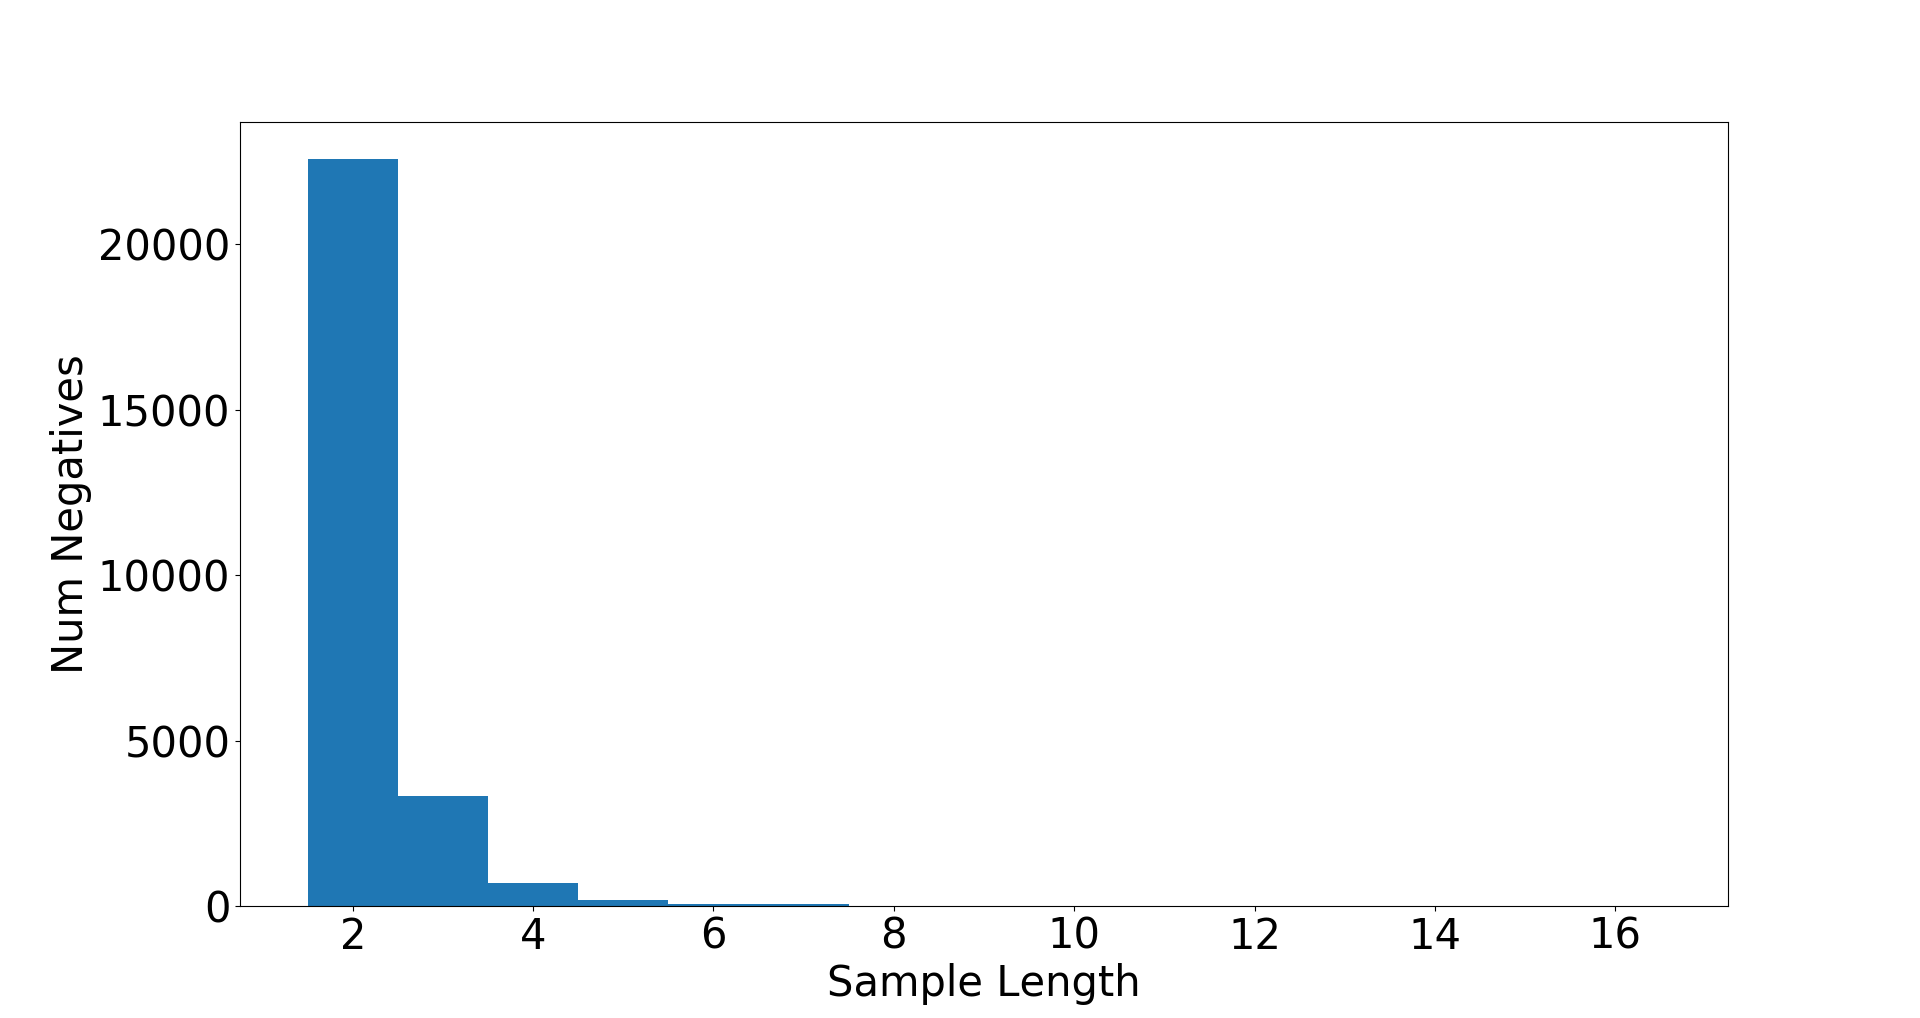
\includegraphics[width=.75\textwidth]{nSampleLenHistmin1_5max1_0Font.png}
  \caption{Distribution of pauses in the LRS3 dataset}
  \label{fig:negHist}
\end{figure}


As described earlier the LRS3 dataset is designed for visual speech recognition so it is important to analyze the dataset with respect to the usability for VVAD. Knowing the visual speech recognition background of the dataset it is quite obvious that the produced binary dataset will be very imbalanced. Figure \ref{fig:sampleDistribution} shows the theoretical distribution of positive and negative samples that can be created from the LRS3.
\begin{figure}
  \centering
  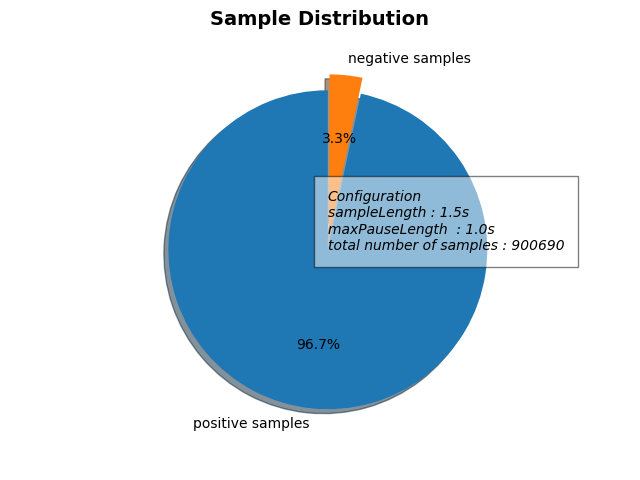
\includegraphics[width=.75\textwidth]{sampleDistribution.png}
  \caption{The theoretical distribution of positive and negative samples that can be created from the LRS3 with the given \texttt{sampleLength} and \texttt{maxPauseLength}}
  \label{fig:sampleDistribution}
\end{figure}
It shows that only 3.3\% fall in the negative class, while 96.7\% of the samples would be positive. Although that seems very little on the first look these 3.3\% are approximately 30 thousand samples, resulting in 12.5 hours of negative samples. 
For reasons of capacity it is decided to undersample the positive samples and take a positive-to-negative ratio of 1 to 1 (see section \ref{sec:problemsBigData}). 
This leads to over 60 thousand samples with an overall length of over 24 h.
In the process of creating those samples some appeared not to be valid, because the automatic conversion from the LRS3 samples to VVAD samples couldn't find a face or found to many in the corresponding LRS3 sample. 
This leads to 22,245 negative (\emph{not speaking}) samples and 22,244 positive (\emph{speaking}) samples and 18.5 h of learning data in total. 
The resulting samples are checked visually on a random basis to make sure the transformation from the LRS3 to the designated VVAD dataset is performed correctly.


With \texttt{sampleLength} and \texttt{maxPauseLength} set samples are extracted and the LRS3 dataset is transformed into a designated VVAD dataset.
At first the pauses, which later will be transformed to negative samples for the VVAD dataset, need to be extracted. 
Algorithm \ref{alg:detectPauses} shows how pauses are extracted from a LRS3 sample (an example of a LRS3 sample can be found in Appendix \ref{app:dataSample}).
Algorithm \ref{alg:detectPauses} is also used to analyze the LRS3 dataset and produce figure \ref{fig:negHist}.
From the these pauses negative and positive VVAD samples can be extracted.
Algorithm \ref{alg:getSampleConfigs} shows how the frames for the VVAD samples will be chosen from a LRS3 sample.
In section \ref{ssec:dataPreprocessing} is described how the preprocessing is performed and how the features for the VVAD sample will be extracted from a LRS3 video.

\begin{algorithm}[tbp]
\caption{}
\label{alg:detectPauses} 
\begin{algorithmic}[1]     % [1] = all lines are numbered
\Procedure{detectPauses}{$sample$}

	\Statex Returns a List of pauses in speech for a given LRS3 sample

	\algorithmicrequire{LRS3 Data Sample of speech}

	\algorithmicensure{List of Pauses}

	\State $oldWord \gets undefined$
	\State $listOfPauses \gets []$
	\State $maxPauseLength$ \Comment{defines the maximal length of a inter speech pause}

	\For{$word\ in\ sample$} \Comment{word consist of $start, end$ of the spoken word}

		\If{ $oldWord \ not \  undefined$}
		 \If{ $word.start - oldWord.end > maxPauseLength$}
				\State $listOfPauses.add((oldWord.end, word.start))$ \Comment{add pause to list}
		 \EndIf
 			\State $oldWord \gets word$

		\EndIf
		\EndFor
		
		\State \Return $listOfPauses$
\EndProcedure
\end{algorithmic}
\end{algorithm}

\begin{algorithm}[tbp]
\caption{}
\label{alg:getSampleConfigs} 
\begin{algorithmic}[1]     % [1] = all lines are numbered
\Procedure{getSampleConfigs}{$sample$}

	\Statex Returns a List of VVAD sample configs for a given LRS3 sample

	\algorithmicrequire{LRS3 Data Sample of speech}

	\algorithmicensure{List of VVAD sample configs}
	\State $sampleLength$ \Comment{defines the length of a VVAD sample}
	\State $k \gets sampleLength \times fps$ \Comment{defines the length the VVAD sample in frames}
		
	\State $listOfPauses \gets \textsc{detectPauses}(sample)$
	
	\State $negativeFrames \gets Set(listOfPauses)$ \Comment{set of frames corresponding to pauses}
	\State $sampleConfigs \gets []$
	\While{$frameNum\ in\ sample$}
		\State $nextFrames \gets Set(frameNum\ to\ frameNum + k)$
		\State $i \gets Intersection(negativeFrames, nextFrames)$ 
		\Switch{$i$}
    		\Case{$i == 0$} \Comment{It is a positive VVAD sample}
      			\State $sampleConfigs.add([True, nextFrames])$ \Comment{Add sample}
      			\State $frameNum += k$ \Comment{jump to the frame after the added sample}
    		\EndCase
		    \Case{$i == k$}\Comment{It is a negative VVAD sample}
      			\State $sampleConfigs.add([False, nextFrames])$ \Comment{Add sample}
      			\State $frameNum += k$ \Comment{jump to the frame after the added sample}
		    \EndCase
		    \Case{$0<i<k$}
		    	\State $frameNum += 1$ \Comment{just check the next k frames}
		    \EndCase
		\EndSwitch
	\EndWhile 
	
	\State \Return $sampleConfigs$

\EndProcedure
\end{algorithmic}
\end{algorithm}

\subsection{Data Preprocessing}\label{ssec:dataPreprocessing}
As described in section \ref{ssec:preprocessing} preprocessing is an elementary part of nearly every machine learning process. 
In the case of the VVAD the preprocessing handles the transformation from a video stream to VVAD samples consisting of \texttt{k} frames of features and a label. 
For every image in the stream a detected face will be followed throughout consecutive images in that stream. 
From these faces the VVAD sample will be extracted. 
The insights of how face detection and the tracking works can be found in Section \ref{ssec:faceDetection} and Section \ref{ssec:objectTracking}. 
For the End-to-End learning approach images are needed. 
These images need to be resized to a fixed size. 
To keep the original image ratio, zero padding needs to be applied in some cases.
Why a fixed image size is needed and the concept of zero padding is described in section \ref{ssec:reAndPad}.
For the facial features approach the features need to be normalized.
The preprocessing steps can also be used in live inference.


\subsubsection{Face Tracking}
To construct a VVAD sample from a LRS3 sample it is important to track a face in the video sequence, instead of only using face detection.
The approach of using only face detection can fail if multiple faces are present in the video.
To track a face dlib's correlation filter based tracker (see Section \ref{ssec:objectTracking}) is used.
On the tracked area a face detection (see Section \ref{ssec:faceDetection}) is performed to ensure correctness of the tracking and return an image of a face for every frame.
As described before the face tracking can also be used in a productive live system while making inference because inference needs to be done with samples of the same size as the training samples.


\subsubsection{Feature Generation}
To come from the tracked face to the features needed for the four different learning approaches described in Section \ref{ssec:algorithm} a \emph{Feature Generator} is implemented.
This feature generator takes a tracked image as input and outputs 
\begin{itemize}
\item[•] \textbf{Face Images -}  The whole image resized and zero padded to a specific size.
\item[•] \textbf{Lip Images -} An image of only the lips resized and zero padded to a specific size.
\item[•] \textbf{Face Features -} All 68 facial landmarks extracted with dlib's facial landmark detector
\item[•] \textbf{Lip Features -} All facial landmarks concerning the lips extracted with dlib's facial landmark detector 
\end{itemize}
For the face images the input image only needs to be resized and zero padded to a given size. Why and how this is done is described in Section \ref{ssec:reAndPad}.
For the other approaches dlib's facial landmark detector 
is used. 
As depicted in Figure \ref{fig:flavors} the predictor extracts the shape of a face given by 68 landmarks, whileas 20 of these landmarks are describing the lips.
The predictor is trained on the ibug 300-W face landmark dataset (\url{https://ibug.doc.ic.ac.uk/resources/facial-point-annotations/}). 
The iBUG 300-W face landmark dataset is provided for research purposes only. Commercial use (i.e., use in training commercial algorithms) is not allowed.
Because dlib's facial landmark detector is used to construct the VVAD dataset for lip images as well as the VVAD datasets for face and lip features, these fall under the same restrictions.
For the \emph{lip images} the minimal values in x- and y-direction are taken as the upper left corner of the lip image, while the lower right corner is defined by the maximal values in x- and y-direction.
The \emph{face features} are taken directly from the landmarks given from dlib's facial landmark detector. 
For the \emph{lip features} only landmark 49 to landmark 68 are taken into account, because they fully describe the lip shape as seen in Figure \ref{fig:shape}.
It is to mention that it is useful to normalize the features for \emph{face features} and \emph{lip features} when applied to a learning algorithm. 
The used normalization is described in Section \ref{ssec:normalize}.

\begin{figure}
  \centering
  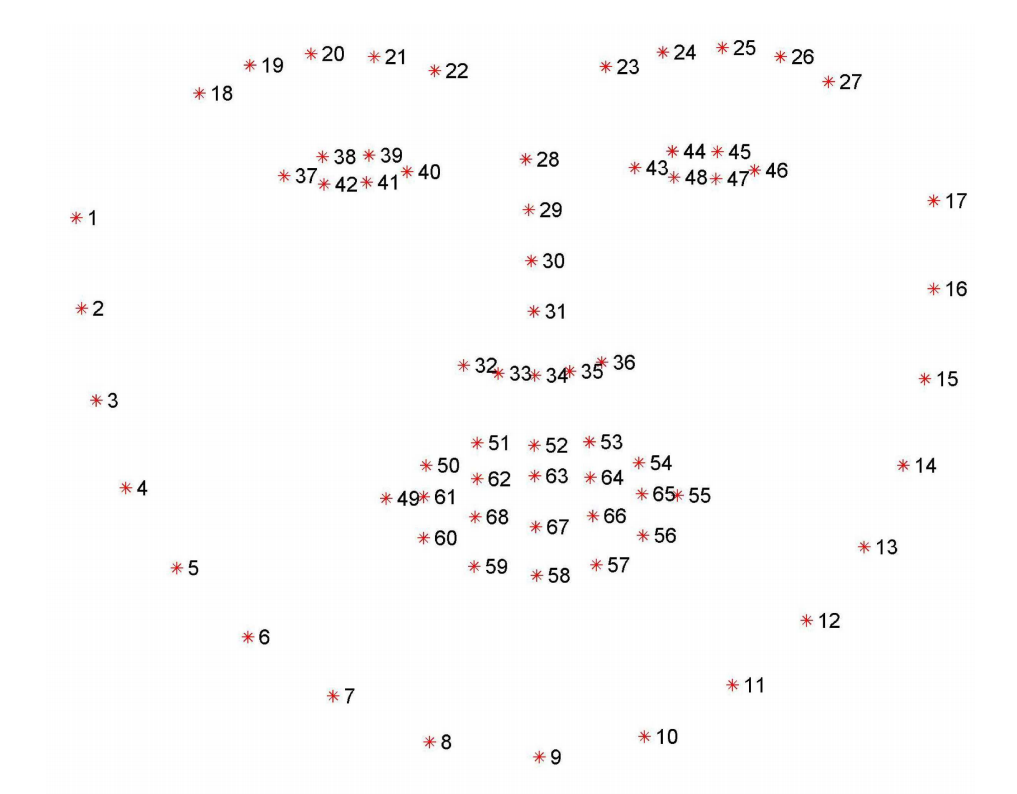
\includegraphics[width=.75\textwidth]{shape.png}
  \caption{The annotations given for the ibug 300-W dataset \cite{6755925}}
  \label{fig:shape}
\end{figure}

As well as the face tracking the generator can also be used in a live inference system to generate the features needed for the corresponding algorithm.


\subsubsection{Resize and Padding}\label{ssec:reAndPad}
Theoretically neural networks can work on images of different sizes, just like humans can detect a specific object even if they are only looking through a very small hole.
The limitations in artificial neural networks are computational.
Keras works with NumPy arrays as input. These are multidimensional arrays with fixed dimensions.
If gradient descent should be carried out with mini batches or the whole dataset the array will have a shape of $(DS \times SD)$ or $(BS \times SD)$ respectively, where $DS$ is the size of the whole dataset and $BS$ is the batch size, while $SD$ are the sample dimensions. The array for one batch of VVAD samples with the batch size 64 would have a shape of $(64 \times 38 \times 200 \times 200 \times 3)$ if face images would be considered and $(64 \times 38 \times 68)$ if face features would be considered.
The resizing is needed to produce a constant input size for the model but faces do not always have the same ratio and therefore the bounding boxes from the face detection do neither.
It is in fact important to keep the ratio of the face steady over all timesteps to reduce distortion over time which could be interpreted as mouth movement.
If a specific size is needed but it can't be fulfilled zero padding is a common technique to tackle this problem.
Zero padding just inputs zero values where no information can be provided. The NN will learn that zero means \emph{no information}.
For the resizing of face images this means that the face image is resized to the maximal size which would fit into the goal size and all pixels that can't be used on the right or lower site will be filled with zeros.




\subsection{Testing human Accuracy Level on the VVAD Dataset}\label{ssec:VVADHACL}
To test the VVAD dataset a human accuracy test was performed.
The test used a randomly seeded subset of 200 samples and was performed on 10 persons.
The overall human accuracy level was 87.93\% while the human accuracy level on positive samples is 91.44\% the human accuracy level on negative samples is only 84.44\%.
This shows, that the automatic extraction of the negative samples is more prone to errors than the automatic extraction of positive samples. This is due to the purpose of the LRS3 as a lipreading dataset which obviously offers more positive samples than negative samples for a VVAD dataset. 

\begin{figure}
  \centering
  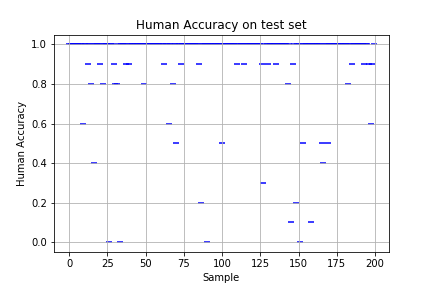
\includegraphics[width=.75\textwidth]{humanAcc.png}
  \caption{The human accuracy for each sample}
  \label{fig:humanAcc}
\end{figure}

\begin{figure}
  \centering
  \includegraphics[width=.75\textwidth]{PosHumanAcc.png}
  \caption{The human accuracy for each sample in the positive class}
  \label{fig:PosHumanAcc}
\end{figure}

\begin{figure}
  \centering
  \includegraphics[width=.75\textwidth]{NegHumanAcc.png}
  \caption{The human accuracy for each sample in the negative class}
  \label{fig:NegHumanAcc}
\end{figure}

In Figure \ref{fig:humanAcc} the accuracy for the individual samples is shown. Figure \ref{fig:PosHumanAcc} and \ref{fig:NegHumanAcc} show the human accuracy levels of each sample for the two classes.
It shows that a lot of the samples are classified with a very high accuracy, while some are obviously labeled wrong because they have a very high wrong classification rate. For the given reason these wrong labels appear more often in the negative class.
These wrongly labeled samples in the validation set make it hard to get a very high accuracy in the validation while tuning the learning algorithm.
But it is important to know this border, to tune to a value close to that.
If these wrongly labeled samples are not present in the test set, the accuracy of the final test can be higher. 
This shows how the learning algorithm can be robust against these outliers in the learning process. 

The test was implemented as a Web App using Node.js\cite{NODE} with Express\cite{EXPRESS} and a mongoDB\cite{MONGO} in the Back-End and HTML5 in the Front-End.
It shows a simple self explanatory graphical user interface which displays a video sequence of a \emph{speaking} or \emph{not speaking} person and three buttons (see figure \ref{fig:gui}). 
With the buttons it is possible to classify the sample as either \emph{speaking} or \emph{not speaking} and to repeat the video sequence.

\begin{figure}
  \centering
  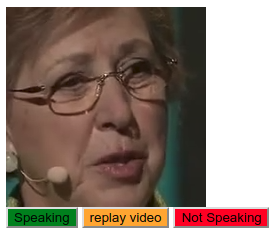
\includegraphics[width=.75\textwidth]{gui.png}
  \caption{The graphical user interface for the human accuracy test}
  \label{fig:gui}
\end{figure}



\section{Implementations of the Learning Algorithms}\label{sec:implLearning}
As stated in Section \ref{ssec:algorithm} LSTM-FCNs are state of the art in classification for video sequences and LSTMs in general work really well for time series.
To implement these Deep Learning techniques Keras is used.
Keras makes it possible to go very fast from a design to a prototype which makes it very valuable for research.
Following two End-to-End learning approaches and two approaches using manually extracted facial features will be presented.

End-to-End Learning describes a learning approach where raw data is feed to an ANN and the ANN is deep enough to learn all important features itself. For the example of a VVAD the ANN would be able to learn, that it makes sense to look for the mouth to see if a person is peaking or not.
In contrast in Section \ref{ssec:facialFeaturesLearninig} the important features are manually extracted before.
This approach needs more domain knowledge about the problem but can result in a substantially smaller model.
It is a common practice to start with the biggest possible model to get reasonable results to subsequently make the model small while trying to sustain accuracy.


\subsection{End-to-End Learning}\label{ssec:EndToEndLearning} %Maybe just one Chapter for End-to-End
To implement a End-to-End Learning Algorithm the following five Models  were taken to evaluate a Baseline:

\begin{itemize}
\item DenseNet201
\item DenseNet121
\item MobileNet
\item MobileNetV2
\item VGGFace
\end{itemize}

Where the first four Models are taken from the Keras Applications (\url{https://keras.io/applications/}), while the VGGFace is a taken from \url{https://github.com/rcmalli/keras-vggface}. 
DenseNet and MobileNet are more general models for image classification, that perform well on the ImageNet dataset \cite{imagenet_cvpr09}, whereas VGGFace was chosen because it is implemented explicitly for faces.
The Baseline Accuracy is taken from theses models applied on only the first image of every sample in the VVAD dataset.
Figure \ref{fig:baseAccDense201} to \ref{fig:baseAccVGGFace} show the accuracy for 200 epochs.
With this approach a Baseline Accuracy between 67.45\% for MobileNetV2 and 73.17\% for DenseNet121 can be reached.

\begin{figure}
  \centering
  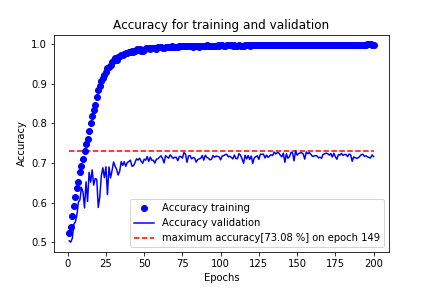
\includegraphics[width=.75\textwidth]{FINALBASELINEDenseNet_64_(96,96,3)_2019-08-0721:58:16029339_accuracy.png}
  \caption{Baseline Accuracy for DenseNet201}
  \label{fig:baseAccDense201}
\end{figure}

%\begin{figure}
%  \centering
%  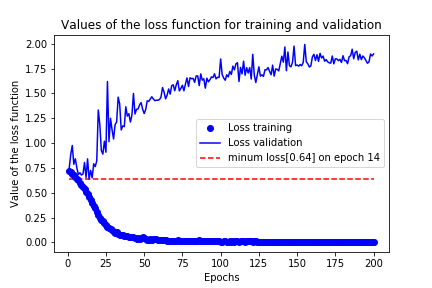
\includegraphics[width=.75\textwidth]{FINALBASELINEDenseNet_64_(96,96,3)_2019-08-0721:58:16029339_loss.png}
%  \caption{Baseline Loss for DenseNet201}
%  \label{fig:baseLossDense201}
%\end{figure}

%------------------------------

\begin{figure}
  \centering
  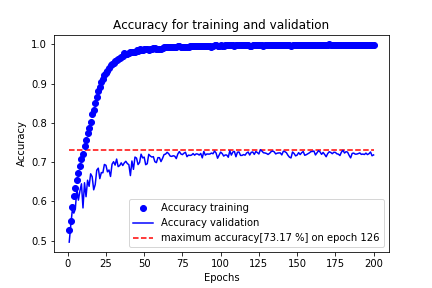
\includegraphics[width=.75\textwidth]{FINALBASELINEDenseNetSmall_64_(96,96,3)_2019-08-0817:39:46410269_accuracy.png}
  \caption{Baseline Accuracy for DenseNet121}
  \label{fig:baseAccDense121}
\end{figure}

%\begin{figure}
%  \centering
%  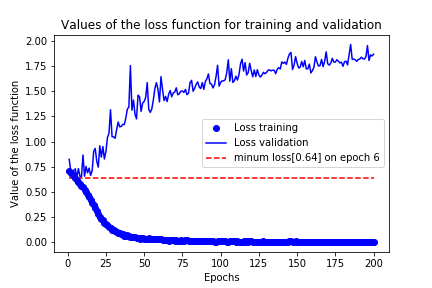
\includegraphics[width=.75\textwidth]{FINALBASELINEDenseNetSmall_64_(96,96,3)_2019-08-0817:39:46410269_loss.png}
%  \caption{Baseline Loss for DenseNet121}
%  \label{fig:baseLossDense121}
%\end{figure}

%%------------------------------

\begin{figure}
  \centering
  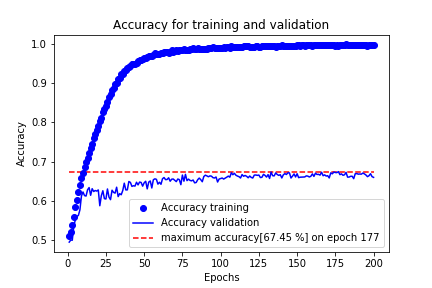
\includegraphics[width=.75\textwidth]{FINALBASELINEMobileNet_64_(96,96,3)_2019-08-0713:47:03006586_accuracy.png}
  \caption{Baseline Accuracy for MobileNetV2}
  \label{fig:baseAccMobile2}
\end{figure}

%\begin{figure}
%  \centering
%  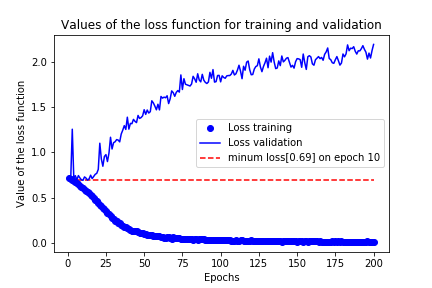
\includegraphics[width=.75\textwidth]{FINALBASELINEMobileNet_64_(96,96,3)_2019-08-0713:47:03006586_loss.png}
%  \caption{Baseline Loss for MobileNetV2}
%  \label{fig:baseLossMobile2}
%\end{figure}

%%------------------------------
%
\begin{figure}
  \centering
  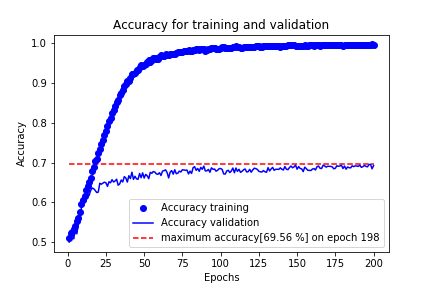
\includegraphics[width=.75\textwidth]{FINALBASELINEMobileNetV1_64_(96,96,3)_2019-08-0812:27:51418544_accuracy.png}
  \caption{Baseline Accuracy for MobileNetV1}
  \label{fig:baseAccMobile1}
\end{figure}

%\begin{figure}
%  \centering
%  \includegraphics[width=.75\textwidth]{FINALBASELINEMobileNetV1_64_(96,96,3)_2019-08-0812:27:51418544_loss.png}
%  \caption{Baseline Loss for MobileNetV1}
%  \label{fig:baseLossMobile1}
%\end{figure}
%
%%------------------------------

\begin{figure}
  \centering
  \includegraphics[width=.75\textwidth]{FINALBASELINEVGGFace_64_(96,96,3)_2019-08-0803:01:24022816_accuracy.png}
  \caption{Baseline Accuracy for VGGFace}
  \label{fig:baseAccVGGFace}
\end{figure}

%\begin{figure}
%  \centering
%  \includegraphics[width=.75\textwidth]{FINALBASELINEVGGFace_64_(96,96,3)_2019-08-0803:01:24022816_loss.png}
%  \caption{Baseline Loss for VGGFace}
%  \label{fig:baseLossVGGFace}
%\end{figure}

%------------------------------

The Baseline Models make spatial sense out of the images by producing meaningful features, which can be used to classify a single image.
This relies mostly on a combination of Convolutional Layers, as described in Section \ref{ssec:Conv}.
The optimal image size is evaluated for the MobileNet using quadratic image sizes starting from $32 \times 32$ to the maximal image size of $200 \time 200$ with a step size of 32.
Figure \ref{fig:AccOverImagesize} shows that the maximal accuracy in the spatial domain can be reached using a image size of $160 \times 160$.
\begin{figure}
  \centering
  \includegraphics[width=.75\textwidth]{AccOverImagesize.png}
  \caption{Evaluation of the optimal image size}
  \label{fig:AccOverImagesize}
\end{figure}


As described earlier speech can't be classified effectively by only one image, that's why the baseline accuracy levels around 70\% depending o the model.
To enhance these results a temporal sense must be extracted from a series of images.
To do so LSTM cells, as described in Section \ref{ssec:LSTM}, are used.
The overall model structure can be seen in Figure \ref{fig:model}.

\begin{figure}
  \centering
  \includegraphics[width=.75\textwidth]{modelStructure.png}
  \caption{Model structure using a \emph{TimeDistributed} Baseline Model}
  \label{fig:model}
\end{figure}

Here it can be seen, that a \emph{TimeDistributed} wrapper was used.
\emph{TimeDistributed} is a wrapper provided by Keras which basically copies a model for all timesteps, to effectively handle time series.
This allows the Baseline Models to be used to produce a time series from the features of all frames. 
The time series can be used by the LSTM Layer to make temporal sense, while the last Dense Layer is used to make the classification.
Experiments have shown that a single Dense layer with 512 units on top of a LSTM layer with 32 units show decent results.
To evaluate the increase in accuracy DenseNet121, MobileNet and VGGFace are used as base models in the \emph{TimeDistributed} wrapper and instead of only one image the first two images are taken in consideration.
Figure \ref{fig:tD2Dense} to \ref{fig:tD2VGGFace} show that DenseNet121, MobileNet and VGGFace improve by around 2.3\% with one more timestep.

\begin{figure}
  \centering
  \includegraphics[width=.75\textwidth]{all_TimeDistributedDenseNet_1_32_1_512_64_(2,96,96,3)_2019-08-1308:08:20668409_accuracy.png}
  \caption{Accuracy for a \emph{TimeDistributed} DenseNet121 on two timesteps}
  \label{fig:tD2Dense}
\end{figure}

\begin{figure}
  \centering
  \includegraphics[width=.75\textwidth]{all_TimeDistributedMobileNet_1_32_1_512_64_(2,96,96,3)_2019-08-1217:56:08538419_accuracy.png}
  \caption{Accuracy for a \emph{TimeDistributed} MobileNet on two timesteps}
  \label{fig:tD2Mobile}
\end{figure}

\begin{figure}
  \centering
  \includegraphics[width=.75\textwidth]{all_TimeDistributedVGGFace_1_32_1_512_64_(2,96,96,3)_2019-08-1316:53:40647699_accuracy.png}
  \caption{Accuracy for a \emph{TimeDistributed} VGGFace on two timesteps}
  \label{fig:tD2VGGFace}
\end{figure}

For more timesteps it can be seen in Figure \ref{fig:model} that the base model will be copied for every new timestep which results in a very fast growth of the model which can cause that the model is not trainable on modern Hardware.
To prevent that only the MobileNet as the smallest of the base models is taken further into consideration.
In comparison MobileNet trains approximately 4,2 million parameters while DenseNet trains around double the amount with 8 million parameters and VGGFace trains over 50 million parameters.
Knowing this the MobileNet is a good compromise between performance and size, because it is able to consider more timesteps, which in the end can lead to even higher accuracy.
The \emph{TimeDistributed} MobileNet with four timesteps already reaches a higher accuracy. Figure \ref{fig:AccTimeStepsMobile} shows how the accuracy raises over the number of used frames for the \emph{timeDistributred} MobileNet.

\begin{figure}
  \centering
  \includegraphics[width=.75\textwidth]{AccOverFrames.png}
  \caption{Validation Accuracy for the \emph{TimeDistributed} MobileNet over the number of timesteps/frames used.}
  \label{fig:AccTimeStepsMobile}
\end{figure}

Taking Figure \ref{fig:AccTimeStepsMobile} and \ref{fig:AccOverImagesize} into account the optimal values for the image size and number of frames are $160 \times 160$ and 36 respectively.
This model couldn't be trained on modern GPUs because it was to big for the internal memory. 
Since the image size has a quadratic influence on the memory consumption a image size of $96 \times 96$ was taken instead to make the training possible.
For the training of the model 15\% of the data is taken as validation data.
Figure \ref{fig:FaceEndToEndHistory} shows how the validation accuracy evolves over the training episodes.

\begin{figure}
  \centering
  \includegraphics[width=.75\textwidth]{FaceEndToEndHistory.png}
  \caption{The End-To-End Learning approach using Face Images reaches a Validation Accuracy of 94.05\%.}
  \label{fig:FaceEndToEndHistory}
\end{figure}

As described in Section \ref{ssec:VVADHACL} the overall human accuracy level is only 87.93\%.
The result of the End-To-End Learning approach on Face Images need to be evaluated on the test set, but the validation accuracy is a strong indicator that the produced model performs can reach \emph{superhuman performance}, which means it performs better than a human could do on the same task.

The same architecture is applied to the \emph{Lip Images} flavor of the VVAD dataset.
Here the domain knowledge about speech is applied as the assumption that the recognition of speech is only depending on the lips.
The results of the training are depicted in Figure \ref{fig:LipEndToEndHistory}.

\begin{figure}
  \centering
  \includegraphics[width=.75\textwidth]{LipEndToEndHistory.png}
  \caption{The End-To-End Learning approach using Lip Images reaches a Validation Accuracy of 93.98\%.}
  \label{fig:LipEndToEndHistory}
\end{figure}
As the validation accuracy went from 94.05\% for the Face Images only to 93.98\% for the Lip Images the assumption can be viewed as true. 
Taking only the Lip Images with the full resolution already reduces the amount of data needed to be kept in the GPU's RAM by approximately the half because the image size as the driving factor was reduced by half.
Also the trained model can be reduced in size from 35.6 MB to 29.3 MB.
These results need to be evaluated on the test set as well as the results of the approach using face images.

\subsection{Learning on Facial Features}\label{ssec:facialFeaturesLearninig} %Maybe just one Chapter for Facial Features
As described in Section \ref{sec:vvadData} the VVAD dataset also provides a version of the dataset which already exposes only facial landmarks.
In the End-To-End Learning approach features where produced from the images using MobileNet as a base model which was \emph{TimeDistributed} over k frames.
The resulting spatial features where forwarded to a LSTM layer to make temporal sense.
Since the \emph{face features} and \emph{lip features} flavor have already extracted spatial features it is no longer necessary to use a \emph{TimeDistributed} base model.
The facial landmarks are normalized as depicted in Section \ref{ssec:normalize} and then used by the head of the architecture used for the End-To-End Learning approach, which is a single LSTM layer with 32 units and a single Dense layer with 512 units.
Figure \ref{fig:FaceFeaturesHistory} shows that even with the substantially smaller dataset of the face features a validation accuracy of 89.79\% can be reached which is still higher than the human accuracy level.

\begin{figure}
  \centering
  \includegraphics[width=.75\textwidth]{FaceFeaturesHistory.png}
  \caption{The Facial Features for Learning approach using all 68 facial landmarks reaches a Validation Accuracy of 89.79\%.}
  \label{fig:FaceFeaturesHistory}
\end{figure}
The model size for this approach is approximately 100 times smaller with 342.5 KB.
But it is also visible that the validation accuracy is very unstable which is an indicator that it will not generalize as good as the prior models.
The essentially smaller model size can be a good compromise for weaker systems to perform the predictions to still get reasonable results.
An even smaller model can be trained with the lip features flavor of the VVAD dataset.
For this approach the same architecture as for the face features is used.
In Figure \ref{fig:LipFeaturesHistory} the validation accuracy over the epochs is displayed for the learning approach using only the 20 facial landmarks corresponding to the lips.

\begin{figure}
  \centering
  \includegraphics[width=.75\textwidth]{LipFeaturesHistory.png}
  \caption{The Facial Features for Learning approach using the 20 facial landmarks corresponding to the lips reaches a Validation Accuracy of 89.93\%.}
  \label{fig:LipFeaturesHistory}
\end{figure}

Here the accuracy is slightly better than the accuracy for using all 68 facial landmarks. 
This shows that the approach with all facial landmarks could probably be tuned a little more, but since the smaller model already shows higher accuracy it can be viewed as the tuned version of the approach using all facial landmarks.
Which also can be seen here is that the instability in the validation accuracy can be reduced.
This results need to be evaluated on the test set but the results for the validation accuracy are very promising that even for weaker hardware reliable predictions can be made.

\subsubsection{Feature Normalization}\label{ssec:normalize}
As described in Section \ref{ssec:normalization} normalizing features is a very helpful step to make NN more efficient.
Algorithm \ref{alg:normalize} describes how the facial landmarks extracted from dlib's facial landmark detector
are normalized.

\begin{algorithm}[tbp]
\caption{}
\label{alg:normalize} 
\begin{algorithmic}[1]     % [1] = all lines are numbered
\Procedure{calcDistances}{$sample$}

	\Statex Returns a List of euclidean distances to the first landmark in the sample
	
	\algorithmicrequire{List of facial landmarks }

	\algorithmicensure{List of euclidean distances}

	\State $base \gets sample[0][0]$
	\State $dists \gets []$
	\State $normalizedLandmarks \gets normalize(distances)$
	
	\For{$frame\ in\ sample$} 
		\State $distFrame \gets []$
		\For{$landmark\ in\ frame$} 
			\State $distPoint \gets []$
			\State $distPoint[0] = landmark[0] - base[0]$
			\State $distPoint[1] = landmark[1] - base[1]$
			\State $distFrame.append(distPoint)$
		\EndFor
		\State $dists.append(distFrame)$
	\EndFor
		\State \Return $dists$
\EndProcedure

\Procedure{normalize}{$distances$}

	\Statex Returns a List of normalized euclidean distances
	
	\algorithmicrequire{List of euclidean distances}

	\algorithmicensure{List of normalized euclidean distances}

	\State $absMax \gets max(abs(distances))$
	\State $normalizedDistances \gets []$
	\For{$frame\ in\ distances$} 
		\For{$dist in frame$}		
			\State $normalizedDist \gets dist / absMax$
			\State $normalizedDistances.append(normalizedDist)$
		\EndFor
	\EndFor
	
		\State \Return $normalizedDistances$
\EndProcedure

\Procedure{normalizeFacialLandmarks}{$landmarks$}

	\Statex Returns a List of normalized facial landmarks
	
	\algorithmicrequire{List of facial landmarks }

	\algorithmicensure{List of normalized facial landmarks}

	\State $distances \gets calcDistances(landmarks)$
	\State $normalizedLandmarks \gets normalize(distances)$
	
		\State \Return $normalizedLandmarks$
\EndProcedure
\end{algorithmic}
\end{algorithm}


%\chapter{Software}
\label{cha:software}
This chapter describes the software and libraries used to implement the VVAD.
In larger projects, independent if its software, hardware or even something else, it makes sense to
take advantage of the knowledge of others.
In terms of software this can be very easy, because the Internet is full of libraries, that provide solutions for various problems.
The few used to implement the VVAD are presented in the following.


%\chapter{Hardware}
\label{cha:hardware}
\section{Pepper}
\label{sec:pepper}
Pepper is a child sized humanoid social robot manufactured by SoftBank Robotics Group Corp.,
which can fulfill a wide range of purposes in different fields. Pepper is for example in
retail a lot to inform customers about special offers or articles in general. But it can also
be used as a receptionist in hotels or for entertainment in nursing homes.

\begin{figure}
\centering
\begin{subfigure}{.5\textwidth}
  \centering
  \includegraphics[width=\linewidth]{Pepper2.png}
  \caption{Measures without arms \cite{Pepper2018}}
\end{subfigure}%
\begin{subfigure}{.5\textwidth}
  \centering
  \includegraphics[width=\linewidth]{Pepper.png}
  \caption{Measures with arms \cite{Pepper2018}}
\end{subfigure}
\label{fig:pepper}
\end{figure}


It comes with the following sensors to perceive its surrounding:
\subsection*{Sensors}
\begin{description}
  \item [Inertial unit] Pepper is equipped with an Inertial unit, made of:
    \begin{itemize}
      \item a 3-axis gyroscope with an angular speed of ~500 °/s,
      \item a 3-axis accelerometer with an acceleration of ~2 g.
    \end{itemize}
  \item [Lasers] Pepper is equipped with 6 laser sensors which lets him evaluate its surrounding and the ground in front of it.
  \item [Infra-Red] Pepper is equipped with 2 infra-red sensors for obstacle detection
  \item [Sonars] Pepper is equipped with two ultrasonic sensors (or sonars) which allow it to estimate the distance to obstacles in its environment.
  \item [MRE] Peppers servo motors use MRE (Magnetic Rotary Encoders) using Hall-effect sensor technology.
  \item [Contact and tactile sensors] Pepper is equipped with different buttons and tactile sensors:
    \begin{itemize}
      \item Power button
      \item Emergency switch
      \item 3 tactile sensors on the head
      \item One tactile sensor on the back of every hand
      \item 3 bumpers on the base
    \end{itemize}
  \item [Video \& depth sensors] Pepper is equipped with a depth camera in the eyes and one camera in the mouth and another one in its head.
  \item [Microphones] Pepper is equipped with 4 microphones on its head to allow echo location
\end{description}

\begin{figure}
  \centering
  \includegraphics[width=.75\textwidth]{PepperOverview.jpg}
  \caption{Overview for Peppers sensors and actuators. \cite{pepperOverview}}
  \label{fig:pepperOverview}
\end{figure}

\subsection*{Actuators}
To act on the data acquired through the sensors Pepper has the following actuators:
\begin{description}
  \item [Loudspeakers] To speak very naturally to humans Pepper has two loudspeakers in its ears
  \item [LEDs] To indicate different signals Pepper uses LEDs in its shoulder, ears and eyes.
  \item [Motors] Pepper is equipped with a bunch of motors to move itself and different parts of its body:
  \begin{description}
    \item [Head] Pepper has motors for head yaw	and head pitch to move the field of view.
    \item [Arms] Pepper has motors for shoulder pitch, shoulder roll, elbow yaw and elbow roll to move the arms for gestures
    \item [Hands] Pepper has motors for wrist yaw	and grasping for gestures
    \item [Legs] Pepper has motors hip roll, hip pitch and knee pitch for leaning for- and backward.
    \item [Base] Pepper has motors for the 3 omnidirectional wheels on the base to drive around.
  \end{description}
\end{description}

\subsection*{Tablet}
Besides all the listed sensors and actuators Pepper is also equipped with a tablet, which gives the robot another feature for communication with humans. The tablet can be seen as an extra hybrid sensing and acting system, because it has sensing capabilities with the built-in camera and the touchscreen, but it also provides an actuator with the screen.

\subsection*{Internals}
To complete the robotic system a central processing unit and power supply is needed.
Pepper therefore is equipped with a Atom E3845 Quad core and 4 GB DDR3 RAM as well as a Lithium-ion battery with a capacity of 30 Ah, which lets Pepper operate for a whole workday without the need to recharge.
To communicate with other electronic devices Pepper is also equipped with a WiFi-chip which provides the IEEE 802.11 a/b/g/n standard and a Bluetooth-chip of Version 4.0.

To see the detailed description and illustrations of Pepper we forward the interested reader to \cite{Pepper2018}


\chapter{Experimental Evaluation}
\label{cha:eval}
As described in Section \ref{ssec:dataTheory} the models are trained on a designated training set while tuning the model is performed on the validation set.
To really evaluate how the models perform on totally new data a test set is hold back and is only used to evaluate the produced model once in the very end.
This so-called \emph{holdback method} is used to evaluate the models produced in Section \ref{sec:implLearning}.
For this matter the model will predict every sample from the test set and the prediction is compared with the original label of the sample.
With this the accuracy can be calculated as
\begin{equation}
Accuracy = \frac{TP + TN}{TP + TN + FP + FN}
\end{equation}
where $TP$, $TN$, $FP$ and $FN$ are the numbers of true positive, true negative, false positive and false negative classifications respectively.
Furthermore the Mean Absolute Error (MAE) can give a clue about how certain the model was making this classifications.
The MAE is calculated by 
\begin{equation}
\frac{1}{n} \sum_{i=1}^n |\hat{Y}_i - Y_i|
\end{equation}
where $n$ is the number of classifications, $\hat{Y}_i$ is the classification given by the model and $Y_i$ the label.
Additionally to that 4 of the wrong labeled samples (see Section \ref{ssec:VVADHACL}) will be taken into deeper investigation.
It is interesting to see here how the models act on that samples. 

\section{Wrong labeled samples in the test set}\label{sec:wrongLabels}
In the human accuracy test some of the samples were labeled wrong or at least were classified with the opposite class label.
A closer look is taken into four of these samples from the test set.
While the samples \texttt{31366} and \texttt{42768} are labeled positive from the automatic transformation from the LRS3 sample to the VVAD sample they were classified as negative by all the subjects in the human accuracy level test.
For the samples \texttt{14679} and \texttt{6178} the opposite is the case.
On further investigation it was seen that sample \texttt{14679} and \texttt{42768} are obviously wrong labeled while sample \texttt{31366} and \texttt{6178} have some special properties that make them perform very bad on the human accuracy level test.
Sample \texttt{31366} has a very quick head movement which makes it very hard to see the very little movements of the mouth to produce speech.
Sample \texttt{6178} shows a person obviously producing sound with his mouth.
But the sound here is no speech but \emph{beat boxing} which is not considered speech in the original LRS3 dataset.
Sample \texttt{6178} and \texttt{31366} are depicted in Figure \ref{fig:6178} and \ref{fig:31366} respectively.

\begin{figure}
\centering
\parbox{\textwidth}{
\begin{subfigure}{0.09\textwidth}
  \centering
  \includegraphics[width=\linewidth]{6178_faceImage_0/cropped_img-0.png}
\end{subfigure}
\begin{subfigure}{0.09\textwidth}
  \centering
  \includegraphics[width=\linewidth]{6178_faceImage_0/cropped_img-1.png}
\end{subfigure}
\begin{subfigure}{0.09\textwidth}
  \centering
  \includegraphics[width=\linewidth]{6178_faceImage_0/cropped_img-2.png}
\end{subfigure}
\begin{subfigure}{0.09\textwidth}
  \centering
  \includegraphics[width=\linewidth]{6178_faceImage_0/cropped_img-3.png}
\end{subfigure}
\begin{subfigure}{0.09\textwidth}
  \centering
  \includegraphics[width=\linewidth]{6178_faceImage_0/cropped_img-4.png}
\end{subfigure}
\begin{subfigure}{0.09\textwidth}
  \centering
  \includegraphics[width=\linewidth]{6178_faceImage_0/cropped_img-5.png}
\end{subfigure}
\begin{subfigure}{0.09\textwidth}
  \centering
  \includegraphics[width=\linewidth]{6178_faceImage_0/cropped_img-6.png}
\end{subfigure}
\begin{subfigure}{0.09\textwidth}
  \centering
  \includegraphics[width=\linewidth]{6178_faceImage_0/cropped_img-7.png}
\end{subfigure}
\begin{subfigure}{0.09\textwidth}
  \centering
  \includegraphics[width=\linewidth]{6178_faceImage_0/cropped_img-8.png}
\end{subfigure}
\begin{subfigure}{0.09\textwidth}
  \centering
  \includegraphics[width=\linewidth]{6178_faceImage_0/cropped_img-9.png}
\end{subfigure}
}
\parbox{\textwidth}{
\begin{subfigure}{0.09\textwidth}
  \centering
  \includegraphics[width=\linewidth]{6178_faceImage_0/cropped_img-10.png}
\end{subfigure}
\begin{subfigure}{0.09\textwidth}
  \centering
  \includegraphics[width=\linewidth]{6178_faceImage_0/cropped_img-11.png}
\end{subfigure}
\begin{subfigure}{0.09\textwidth}
  \centering
  \includegraphics[width=\linewidth]{6178_faceImage_0/cropped_img-12.png}
\end{subfigure}
\begin{subfigure}{0.09\textwidth}
  \centering
  \includegraphics[width=\linewidth]{6178_faceImage_0/cropped_img-13.png}
\end{subfigure}
\begin{subfigure}{0.09\textwidth}
  \centering
  \includegraphics[width=\linewidth]{6178_faceImage_0/cropped_img-14.png}
\end{subfigure}
\begin{subfigure}{0.09\textwidth}
  \centering
  \includegraphics[width=\linewidth]{6178_faceImage_0/cropped_img-15.png}
\end{subfigure}
\begin{subfigure}{0.09\textwidth}
  \centering
  \includegraphics[width=\linewidth]{6178_faceImage_0/cropped_img-16.png}
\end{subfigure}
\begin{subfigure}{0.09\textwidth}
  \centering
  \includegraphics[width=\linewidth]{6178_faceImage_0/cropped_img-17.png}
\end{subfigure}
\begin{subfigure}{0.09\textwidth}
  \centering
  \includegraphics[width=\linewidth]{6178_faceImage_0/cropped_img-18.png}
\end{subfigure}
\begin{subfigure}{0.09\textwidth}
  \centering
  \includegraphics[width=\linewidth]{6178_faceImage_0/cropped_img-19.png}
\end{subfigure}
}
\parbox{\textwidth}{
\begin{subfigure}{0.09\textwidth}
  \centering
  \includegraphics[width=\linewidth]{6178_faceImage_0/cropped_img-20.png}
\end{subfigure}
\begin{subfigure}{0.09\textwidth}
  \centering
  \includegraphics[width=\linewidth]{6178_faceImage_0/cropped_img-21.png}
\end{subfigure}
\begin{subfigure}{0.09\textwidth}
  \centering
  \includegraphics[width=\linewidth]{6178_faceImage_0/cropped_img-22.png}
\end{subfigure}
\begin{subfigure}{0.09\textwidth}
  \centering
  \includegraphics[width=\linewidth]{6178_faceImage_0/cropped_img-23.png}
\end{subfigure}
\begin{subfigure}{0.09\textwidth}
  \centering
  \includegraphics[width=\linewidth]{6178_faceImage_0/cropped_img-24.png}
\end{subfigure}
\begin{subfigure}{0.09\textwidth}
  \centering
  \includegraphics[width=\linewidth]{6178_faceImage_0/cropped_img-25.png}
\end{subfigure}
\begin{subfigure}{0.09\textwidth}
  \centering
  \includegraphics[width=\linewidth]{6178_faceImage_0/cropped_img-26.png}
\end{subfigure}
\begin{subfigure}{0.09\textwidth}
  \centering
  \includegraphics[width=\linewidth]{6178_faceImage_0/cropped_img-27.png}
\end{subfigure}
\begin{subfigure}{0.09\textwidth}
  \centering
  \includegraphics[width=\linewidth]{6178_faceImage_0/cropped_img-28.png}
\end{subfigure}
\begin{subfigure}{0.09\textwidth}
  \centering
  \includegraphics[width=\linewidth]{6178_faceImage_0/cropped_img-29.png}
\end{subfigure}
}
\parbox{\textwidth}{
\begin{subfigure}{0.09\textwidth}
  \centering
  \includegraphics[width=\linewidth]{6178_faceImage_0/cropped_img-30.png}
\end{subfigure}
\begin{subfigure}{0.09\textwidth}
  \centering
  \includegraphics[width=\linewidth]{6178_faceImage_0/cropped_img-31.png}
\end{subfigure}
\begin{subfigure}{0.09\textwidth}
  \centering
  \includegraphics[width=\linewidth]{6178_faceImage_0/cropped_img-32.png}
\end{subfigure}
\begin{subfigure}{0.09\textwidth}
  \centering
  \includegraphics[width=\linewidth]{6178_faceImage_0/cropped_img-33.png}
\end{subfigure}
\begin{subfigure}{0.09\textwidth}
  \centering
  \includegraphics[width=\linewidth]{6178_faceImage_0/cropped_img-34.png}
\end{subfigure}
\begin{subfigure}{0.09\textwidth}
  \centering
  \includegraphics[width=\linewidth]{6178_faceImage_0/cropped_img-35.png}
\end{subfigure}
\begin{subfigure}{0.09\textwidth}
  \centering
  \includegraphics[width=\linewidth]{6178_faceImage_0/cropped_img-36.png}
\end{subfigure}
\begin{subfigure}{0.09\textwidth}
  \centering
  \includegraphics[width=\linewidth]{6178_faceImage_0/cropped_img-37.png}
\end{subfigure}
}
\caption{Sample \texttt{6178} is labeled as a negative (\emph{not speaking}) sample by the automatic transformation from LRS3 to VVAD dataset. On the human accuracy level test 100\% of the subjects classified the sample as positive (\emph{speaking}) sample. Beat boxing is not considered speech in the LRS3 dataset, which causes the wrong label.}
\label{fig:6178}
\end{figure}


\begin{figure}
\centering
\parbox{\textwidth}{
\begin{subfigure}{0.09\textwidth}
  \centering
  \includegraphics[width=\linewidth]{31366_faceImage_1/cropped_img-0.png}
\end{subfigure}
\begin{subfigure}{0.09\textwidth}
  \centering
  \includegraphics[width=\linewidth]{31366_faceImage_1/cropped_img-1.png}
\end{subfigure}
\begin{subfigure}{0.09\textwidth}
  \centering
  \includegraphics[width=\linewidth]{31366_faceImage_1/cropped_img-2.png}
\end{subfigure}
\begin{subfigure}{0.09\textwidth}
  \centering
  \includegraphics[width=\linewidth]{31366_faceImage_1/cropped_img-3.png}
\end{subfigure}
\begin{subfigure}{0.09\textwidth}
  \centering
  \includegraphics[width=\linewidth]{31366_faceImage_1/cropped_img-4.png}
\end{subfigure}
\begin{subfigure}{0.09\textwidth}
  \centering
  \includegraphics[width=\linewidth]{31366_faceImage_1/cropped_img-5.png}
\end{subfigure}
\begin{subfigure}{0.09\textwidth}
  \centering
  \includegraphics[width=\linewidth]{31366_faceImage_1/cropped_img-6.png}
\end{subfigure}
\begin{subfigure}{0.09\textwidth}
  \centering
  \includegraphics[width=\linewidth]{31366_faceImage_1/cropped_img-7.png}
\end{subfigure}
\begin{subfigure}{0.09\textwidth}
  \centering
  \includegraphics[width=\linewidth]{31366_faceImage_1/cropped_img-8.png}
\end{subfigure}
\begin{subfigure}{0.09\textwidth}
  \centering
  \includegraphics[width=\linewidth]{31366_faceImage_1/cropped_img-9.png}
\end{subfigure}
}
\parbox{\textwidth}{
\begin{subfigure}{0.09\textwidth}
  \centering
  \includegraphics[width=\linewidth]{31366_faceImage_1/cropped_img-10.png}
\end{subfigure}
\begin{subfigure}{0.09\textwidth}
  \centering
  \includegraphics[width=\linewidth]{31366_faceImage_1/cropped_img-11.png}
\end{subfigure}
\begin{subfigure}{0.09\textwidth}
  \centering
  \includegraphics[width=\linewidth]{31366_faceImage_1/cropped_img-12.png}
\end{subfigure}
\begin{subfigure}{0.09\textwidth}
  \centering
  \includegraphics[width=\linewidth]{31366_faceImage_1/cropped_img-13.png}
\end{subfigure}
\begin{subfigure}{0.09\textwidth}
  \centering
  \includegraphics[width=\linewidth]{31366_faceImage_1/cropped_img-14.png}
\end{subfigure}
\begin{subfigure}{0.09\textwidth}
  \centering
  \includegraphics[width=\linewidth]{31366_faceImage_1/cropped_img-15.png}
\end{subfigure}
\begin{subfigure}{0.09\textwidth}
  \centering
  \includegraphics[width=\linewidth]{31366_faceImage_1/cropped_img-16.png}
\end{subfigure}
\begin{subfigure}{0.09\textwidth}
  \centering
  \includegraphics[width=\linewidth]{31366_faceImage_1/cropped_img-17.png}
\end{subfigure}
\begin{subfigure}{0.09\textwidth}
  \centering
  \includegraphics[width=\linewidth]{31366_faceImage_1/cropped_img-18.png}
\end{subfigure}
\begin{subfigure}{0.09\textwidth}
  \centering
  \includegraphics[width=\linewidth]{31366_faceImage_1/cropped_img-19.png}
\end{subfigure}
}
\parbox{\textwidth}{
\begin{subfigure}{0.09\textwidth}
  \centering
  \includegraphics[width=\linewidth]{31366_faceImage_1/cropped_img-20.png}
\end{subfigure}
\begin{subfigure}{0.09\textwidth}
  \centering
  \includegraphics[width=\linewidth]{31366_faceImage_1/cropped_img-21.png}
\end{subfigure}
\begin{subfigure}{0.09\textwidth}
  \centering
  \includegraphics[width=\linewidth]{31366_faceImage_1/cropped_img-22.png}
\end{subfigure}
\begin{subfigure}{0.09\textwidth}
  \centering
  \includegraphics[width=\linewidth]{31366_faceImage_1/cropped_img-23.png}
\end{subfigure}
\begin{subfigure}{0.09\textwidth}
  \centering
  \includegraphics[width=\linewidth]{31366_faceImage_1/cropped_img-24.png}
\end{subfigure}
\begin{subfigure}{0.09\textwidth}
  \centering
  \includegraphics[width=\linewidth]{31366_faceImage_1/cropped_img-25.png}
\end{subfigure}
\begin{subfigure}{0.09\textwidth}
  \centering
  \includegraphics[width=\linewidth]{31366_faceImage_1/cropped_img-26.png}
\end{subfigure}
\begin{subfigure}{0.09\textwidth}
  \centering
  \includegraphics[width=\linewidth]{31366_faceImage_1/cropped_img-27.png}
\end{subfigure}
\begin{subfigure}{0.09\textwidth}
  \centering
  \includegraphics[width=\linewidth]{31366_faceImage_1/cropped_img-28.png}
\end{subfigure}
\begin{subfigure}{0.09\textwidth}
  \centering
  \includegraphics[width=\linewidth]{31366_faceImage_1/cropped_img-29.png}
\end{subfigure}
}
\parbox{\textwidth}{
\begin{subfigure}{0.09\textwidth}
  \centering
  \includegraphics[width=\linewidth]{31366_faceImage_1/cropped_img-30.png}
\end{subfigure}
\begin{subfigure}{0.09\textwidth}
  \centering
  \includegraphics[width=\linewidth]{31366_faceImage_1/cropped_img-31.png}
\end{subfigure}
\begin{subfigure}{0.09\textwidth}
  \centering
  \includegraphics[width=\linewidth]{31366_faceImage_1/cropped_img-32.png}
\end{subfigure}
\begin{subfigure}{0.09\textwidth}
  \centering
  \includegraphics[width=\linewidth]{31366_faceImage_1/cropped_img-33.png}
\end{subfigure}
\begin{subfigure}{0.09\textwidth}
  \centering
  \includegraphics[width=\linewidth]{31366_faceImage_1/cropped_img-34.png}
\end{subfigure}
\begin{subfigure}{0.09\textwidth}
  \centering
  \includegraphics[width=\linewidth]{31366_faceImage_1/cropped_img-35.png}
\end{subfigure}
\begin{subfigure}{0.09\textwidth}
  \centering
  \includegraphics[width=\linewidth]{31366_faceImage_1/cropped_img-36.png}
\end{subfigure}
\begin{subfigure}{0.09\textwidth}
  \centering
  \includegraphics[width=\linewidth]{31366_faceImage_1/cropped_img-37.png}
\end{subfigure}
}
\caption{Sample \texttt{31366} is labeled as a positive (\emph{speaking}) sample by the automatic transformation from LRS3 to VVAD dataset. On the human accuracy level test 100\% of the subjects classified the sample as negative (\emph{not speaking}) sample. The fast movement of the head while producing only a small movement of the lips causes the wrong label.}
\label{fig:31366}
\end{figure}

\section{End-to-End Learning}
As described in Section \ref{ssec:EndToEndLearning} the models trained on images of faces or lips perform quite well on the validation set.
Here accuracies over 90\% could be reached.
The test described earlier reaches a \emph{test accuracy} of 92\% 
for the model trained on faces.
This model has a MAE of $0.08$. 
The classifications of this can be seen in Figure \ref{fig:testFaceImages}.
The first 100 samples are negative samples while the last 100 samples are positive samples and the arrows show the probability, given by the model, that this sample belongs to the positive class.
The red dashed line is the decision boundary on which the model decides its classifications. 
This visualizeses how certain the model is with its predictions.

The smaller model which was only trained on images of the lips reaches a \emph{test accuracy} of 92\% with a MAE of $0.09$.
The classifications on the test set made by this model are depicted in Figure \ref{fig:testLipImages}.
Similar to the performances in the validation set the performances in the test set are very close to each other.
The bigger model adds only a very small improvement to the \emph{test accuracy}

\begin{figure}
  \centering
  \includegraphics[width=.75\textwidth]{testFaceImages.png}
  \caption{Visualization of the classifications on the test set for the model which was trained on images of faces.}
  \label{fig:testFaceImages}
\end{figure}

\begin{figure}
  \centering
  \includegraphics[width=.75\textwidth]{testLipImages.png}
  \caption{Visualization of the classifications on the test set for the model which was trained on images of lips.}
  \label{fig:testLipImages}
\end{figure}

The performance on the wrong labeled samples described in Section \ref{sec:wrongLabels} is shown in Figure \ref{fig:testWrongFaceImages} - \ref{fig:testWrongLipImages}.
Here it can be seen that the model performs exactly the same as the human subjects in the human accuracy level test.

\begin{figure}
  \centering
  \includegraphics[width=.75\textwidth]{testWrongFaceImages.png}
  \caption{Visualization of the classifications on wrong labeled samples in the test set for the model which was trained on images of faces.}
  \label{fig:testWrongFaceImages}
\end{figure}

\begin{figure}
  \centering
  \includegraphics[width=.75\textwidth]{testWrongLipImages.png}
  \caption{Visualization of the classifications on wrong labeled samples in the test set for the model which was trained on images of lips.}
  \label{fig:testWrongLipImages}
\end{figure}


\section{Learning on Facial Features}
As described in Section \ref{ssec:facialFeaturesLearninig} the models trained on the facial landmarks perform quite well on the validation set.
For the model trained on all 68 facial landmarks the conducted test delivered a \emph{test accuracy} of 89\%
and a MAE of $0.15$. 
This shows that the model also generalizes very well on data it was never in contact with.
Figure \ref{fig:testFaceFeatures} shows the classifications made by the model.


\begin{figure}
  \centering
  \includegraphics[width=.75\textwidth]{testFaceFeatures.png}
  \caption{Visualization of the classifications on the test set for the model which uses all 68 facial landmarks.}
  \label{fig:testFaceFeatures}
\end{figure}

\begin{figure}
  \centering
  \includegraphics[width=.75\textwidth]{testLipFeatures.png}
  \caption{Visualization of the classifications on the test set for the model which uses the 20 facial landmarks corresponding to the lips.}
  \label{fig:testLipFeatures}
\end{figure}

While in the validation set the model trained on the 20 facial landmarks corresponding to the lips performed nearly the same this behavior hold in the test set.
Figure \ref{fig:testLipFeatures} shows the classifications made by the model.
The model reaches a \emph{test accuracy} of 89\% with a MAE of $0.16$.
This shows that the models are performing nearly the same although the model trained on the face features is 1.4 times bigger than the model trained on the lip features.
Although the models trained on the facial features perform nearly as good as the ones using the End-To-End Learning approach Figure \ref{fig:testFaceImages} - \ref{fig:testLipFeatures} visualize very well the fact that the End-To-End models have less uncertainty in their predictions.

The performance on the wrong labeled samples for the models trained on facial features are depicted in Figure \ref{fig:testWrongFaceFeatures} - \ref{fig:testWrongLipFeatures}.
These results show that the model trained only on the facial landmarks of the lips was able to correctly classify sample \texttt{31366} although humans were not able to do so. 
Also sample \texttt{6178} shows a prediction closer to the decision boundary which means the model has a higher uncertainty on this classification.

\begin{figure}
  \centering
  \includegraphics[width=.75\textwidth]{testWrongFaceFeatures.png}
  \caption{Visualization of the classifications on wrong labeled samples in the test set for the model which uses all 68 facial landmarks.}
  \label{fig:testWrongFaceFeatures}
\end{figure}

\begin{figure}
  \centering
  \includegraphics[width=.75\textwidth]{testWrongLipFeatures.png}
  \caption{Visualization of the classifications on wrong labeled samples in the test set for the model which uses the 20 facial landmarks corresponding to the lips.}
  \label{fig:testWrongLipFeatures}
\end{figure}


\section{Interpretation}\label{sec:interpretation}
All described models reach a \emph{superhuman performance} not only while validation but also in the test set.
Table \ref{tb:accuracies} shows an overview of the accuracies reached by the different approaches.

\begin{table}[h!]
\centering
\begin{tabular}{|l|c|c|}
\hline
\textbf{Model} & \textbf{Accuracy} & \textbf{MAE} \\
\hline
Face Images & 92\% & 0.08 \\
\hline
Lip Images & 92\% & 0.09 \\
\hline
Face Features &  89\% & 0.15 \\
\hline
Lip Features & 89\% & 0.16 \\
\hline
\end{tabular}
\caption{Overview of the performance of the different models}
\label{tb:accuracies}
\end{table}

This shows that the cognitive skill can be used very reliable to improve various applications in the field of social robotics to make Human-Machine-Interaction more natural.
Additionally it was shown that the assumption that VVAD mostly depends on the lips holds true.
This helps to understand VVAD in more depth and makes it possible to generate smaller models while sustaining high accuracy.
Furthermore it was shown that \emph{Deep Learning} is a very generic approach that can reach very high accuracy but on the downside produces very big models and modern GPUs might reach their limits training such models.
In this aspect, research is required to design techniques that use regularization during training time to allow the model to shrink during training.
Until more robust and clever regularization mechanism are found \emph{feature engineering} is still a valuable task in the world of machine learning to reduce model size and training time.
This is highlighted by the results of the models trained on the facial landmarks that reach nearly as high accuracy as the End-To-End approaches but consume only a fraction of the memory and also the training time could be reduced massively.
Besides that feature engineering brings the advantage that the human designer of the learning algorithm can very precisely define what features will be used to learn which gives more comprehensibility to the designed algorithm.
But it also limits the model to the assumptions made by the human designer.
This can be shown in the comparison of the End-To-End approach and the feature engineered approach using the facial landmarks.
The latter shows more instability in the learning as seen in Figure \ref{fig:FaceFeaturesHistory} and a higher uncertainty in the predictions shown in Figure \ref{fig:testFaceFeatures} and a higher MAE for this approach.


%\chapter{Figures, Tables, Source Code}
\label{cha:Figures}

%\chapter[Mathematical Elements]{Mathematical Elements, Equations and Algorithms}
\label{cha:Mathematics}


%\chapter[Umgang mit Literatur]{Umgang mit Literatur und anderen Quellen}
\label{cha:Literatur}

\paragraph{Anmerkung:}
Der Titel dieses Kapitels ist absichtlich so
lang geraten, dass er nicht mehr in die Kopfzeile der Seiten passt.
In diesem Fall kann in der \verb!\chapter!-Anweisung
als optionales Argument \verb![..]! ein verkürzter Text für die
Kopfzeile (und das Inhaltsverzeichnis) angegeben werden:
%
\begin{LaTeXCode}[numbers=none]
\chapter[Umgang mit Literatur]{Umgang mit Literatur und anderen Quellen}
\end{LaTeXCode}

\section{Allgemeines}

Der richtige Umgang mit Quellen ist ein wesentliches Element bei der Erstellung
wissenschaftlicher Arbeiten im Allgemeinen (\sa\ Abschnitt \ref{sec:Plagiarismus}).
Für die Gestaltung von Quellenangaben sind unterschiedlichste Richtlinien in
Gebrauch, bestimmt \ua\ vom jeweiligen Fachgebiet oder Richtlinien von Verlagen und Hochschulen.
Diese Vorlage sieht ein Schema vor, das in den natur\-wissen\-schaftlich-technischen
Disziplinen üblich ist.%
\footnote{Anpassungen an andere Formen sind relativ leicht möglich.}
Technisch basiert dieser Teil auf \texttt{BibTeX} \cite{Patashnik1988}
\bzw\ \texttt{Biber}%
\footnote{Wird seit Version 2013/02/19 anstelle von \texttt{bibtex} verwendet
	(s.\ \url{http://biblatex-biber.sourceforge.net/}),}
in Kombination mit dem Paket \texttt{biblatex} \cite{Lehman2016}.


Die Verwaltung von Quellen besteht grundsätzlich aus zwei Elementen:
\emph{Quellenverweise} im Text beziehen sich auf Einträge im \emph{Quellenverzeichnis}
(oder in mehreren Quellenverzeichnissen).
Das Quellenverzeichnis ist eine
Zusammenstellung aller verwendeten Quellen, typischerweise ganz am Ende des Dokuments.
Wichtig ist, dass jeder Quellenverweis einen zugehörigen, eindeutigen
Eintrag im Quellenverzeichnis aufweist und jedes Element im Quellenverzeichnis auch
im Text referenziert wird.



\section{Quellenverweise}

Um einen Eintrag im Quellenverzeichnis zu erstellen und im Text darauf zu verweisen, stellt \latex ein zentrales Kommando zur Verfügung.

\subsection{Das \texttt{\textbackslash cite} Makro}

Für Quellenverweise im laufenden Text verwendet man die Anweisung
\begin{itemize}
\item[] \verb!\cite{!\textit{Verweise}\verb!}!
				\quad oder \quad
        \verb!\cite[!\textit{Zusatztext}\verb!]{!\textit{Verweise}\verb!}!.
\end{itemize}

\noindent%
\textit{Verweise} ist eine durch Kommas getrennte Auflistung von $1$--$n$ Quellen-\emph{Schlüsseln}
zur Identifikation der entsprechenden Einträge im Quellenverzeichnis.
Mit \textit{Zusatztext} können Ergänzungstexte zum aktuellen Quellenverweis angegeben
werden, wie \zB Kapitel- oder Seitenangaben bei Büchern.
Einige Beispiele dazu:

\begin{LaTeXCode}[numbers=none]
Mehr dazu findet sich in \cite{Kopka2003}.
\end{LaTeXCode}
$\rightarrow$ Mehr dazu findet sich in \cite{Kopka2003}.

\begin{LaTeXCode}[numbers=none]
Mehr über \emph{Styles} in \cite[Kap.\ 3]{Kopka2003}.
\end{LaTeXCode}
$\rightarrow$ Mehr über \emph{Styles} in \cite[Kap.\ 3]{Kopka2003}.

\begin{LaTeXCode}[numbers=none]
Die Angaben in \cite[S.\ 274--277]{BurgeBurger1999} sind falsch.
\end{LaTeXCode}
$\rightarrow$ Die Angaben in \cite[S.\ 274--277]{BurgeBurger1999} sind falsch.

\begin{LaTeXCode}[numbers=none]
Überholt sind auch \cite{BurgeBurger1999, Patashnik1988, Duden1997}.
\end{LaTeXCode}
$\rightarrow$ Überholt sind auch \cite{BurgeBurger1999, Patashnik1988, Duden1997}.

Die Sortierung der Angaben im letzten Beispiel erfolgt automatisch.



\subsection{Häufige Fehler}

\subsubsection{Verweise außerhalb des Satzes}
Quellenverweise sollten innerhalb oder am Ende eines Satzes (\dah vor
dem Punkt) stehen, nicht \emph{außerhalb}:
%
\begin{center}
\begin{tabular}{rl}
 \textbf{Falsch:}  & \ldots hier ist der Satz aus. \cite{Oetiker2015} Und jetzt geht es weiter \ldots \\
 \textbf{Richtig:} & \ldots hier ist der Satz aus \cite{Oetiker2015}. Und jetzt geht es weiter \ldots
\end{tabular}
\end{center}

\subsubsection{Verweise ohne vorangehendes Leerzeichen}

Ein Quellenverweis ist \emph{immer} durch ein Leerzeichen vom vorangehenden Wort getrennt, niemals wird er (wie etwa eine Fußnote) direkt an das Wort geschrieben:

\begin{center}
\begin{tabular}{rl}
\textbf{Falsch:}  & \ldots hier folgt die Quellenangabe\cite{Oetiker2015} und es geht weiter \ldots \\
\textbf{Richtig:} & \ldots hier folgt die Quellenangabe \cite{Oetiker2015} und es geht weiter \ldots
\end{tabular}
\end{center}

\subsubsection{Zitate}
Falls ein ganzer Absatz (oder mehr) aus einer Quelle zitiert wird,
sollte der Verweis im vorlaufenden Text und nicht
\emph{innerhalb} des Zitats selbst platziert werden. Als Beispiel die folgende Passage
aus \cite{Oetiker2015}:
\begin{quote}
Typographical design is a craft. Unskilled authors often commit
serious formatting errors by assuming that book design is mostly a
question of aesthetics---``If a document looks good artistically,
it is well designed.'' But as a document has to be read and not
hung up in a picture gallery, the readability and
understandability is of much greater importance than the beautiful
look of it.%
\footnote{Man beachte die Verwendung von englischen Hochkommas innerhalb dieses
Zitats.}
\end{quote}
Für das Zitat selbst sollte übrigens die dafür vorgesehene Umgebung
%
\begin{itemize}
 \item[] \verb!\begin{quote}! \emph{Zitierter Text ...} \verb!\end{quote}!
\end{itemize}
%
verwendet werden, die durch beidseitige Einrückungen das
Zitat vom eigenen Text klar abgrenzt und damit die Gefahr von
Unklarheiten (wo ist das Ende des Zitats?) mindert.
Wenn gewünscht, kann das Innere des Zitats auch in Hochkommas verpackt
\emph{oder} kursiv gesetzt werden -- aber nicht beides!



\subsection{Umgang mit Sekundärquellen}

In seltenen Fällen kommt es vor, dass man eine Quelle \textbf{A} angeben
möchte (oder muss), die man zwar nicht zur Hand -- und damit auch nicht selbst gelesen --
hat, die aber in einer \emph{anderen}, vorliegenden Quelle \textbf{B} zitiert wird.
In diesem Fall wird \textbf{A} als \emph{Original-} oder \emph{Primärquelle} und \textbf{B}
als \emph{Sekundärquelle} bezeichnet. Dabei sollten folgende Grundregeln beachtet werden:
%
\begin{itemize}
\item
\textbf{Sekundärquellen} nach Möglichkeit überhaupt \textbf{vermeiden}!
\item
Um eine Quelle in der üblichen Form zitieren zu können, muss man sie \textbf{immer selbst
eingesehen} (gelesen) haben!
\item
Nur wenn man die Quelle wirklich \textbf{nicht} beschaffen kann, ist ein Verweis über eine Sekundärquelle
zulässig. In diesem Fall sollten korrekterweise Pri\-mär- und Sekundärquelle \emph{gemeinsam}
angegeben werden, wie im nachfolgenden Beispiel gezeigt.
\item
\textbf{Wichtig:} Ins Quellenverzeichnis wird \textbf{nur die tatsächlich vorliegende Quelle}
(\textbf{B}) und nicht die Originalarbeit aufgenommen!
\end{itemize}
%
\textbf{Beispiel:} Angenommen man möchte aus dem berühmten Buch \emph{Dialogo} von Galileo Galilei
(an das man nur schwer herankommt) eine Stelle zitieren, die man in einem neueren Werk aus dem Jahr 1969
gefunden hat. Das könnte man \zB\ mit folgender Fußnote bewerkstelligen.%
\footnote{Galileo Galilei, \emph{Dialogo sopra i due massimi sistemi del mondo tolemaico e copernicano},
S.~314 (1632). Zitiert nach \cite[S.~59]{Hemleben1969}.} % Alle Seitennummern sind frei erfunden!


\section{Quellenverzeichnis}


Für die Erstellung des Quellenverzeichnisses gibt es in \latex grundsätzlich
mehrere Möglichkeiten.
Die gängigste Methode ist die Verwendung von \texttt{BibTeX} \cite{Patashnik1988} \bzw
\texttt{biber}\footnote{\url{http://mirrors.ctan.org/biblio/biber/documentation/biber.pdf}},
wie im Folgenden beschrieben.


\subsection{Literaturdaten in BibTeX}
\label{sec:bibtex}

BibTeX ist ein eigenständiges Programm, das aus einer "`Literaturdatenbank"' (eine oder mehrere
Textdateien mit vorgegebener Struktur) ein für \latex geeignetes Quellenverzeichnis
erzeugt. Literatur zur Verwendung von BibTeX findet sich online, \zB \cite{Feder2006, Patashnik1988}.
Die BibTeX-Datei zu dieser Vorlage ist \nolinkurl{references.bib} (im Hauptverzeichnis).

BibTeX-Dateien können natürlich mit einem Texteditor manuell erstellt werden und für
viele Literaturquellen sind bereits fertige BibTeX-Einträge online verfügbar.
Dabei sollte man allerdings vorsichtig sein, denn diese Einträge sind (auch bei großen
Institutionen und Verlagen) \textbf{häufig falsch oder syntaktisch fehlerhaft}!
Man sollte sie daher nicht ungeprüft übernehmen und insbesondere die Endergebnisse genau kontrollieren.
Darüber hinaus gibt es eigene Anwendungen zur Wartung von
BibTeX-Verzeichnissen, wie beispielsweise
\emph{JabRef}.\footnote{\url{http://jabref.sourceforge.net/}}


\subsubsection{Verwendung von \texttt{biblatex} und \texttt{biber}}

Dieses Dokument verwendet \texttt{biblatex} (Version 1.4 oder höher) in Verbindung
mit dem Programm \texttt{biber},
das viele Unzulänglichkeiten des traditionellen BibTeX-Work\-flows behebt und dessen Möglichkeiten deutlich erweitert.%
\footnote{Tatsächlich ist \texttt{biblatex} die erste radikale (und längst notwendige) Überarbeitung des mittlerweile stark in die Jahre gekommenen BibTeX-Workflows. Zwar wird dabei BibTex weiterhin für
die Sortierung der Quellen verwendet, die Formatierung der Einträge und viele andere Elemente werden jedoch ausschließlich über \latex-Makros gesteuert.}
Allerdings sind die in \texttt{biblatex} verwendeten Literaturdaten nicht mehr vollständig
rückwärts-kompatibel zu BibTeX. Es ist daher in der Regel notwendig, bestehende oder aus
Online-Quellen übernommene BibTeX-Daten manuell zu überarbeiten (\sa\ Abschnitt~\ref{sec:TippsZuBibtex}).

In dieser Vorlage sind die Schnittstellen zu \texttt{biblatex} weitgehend in der Style-Datei
\nolinkurl{hgbbib.sty} verpackt. Die typische Verwendung in der \latex-Haupt\-datei sieht
folgendermaßen aus:
%
\begin{LaTeXCode}[numbers=left]
\documentclass[master,german]{hgbthesis}
   ...
\bibliography{references} /+\label{tex:literatur1}+/
   ...
\begin{document}
   ...
\MakeBibliography{Quellenverzeichnis} /+\label{tex:literatur2}+/
\end{document}
\end{LaTeXCode}
%
In der "`Präambel"' (Zeile \ref{tex:literatur1}) wird mit \verb!\bibliography{references}!
auf eine (modifizierte) BibTex-Datei \nolinkurl{references.bib} verwiesen.%
\footnote{Das Makro
\texttt{{\bs}bibliography} ist eigentlich ein Relikt aus BibTeX
und wird in \texttt{biblatex} durch die Anweisung \texttt{{\bs}addbibresource}
ersetzt. Beide Anweisungen sind gleichwertig, allerdings wird oft nur mit
\texttt{{\bs}bibliography} die zugehörige \texttt{.bib}-Datei im File-Verzeichnis
der Editor-Umgebung sichtbar.}
Falls mehrere BibTeX-Dateien verwendet werden, können sie in der gleichen Form angegeben werden.

Die Anweisung \verb!\MakeBibliography{..}! am Ende des Dokuments (Zeile~\ref{tex:literatur2})
besorgt die Ausgabe des Quellenverzeichnisses, hier mit dem Titel "`Quellenverzeichnis"'.
Dabei sind zwei Varianten möglich:
%
\begin{description}
\item[\texttt{{\bs}MakeBibliography}] ~ \newline
   Erzeugt ein in mehrere \emph{Kategorien} (s.\ Abschnitt \ref{sec:BibKategorien}) geteiltes Quellenverzeichnis.
	 Diese Variante wird im vorliegenden Dokument verwendet.
\item[\texttt{{\bs}MakeBibliography[nosplit]}] ~ \newline
   Erzeugt ein traditionelles \emph{einteiliges} Quellenverzeichnis.
\end{description}


\subsection{Kategorien von Quellenangaben}
\label{sec:BibKategorien}

Für geteilte Quellenverzeichnisse sind in dieser Vorlage folgende Kategorien vorgesehen
(s.\ Tabelle \ref{tab:QuellenUndEintragstypen}):%
\footnote{Diese sind in der Datei \nolinkurl{hgbbib.sty} definiert.
Allfällige Änderungen sowie die Definition zusätzlicher Kategorien sind
bei Bedarf relativ leicht möglich.}
%
\begin{itemize}
	\item[] \textsf{literature} -- für klassische Publikationen, die gedruckt oder online vorliegen;
	\item[] \textsf{avmedia} -- für Filme, audio-visuelle Medien (auf DVD, CD, \usw);
	\item[] \textsf{software} -- für Softwareprodukte, APIs, Computer Games;
	\item[] \textsf{online} -- für Artefakte, die \emph{ausschließlich} online verfügbar sind.
\end{itemize}
%
Jedes Quellenobjekt wird aufgrund des angegebenen BibTeX-Eintragtyps
(\texttt{@\emph{type}}) automatisch einer dieser Kategorien
zugeordnet (s.\ Tabelle~\ref{tab:BibKategorien}).
Angeführt sind hier nur die wichtigsten Eintragstypen, die allerdings die meisten
Fälle in der Praxis abdecken sollten und nachfolgend durch Beispiele erläutert sind.
Alle nicht explizit angegebenen Einträge werden grundsätzlich der Kategorie \textsf{literature}
zugeordnet.

\begin{table}
\caption{Definierte Kategorien von Quellen und empfohlene BibTeX-Eintragstypen.}
\label{tab:QuellenUndEintragstypen}
\centering
\begin{tabular}{llc}
	\hline
	\emph{Literatur} (\textsf{literature}) & Typ & Seite\\
	\hline
	Buch (Textbuch, Monographie) & \texttt{@book} & \pageref{sec:@book}\\
	Sammelband (Hrsg.\ + mehrere Autoren) & \texttt{@incollection} & \pageref{sec:@incollection} \\
	Konferenz-, Tagungsband & \texttt{@inproceedings} & \pageref{sec:@inproceedings}\\
	Beitrag in Zeitschrift, Journal & \texttt{@article} & \pageref{sec:@article}\\
	Bachelor-, Master-, Diplomarbeit, Dissertation & \texttt{@thesis} & \pageref{sec:@thesis}\\
	Technischer Bericht, Laborbericht & \texttt{@techreport} & \pageref{sec:@techreport}\\
	Handbuch, Produktbeschreibung & \texttt{@manual} & \pageref{sec:@manual}\\
	Norm & \texttt{@standard} & \pageref{sec:@standard}\\
	Gesetzestext, Verordnung etc. & \texttt{@misc} & \pageref{sec:@misc}\\
%
	\hline
	\emph{Audiovisuelle Medien} (\textsf{avmedia}) & \\
	\hline
	Audio (CD) & \texttt{@audio} & \pageref{sec:@audio}\\
	Bild, Foto, Grafik & \texttt{@image} & \pageref{sec:@image}\\
	Video (auf DVD, Blu-ray Disk, online) & \texttt{@video} & \pageref{sec:@video}\\
	Film (Kino) & \texttt{@movie} & \pageref{sec:@movie}\\
%
	\hline
	\emph{Software} (\textsf{software}) & \\
	\hline
	Softwareprodukt oder -projekt & \texttt{@software} & \pageref{sec:@software}\\
	Computer Game & \texttt{@software} & \pageref{sec:@software}\\
%
	\hline
	\emph{Online-Quellen} (\textsf{online}) & \\
	\hline
	Webseite, Wiki-Eintrag, Blog etc. & \texttt{@online} & \pageref{sec:@online-www}
\end{tabular}
\end{table}


\begin{table}
\caption{Kategorien von Quellenangaben und zugehörige BibTeX-Eintragstypen.
Bei geteiltem Quellenverzeichnis werden die Einträge jeder Kategorie in einem
eigenen Abschnitt gesammelt.
Grau gekennzeichnete Elemente sind Synonyme für die jeweils darüber stehenden Typen.}
\label{tab:BibKategorien}
\centering
\definecolor{midgray}{gray}{0.5}
\setlength{\tabcolsep}{4mm}
\begin{tabular}{llll}
	\textsf{literature} & \textsf{avmedia} & \textsf{software} & \textsf{online} \\
	\hline
	\texttt{@book}          & \texttt{@audio}                & \texttt{@software} & \texttt{@online} \\
	\texttt{@incollection}  & \texttt{\color{midgray}@music} & & \texttt{\color{midgray}@electronic} \\
	\texttt{@inproceedings} & \texttt{@video}                & & \texttt{\color{midgray}@www} \\
	\texttt{@article}       & \texttt{@movie}                & &  \\
	\texttt{@thesis}        & \texttt{@software}             & &  \\
	\texttt{@techreport}    &  & &  \\
	\texttt{@manual}        &  & &  \\
	\texttt{@standard}        &  & &  \\
	\texttt{@misc}          &  & &  \\
	\ldots                  &  & &  \\
	\hline
\end{tabular}
\end{table}

%%------------------------------------------------------

\subsection{Gedruckte Quellen (\textsf{literature})}
\label{sec:KategorieLiterature}

Diese Kategorie umfasst alle Werke, die in gedruckter Form publiziert wurden,
also beispielsweise in Büchern, Konferenzbänden, Zeitschriftenartikeln, Diplomarbeiten \usw
In den folgenden Beispielen ist jeweils der BibTeX-Eintrag in der Datei \nolinkurl{references.bib}
angegeben, gefolgt vom zugehörigen Ergebnis im Quellenverzeichnis.


\subsubsection{\texttt{@book}}
\label{sec:@book}
Ein einbändiges Buch (Monographie), das von einem Autor oder mehreren Autoren zur Gänze gemeinsam verfasst und (typischerweise) von einem Verlag herausgegeben wurde.
%
\begin{itemize}
\item[]
\begin{GenericCode}[numbers=none]
@book{BurgerBurge2015,
  author={Burger, Wilhelm and Burge, Mark James},
  title={Digitale Bildverarbeitung},
  subtitle={Eine algorithmische Einführung mit Java},
  publisher={Springer-Verlag},
  location={Heidelberg},
  edition={3},
  year={2015},
  hyphenation={german}
}
\end{GenericCode}
\item[\cite{BurgerBurge2015}] \fullcite{BurgerBurge2015}
\end{itemize}
%
\emph{Hinweis:} Die Auflagennummer (\texttt{edition}) wird üblicherweise nur angegeben,
wenn es \emph{mehr} als eine Ausgabe gibt -- also insbesondere \textbf{nicht für die 1.\ Auflage},
wenn diese die einzige ist!
\textbf{ISBN-Nummern} sollte man auch getrost \textbf{weglassen}.

%%------------------------------------------------------

\subsubsection{\texttt{@incollection}}
\label{sec:@incollection}
Ein in sich abgeschlossener und mit einem eigenen Titel versehener
Beitrag eines oder mehrerer Autoren in einem Buch oder Sammelband.
Dabei ist \texttt{title} der Titel des Beitrags, \texttt{booktitle} der Titel des Sammelbands und
\texttt{editor} der Name des Herausgebers.
%
\begin{itemize}
\item[]
\begin{GenericCode}[numbers=none]
@incollection{BurgeBurger1999,
  author={Burge, Mark and Burger, Wilhelm},
  title={Ear Biometrics},
  booktitle={Biometrics: Personal Identification in Networked Society},
  publisher={Kluwer Academic Publishers},
  year={1999},
  location={Boston},
  editor={Jain, Anil K. and Bolle, Ruud and Pankanti, Sharath},
  chapter={13},
  pages={273-285},
  hyphenation={english}
}
\end{GenericCode}
\item[\cite{BurgeBurger1999}] \fullcite{BurgeBurger1999}
\end{itemize}


%%------------------------------------------------------

\subsubsection{\texttt{@inproceedings}}
\label{sec:@inproceedings}
Konferenzbeitrag, individueller Beitrag in einem Tagungsband.
Man beachte die Verwendung des neuen Felds \texttt{venue}
zur Angabe des Tagungsorts und
\texttt{location} für den Ort der Publikation (des Verlags).
%
\begin{itemize}
\item[]
\begin{GenericCode}[numbers=none]
@inproceedings{Burger1987,
  author={Burger, Wilhelm and Bhanu, Bir},
  title={Qualitative Motion Understanding},
  booktitle={Proceedings of the Intl.\ Joint Conference on Artificial Intelligence},
  year={1987},
  month={5},
  editor={McDermott, John P.},
  venue={Mailand},
  publisher={Morgan Kaufmann Publishers},
  location={San Francisco},
  pages={819-821},
  hyphenation={english}
}
\end{GenericCode}
\item[\cite{Burger1987}] \fullcite{Burger1987}
\end{itemize}

%%------------------------------------------------------

\subsubsection{\texttt{@article}}
\label{sec:@article}
Beitrag in einer Zeitschrift, einem wissenschaftlichen Journal oder einer Tageszeitung.
Dabei steht \texttt{volume} üblicherweise für den Jahrgang und \texttt{number} für die
Nummer innerhalb des Jahrgangs. Der Zeitschriftennamen (\texttt{journal} oder
\texttt{journaltitle}) sollte nur in begründeten Fällen abgekürzt werden, um Missverständnisse
zu vermeiden.
%
\begin{itemize}
\item[]
\begin{GenericCode}[numbers=none]
@article{Mermin1989,
  author={Mermin, Nathaniel David},
  title={What's wrong with these equations?},
  journal={Physics Today},
  volume={42},
  number={10},
  year={1989},
  pages={9-11},
  hyphenation={english}
}
\end{GenericCode}
\item[\cite{Mermin1989}] \fullcite{Mermin1989}
\end{itemize}
%
\emph{Hinweis:} Die Angabe einer Ausgabe für \emph{mehrere} Monate ist in \texttt{biblatex} nicht mehr
über das Feld \texttt{month} möglich, denn dieses darf nur mehr \emph{einen} Wert enthalten.
In diesem Fall kann jedoch einfach das \texttt{issue}-Feld verwendet (\zB\ \texttt{issue=\{5/6\}}
im BibTeX-Eintrag zu \cite{Guttman2001}) und das \texttt{number}-Feld weggelassen werden.

%%------------------------------------------------------

\subsubsection{\texttt{@thesis}}
\label{sec:@thesis}
Dieser (neue) Eintragstyp kann allgemein für akademische Abschlussarbeiten verwendet werden. Er ersetzt
insbesondere die bekannten BibTeX-Einträge \texttt{@phdthesis} (für Dissertationen) sowie
\texttt{@mastersthesis} (für Di\-plom- und Masterarbeiten), die allerdings weiterhin verwendet werden können. Zusätzlich ist damit etwa auch die Angabe von Bachelorarbeiten möglich.

\paragraph{Dissertation (Doktorarbeit):}
%
\begin{itemize}
\item[]
\begin{GenericCode}[numbers=none]
@thesis{Eberl1987,
  author={Eberl, Gerhard},
  title={Automatischer Landeanflug durch Rechnersehen},
  type={phdthesis},
  year={1987},
  month={8},
  institution={Universität der Bundeswehr, Fakultät für Raum- und Luftfahrttechnik},
  location={München},
  hyphenation={german}
}
\end{GenericCode}
\item[\cite{Eberl1987}] \fullcite{Eberl1987}
\end{itemize}

\paragraph{Magister- oder Masterarbeit:} ~ \newline
Analog zur Dissertation (s.\ oben), allerdings mit \texttt{type=\{mathesis\}}.%

%%------------------------------------------------------

\paragraph{Diplomarbeit:} ~ \newline
Analog zur Dissertation (s.\ oben), allerdings mit \texttt{type=\obnh\{Diplomarbeit\}}:%
%
\begin{itemize}
\item[]
\begin{GenericCode}[numbers=none]
@thesis{Artner2007,
  author={Artner, Nicole Maria},
  title={Analyse und Reimplementierung des Mean-Shift Tracking-Verfahrens},
  type={Diplomarbeit},
  year={2007},
  month={7},
  institution={University of Applied Sciences Upper Austria, Digitale Medien},
  location={Hagenberg, Austria},
  url={http://theses.fh-hagenberg.at/thesis/Artner07},
  hyphenation={german}
}
\end{GenericCode}
\item[\cite{Artner2007}] \fullcite{Artner2007}
\end{itemize}
%
Der Inhalt des Felds \verb!url={..}! wird dabei automatisch und ohne zusätzliche
Kennzeichnung als URL gesetzt (mit dem \verb!\url{..}! Makro).

%%------------------------------------------------------

\paragraph{Bachelorarbeit:} ~ \newline
Bachelorarbeiten gelten in der Regel zwar nicht als "`richtige"' Publikationen, bei Bedarf müssen sie aber dennoch referenziert werden können.
%
\begin{itemize}
\item[]
\begin{GenericCode}[numbers=none]
@thesis{Bacher2004,
  author={Bacher, Florian},
  title={Interaktionsmöglichkeiten mit Bildschirmen und großflächigen Projektionen},
  type={Bachelorarbeit},
  year={2004},
  month={6},
  institution={Upper Austria University of Applied Sciences, Medientechnik und {-design}},
  location={Hagenberg, Austria},
  hyphenation={german}
}
\end{GenericCode}
\item[\cite{Bacher2004}] \fullcite{Bacher2004}
\end{itemize}

%%------------------------------------------------------

\subsubsection{\texttt{@techreport}}
\label{sec:@techreport}
Das sind typischerweise nummerierte Berichte (\emph{technical reports}) aus Unternehmen,
Hochschulinstituten oder Forschungsprojekten.
Wichtig ist, dass die herausgebende Organisationseinheit (Firma, Institut, Fakultät \etc) und
Adresse angegeben wird. Sinnvollerweise wird auch der zugehörige URL angegeben, sofern vorhanden.
%
\begin{itemize}
\item[]
\begin{GenericCode}[numbers=none]
@techreport{Drake1948,
  author={Drake, Huber M. and McLaughlin, Milton D. and Goodman, Harold R.},
  title={Results obtained during accelerated transonic tests of the {Bell} {XS-1} airplane in flights to a {MACH} number of 0.92},
  institution={NASA Dryden Flight Research Center},
  year={1948},
  month={1},
  location={Edwards, CA},
  number={NACA-RM-L8A05A},
  url={http://www.nasa.gov/centers/dryden/pdf/...05A.pdf},
  hyphenation={english}
}
\end{GenericCode}
\item[\cite{Drake1948}] \fullcite{Drake1948}
\end{itemize}

%%------------------------------------------------------

\subsubsection{\texttt{@manual}}
\label{sec:@manual}
Dieser Publikationstyp bietet sich jegliche Art von technischer oder anderer Dokumentation an, wie etwa Produktbeschreibungen von Herstellern, Anleitungen, Präsentationen, White Papers \usw Die Dokumentation muss dabei nicht zwingend gedruckt existieren.
%
\begin{itemize}
\item[]
\begin{GenericCode}[numbers=none]
@manual{Mittelbach2016,
  author={Mittelbach, Frank and Schöpf, Rainer and Downes, Michael and Jones, David M. and Carlisle, David},
  title={The \texttt{amsmath} package},
  year={2016},
  month={11},
  version={2.16a},
  url={http://mirrors.ctan.org/macros/latex/required/amsmath/amsmath.pdf},
  hyphenation={english}
}
\end{GenericCode}
\item[\cite{Mittelbach2016}] \fullcite{Mittelbach2016}
\end{itemize}
%
Oft wird bei derartigen Dokumenten kein Autor genannt. Dann wird der Name des \emph{Unternehmens} oder der \emph{Institution} im \texttt{author}-Feld angegeben, allerdings innerhalb einer \textbf{zusätzlichen Klammer} \texttt{\{..\}}, damit das Argument nicht fälschlicherweise als \emph{Vornamen} + \emph{Nachname} interpretiert wird.%
\footnote{Im Unterschied zu BibTeX wird in \texttt{biblatex} bei \texttt{@manual}-Einträgen das Feld \texttt{organization} nicht als Ersatz für \texttt{author} akzeptiert.}
Dieser Trick wird \ua\ im nächsten Beispiel verwendet.


%%------------------------------------------------------

\subsubsection{\texttt{@standard}}
\label{sec:@standard}


Verweise auf Normen (\emph{standards}) werden in \texttt{biblatex} durch den Typ \texttt{@standard}
unterstützt. Hier ein typisches Beispiel:
%
\begin{itemize}
\item[]
\begin{GenericCode}[numbers=none]
@standard{W3C2017HTML52,
  author={{World Wide Web Consortium}},
  title={HTML 5.2},
  titleaddon={W3C Candidate Recommendation},
	date={2017-08-08},
  url={https://www.w3.org/TR/html52/},
	hyphenation={english}
}
\end{GenericCode}
\item[\cite{W3C2017HTML52}] \fullcite{W3C2017HTML52}
\end{itemize}
%



%%------------------------------------------------------

\subsubsection{\texttt{@misc}}
\label{sec:@misc}
Sollte mit den bisher angeführten Eintragungstypen für gedruckte Publikationen
nicht das Auslangen gefunden werden, sollte man sich zunächst die weiteren (hier nicht näher beschriebenen)
Typen im \texttt{biblatex}-Handbuch \cite{Lehman2016} ansehen, beispielsweise
\texttt{@collection} für einen Sammelband als Ganzes (also nicht nur ein Beitrag darin)
oder \texttt{@patent} für ein Patent oder eine Patentanmeldung.

Wenn nichts davon passt, dann kann auf den Typ \texttt{@misc} zurückgegriffen werden, der ein
Textfeld \texttt{howpublished} vorsieht, in dem die Art der Publikation individuell
angegeben werden kann. Das folgende Beispiel zeigt die Anwendung für einen Gesetzestext
(\sa\ \cite{FhStG1993} und \cite{EuRichtlinie2000}).
%
\begin{itemize}
\item[]
\begin{GenericCode}[numbers=none]
@misc{OoeRaumordnungsgesetz1994,
  title={Oberösterreichisches Raumordnungsgesetz 1994},
  howpublished={LGBl 1994/114 idF 1995/93},
  url={http://www.ris.bka.gv.at/Dokumente/LrOO/...538.pdf},
  hyphenation={german}
}
\end{GenericCode}
\item[\cite{OoeRaumordnungsgesetz1994}] \fullcite{OoeRaumordnungsgesetz1994}
\end{itemize}


\subsection{Filme und audio-visuelle Medien (\textsf{avmedia})}
\label{sec:KategorieAvmedia}
Diese Kategorie ist dazu vorgesehen, audio-visuelle Produktionen wie Filme,
Tonaufzeichnungen, Audio-CDs, DVDs, VHS-Kassetten \usw\ zu erfassen.
Damit gemeint sind Werke, die in physischer (jedoch nicht in gedruckter) Form
veröffentlicht wurden.
Nicht gemeint sind damit audio-visuelle Werke (Tonaufnahmen, Bilder, Videos)
die ausschließlich online verfügbar sind -- diese sollten mit einem Elementtyp
\texttt{@online} (s.\ Tabelle~\ref{tab:BibKategorien} und Abschnitt~\ref{sec:KategorieOnline}) ausgezeichnet werden.

Die nachfolgend beschriebenen Typen \texttt{@audio}, \texttt{@video} und \texttt{@movie}
sind \emph{keine} Bib\-TeX-Standardtypen. Sie sind aber in \texttt{biblatex} vorgesehen
(und implizit durch \texttt{@misc} ersetzt) und werden hier empfohlen, um die automatische
Gliederung des Quellenverzeichnisses zu ermöglichen.


\subsubsection{\texttt{@audio}}
\label{sec:@audio}
Hier ein Beispiel für die Spezifikation einer Audio-CD:
%
\begin{itemize}
\item[]
\begin{GenericCode}[numbers=none]
@audio{Zappa1995,
  author={Zappa, Frank},
  title={Freak Out},
  howpublished={Audio-CD},
  year={1995},
  month={5},
  note={Rykodisc, New York},
  hyphenation={english}
}
\end{GenericCode}
\item[\cite{Zappa1995}] \fullcite{Zappa1995}
\end{itemize}
%
Anstelle von \verb!howpublished={Audio-CD}! könnte auch \verb!type={audiocd}! verwendet werden.


\subsubsection{\texttt{@image}}
\label{sec:@image}

Das nachfolgende Beispiel zeigt den Verweis auf ein digital verfügbares Foto,
das auch in Abb.\ \ref{fig:CocaCola} verwendet wird:
%
\begin{itemize}
\item[]
\begin{GenericCode}[numbers=none]
@image{CocaCola1940,
  author={Wolcott, Marion Post},
	title={Natchez, Miss.},
	note={Library of Congress Prints and Photographs Division Washington, Farm Security Administration/Office of War Information Color Photographs},
	year={1940},
	month={8},
	url={http://www.loc.gov/pictures/item/fsa1992000140/PP/},
  hyphenation={english}
 }
\end{GenericCode}
\item[\cite{CocaCola1940}] \fullcite{CocaCola1940}
\end{itemize}





\subsubsection{\texttt{@video}}
\label{sec:@video}

Das nachfolgende Beispiel zeigt den Verweis auf ein YouTube-Video:
%
\begin{itemize}
\item[]
\begin{GenericCode}[numbers=none]
@video{HistoryOfComputers2008,
  title={History of Computers},
	url={http://www.youtube.com/watch?v=LvKxJ3bQRKE},
  year={2008},
  month={9},
  hyphenation={english}
}
\end{GenericCode}
\item[\cite{HistoryOfComputers2008}] \fullcite{HistoryOfComputers2008}
\end{itemize}

\noindent
Hier ein Beispiel für den Verweis auf eine DVD-Edition:
%
\begin{itemize}
\item[]
\begin{GenericCode}[numbers=none]
@video{Futurama1999,
  author={Groening, Matt},
  title={Futurama},
  titleaddon={Season 1 Collection},
  howpublished={DVD},
  year={2002},
  month={2},
  note={Twentieth Century Fox Home Entertainment},
  hyphenation={english}
 }
\end{GenericCode}
\item[\cite{Futurama1999}] \fullcite{Futurama1999}
\end{itemize}
%
In diesem Fall ist das angegebene Datum der \emph{Erscheinungstermin}.
Falls kein eindeutiger Autor namhaft gemacht werden kann, lässt man das
\texttt{author}-Feld weg und verpackt die entsprechenden Angaben im \texttt{note}-Feld, wie im nachfolgenden Beispiel gezeigt.




\subsubsection{\texttt{@movie}}
\label{sec:@movie}
Dieser Eintragstyp ist für Filme reserviert.
Hier wird von vornherein \emph{kein} Autor angegeben, weil dieser bei
einer Filmproduktion \ia\ nicht eindeutig zu benennen ist.
Im folgenden Beispiel (\sa\ \cite{Psycho1960}) sind die betreffenden Daten
im \texttt{note}-Feld angegeben:%
\footnote{Übrigens achtet \texttt{biblatex} netterweise darauf, dass der
Punkt am Ende des \texttt{note}-Texts in der Ausgabe nicht verdoppelt wird.}
%
\begin{itemize}
\item[]
\begin{GenericCode}[numbers=none]
@movie{Nosferatu1922,
  title={Nosferatu -- A Symphony of Horrors},
  howpublished={Film},
  year={1922},
  note={Drehbuch/Regie: F. W. Murnau. Mit Max Schreck, Gustav von Wangenheim, Greta Schröder.},
  hyphenation={english}
}
\end{GenericCode}
\item[\cite{Nosferatu1922}] \fullcite{Nosferatu1922}
\end{itemize}
%
Die Angabe \verb!howpublished={Film}! ist hier sinnvoll, um die Verwechslung
mit einem (möglicherweise gleichnamigen) Buch auszuschließen.



\subsubsection{Zeitangaben zu Musikaufnahmen und Filmen}

Einen Verweis auf eine bestimmten Stelle in einem Musikstück oder Film kann man
ähnlich ausführen wie die Seitenangabe in einem Druckwerk.
Besonders legendär (und häufig parodiert) ist beispielsweise die Duschszene
in \emph{Psycho} \cite[T=00:32:10]{Psycho1960}.
Alternativ zur simplen Zeitangabe "`T=\emph{hh}:\emph{mm}:\emph{ss}"'
könnte man eine bestimmte Stelle auch auf den Frame genau durch
den zugehörigen \emph{Timecode} "`TC=\emph{hh:mm:ss:ff}"' angeben,
\zB\ \cite[TC=00:32:10:12]{Psycho1960} für Frame \emph{ff}=12.



\subsection{Software (\textsf{software})}
\label{sec:@software}



Dieser Eintragstyp ist insbesondere für Computerspiele geeignet (in Ermangelung
eines eigenen Eintragstyps).
%
\begin{itemize}
\item[]
\begin{GenericCode}[numbers=none]
@software{LegendOfZelda1998,
  author={Miyamoto, Shigeru and Aonuma, Eiji and Koizumi, Yoshiaki},
  title={The Legend of Zelda: Ocarina of Time},
  howpublished={N64-Spielmodul},
  publisher={Nintendo},
  year={1998},
  hyphenation={english}
}
\end{GenericCode}
\item[\cite{LegendOfZelda1998}] \fullcite{LegendOfZelda1998}
\end{itemize}

\noindent
Nachfolgend ein Beispiel für den Verweis auf ein typisches Software-Projekt:
%
\begin{itemize}
\item[]
\begin{GenericCode}[numbers=none]
@software{SpringFramework,
	title={Spring Framework},
	url={https://github.com/spring-projects/spring-framework},
	hyphenation={english}
}
\end{GenericCode}
\item[\cite{SpringFramework}] \fullcite{SpringFramework}
\end{itemize}



\subsection{Online-Quellen (\textsf{online})}
\label{sec:KategorieOnline}

Bei Verweisen auf Online-Resourcen sind grundsätzlich drei Fälle zu unterscheiden:
%
\begin{itemize}
\item[A.] Man möchte allgemein auf eine Webseite verweisen, etwa auf die
	"`Panasonic products for business"' Seite.%
	\footnote{\url{http://business.panasonic.co.uk/}}
	In diesem Fall wird nicht auf ein konkretes "`Werk"' verwiesen und daher
	erfolgt \emph{keine} Aufnahme ins Quellenverzeichnis. Stattdessen
	genügt eine einfache Fußnote mit \verb!\footnote{\url{..}}!, wie im vorigen
	Satz gezeigt.
\item[B.] Ein gedrucktes oder audio-visuelles Werk
	(s.\ Abschnitte \ref{sec:KategorieLiterature} und \ref{sec:KategorieAvmedia})
	ist \emph{zusätzlich} auch online verfügbar. In diesem Fall ist die Primär\-publikation
	aber \emph{nicht} "`online"' und es genügt, ggfs.\ den zugehörigen Link im
	\texttt{url}-Feld anzugeben, das bei jedem Eintragstyp zulässig ist.
\item[C.] Es handelt sich im weitesten Sinn um ein Werk, das aber
	\emph{ausschließlich} online verfügbar ist, wie \zB\ ein Wiki oder Blog-Eintrag.
	Die Kategorie \emph{online} ist genau (und \emph{nur}) für diese
	Art von Quellen vorgesehen.
\end{itemize}


\subsubsection{Beispiel: Wiki-Eintrag}
\label{sec:@online-www}
Durch den Umfang und die steigende Qualität dieser Einträge erscheint
die Aufnahme in das Quellenverzeichnis durchaus berechtigt.
Beispielsweise bezeichnet man als "`Reliquienschrein"'
einen Schrein, in dem die Reliquien eines oder
mehrerer Heiliger aufbewahrt werden \cite{WikiReliquienschrein2016}.
%
\begin{itemize}
\item[]
\begin{GenericCode}[numbers=none]
@online{WikiReliquienschrein2016,
	title={Reliquienschrein},
	url={https://de.wikipedia.org/wiki/Reliquienschrein},
  year={2016},
  month={8},
  urldate={2017-02-28}
}
\end{GenericCode}
\item[\cite{WikiReliquienschrein2016}] \fullcite{WikiReliquienschrein2016}
\end{itemize}
%
In diesem Fall besteht die Quellenangabe praktisch nur mehr aus dem URL.
Mit \texttt{year} und \texttt{month} kann man die Version näher spezifizieren,
die zum gegebenen Zeitpunkt aktuell war.
Durch die (optionale) Angabe von \texttt{urldate} (im \texttt{YYYY-MM-DD} Format) wird automatisch
die Information eingefügt, wann das Online-Dokument tatsächlich eingesehen wurde.




\noindent\textbf{Hinweis:}
Technisch ist bei Online-Quellen nur das Feld \texttt{url} erforderlich,
die Angabe von weiteren Details (\zB\ \texttt{author}) ist aber natürlich möglich.
Liegt aber \emph{kein} Autor vor, dann sollte man -- wie in den obigen Beispielen gezeigt --
zumindest einen sinnvollen \emph{Titel} (\texttt{title}) angeben,
der für die Sortierung im Quellenverzeichnis verwendet wird.


%\subsubsection{Beispiel: Bildquelle}
%
%In Abbildungen wird sehr häufig fremdes Bildmaterial verwendet, dessen Herkunft natürlich
%in jedem Fall angegeben werden sollte. Die Angabe von URLs unmittelbar in den Captions von Abbildungen
%ist problematisch, weil sie meistens für das Schriftbild ziemlich störend sind.
%Einfacher ist es, auch einzelne Bilder und Grafiken ins Quellenverzeichnis aufzunehmen und
%wie üblich mit dem \verb!\cite{..}! Kommando darauf zu verweisen.
%Beispiele dazu sind die Angaben zu Abb.\ \ref{fig:CocaCola}--\ref{fig:ibm360}.
%%
%\begin{itemize}
%\item[]
%\begin{GenericCode}[numbers=none]
%@online{IBM360,
	%title={Mainframes},
  %url={http://www.plyojump.com/classes/mainframe_era.php}
%}
%\end{GenericCode}
%\item[\cite{IBM360}] \fullcite{IBM360}
%\end{itemize}

%\subsection{Elektronische Datenträger als Ergänzung zur Arbeit}
%
%Wird der Abschlussarbeit ein elektronischer Datenträger (CD-ROM, DVD, USB-Stick
%etc.) beigelegt, empfiehlt sich die angeführten Webseiten in
%elektronischer Form (vorzugsweise als PDF-Da\-tei\-en) abzulegen
%und die zugehörige Quelle im Quellenverzeichnis mit einem
%entsprechenden Verweis im \texttt{note}-Feld -- \zB\
%"`Kopie auf USB-Stick (Datei \nolinkurl{xyz.pdf})"' --
%zu versehen.
%Für die Angabe von solchen Dateinamen, die nicht als Online-Link
%zu öffnen sind, ist übrigens die Verwendung von
%\verb!\nolinkurl{...}! anstelle von \verb!\url{...}! zu empfehlen.


\subsection{Tipps zur Erstellung von BibTeX-Dateien}
\label{sec:TippsZuBibtex}

Die folgenden Dinge sollten bei der Erstellung korrekter BibTeX-Dateien beachtet werden.

\subsubsection{\texttt{month}-Attribut}

Das \texttt{month}-Attribut ist in \texttt{biblatex} (im Unterschied zu BibTeX) numerisch
und wird beispielsweise einfach in der Form \verb!month={8}! (für den Monat August)
angegeben.


\subsubsection{\texttt{hyphenation}-Attribut}

Das \texttt{hyphenation} Attribut ermöglicht den korrekten Satz mehrsprachiger Quellenverzeichnisse.
Es sollte nach Möglichkeit bei jedem Quelleneintrag angegeben werden, also beispielsweise
\begin{quote}
\verb!hyphenation={german}! \quad oder \quad \verb!hyphenation={english}!
\end{quote}
für eine deutsch- \bzw\ englischsprachige Quelle.


\subsubsection{\texttt{edition}-Attribut}

Mit dem numerischen \texttt{edition}-Feld wird die Auflage eines Werks spezifiziert.
Es ist lediglich die Nummer selbst anzugeben, also etwa
\verb!edition={3}!
bei einer dritten Auflage. Das richtige "`Rundherum"' in der Quellenangabe wird
in Abhängigkeit von der Spracheinstellung automatisch hinzugefügt
(\zB\ "`3.\ Auflage"' oder "`3rd edition"').
%
Wie bereits auf Seite \pageref{sec:@book} (unter \texttt{@book}) angemerkt, sollte im Fall einer
\textbf{1.~Auflage} (sofern es keine andere Auflage gibt) das \texttt{edition}-Feld \textbf{nicht}
angegeben werden!


\subsubsection{Vorsicht bei der Übernahme von fertigen BibTeX-Einträgen}

Viele Verlage und Literatur-Broker bieten fertige BibTeX-Einträge zum Herunterladen an.
Dabei ist jedoch größte Vorsicht geboten, denn diese Einträge sind häufig
unvollständig, inkonsistent oder syntaktisch fehlerhaft!
Sie sollten bei der Übernahme \emph{immer} auf Korrektheit überprüft werden!
Besonders sollte dabei auf die richtige Angabe der Vornamen (VN) und Nachnamen (NN) geachtet werden,
nämlich in der Form%
\footnote{\texttt{and} ist hier ein fixes Trennwort zwischen den Namen der einzelnen Autoren.}
\begin{itemize}
\item[]
\texttt{author=\{\textit{NN1}, \textit{VN1a} \emph{VN1b} and \textit{NN2}, \textit{VN2a} \ldots \}}.
\end{itemize}
Das ist \va\ bei mehrteiligen Nachnamen wichtig, weil sonst
Vor- und Nachnamen nicht korrekt zugeordnet werden können, \zB
\begin{itemize}
\item[]
\texttt{author=\{van Beethoven, Ludwig and ter Linden, Jaap\}}
\end{itemize}
für ein (hypothetisches) Werk der Herren \emph{Ludwig van Beethoven} und \emph{Jaap ter Linden}.
sowie die Angabe von \texttt{volume}, \texttt{number} und \texttt{pages}.
Die Namen von Konferenzen sind sehr oft falsch (auch bei ACM und IEEE).
ISBN-, DOI- und ISSN-Nummern sind entbehrlich und können getrost weggelassen werden.


\subsubsection{Häufige Fehler bei Quellenangaben}

Überprüfen Sie das fertige Quellenverzeichnis sorgfältig auf \emph{Vollständigkeit} und \emph{Konsistenz}.
Ist bei jeder Quelle klar, wie und wo sie publiziert wurde?
Sind die Angaben ausreichend, um die Quelle aufzufinden?

Hier ist eine Liste der häufigsten Fehler im Zusammenhang mit dem Quellenverzeichnis:
%
\begin{itemize}
\item
Alle Einträge auf fehlende oder falsch interpretierte Elemente überprüfen!
\item
Alle Namen und Vornamen der Autoren überprüfen, sind die Abkürzungen (der Vornamen) konsistent?
\item
Groß-/Kleinschreibung und Satzzeichen in allen  Einträgen überprüfen und ggfs.\ korrigieren.
\item
Bücher: Verlagsnamen und Verlagsort auf Vollständigkeit, Konsistenz und allfällige
Redundanzen überprüfen.
\item
Alle URLs und DOIs etc.\ \emph{weglassen}, wenn sie nicht unbedingt notwendig sind! Das gilt insbesondere
für Bücher und Konferenzbeiträge.
\item
Journal-Beiträge: Den Namen des Journals immer vollständig ausschreiben, \zB\
"`ACM Transactions on Computer-Human Interaction"' anstelle von
"`ACM Trans.\ Comput.-Hum.\ Interact."'! Seitenangaben nicht vergessen!
\item
Konferenzbände:
Tagungsbände einheitlich in der Form "'Proceedings of the \emph{XY Conference on Something} \ldots"'
bezeichnen. Tagungsort angeben, Seitenangaben nicht vergessen!
\item
Bei Techn.\ Berichten, Masterarbeiten und Dissertationen muss die Institution (Department)
angegeben sein!
\end{itemize}


\subsubsection{Listing aller Quellen}

Durch die Anweisung \verb!\nocite{*}! -- an beliebiger Stelle im Dokument platziert -- werden \emph{alle} bestehenden Einträge der BibTeX-Datei im Quellenverzeichnis aufgelistet, also auch jene, für die es keine explizite \verb!\cite{}! Anweisung gibt. Das ist ganz nützlich, um während des Schreibens der Arbeit eine aktuelle Übersicht auszugeben. Normalerweise müssen aber alle angeführten Quellen auch im Text referenziert sein!



\section{Plagiat und Paraphrase}
\label{sec:Plagiarismus}

Als \emph{Plagiat} bezeichnet man die Darstellung eines fremden Werks als eigene Schöpfung,
in Teilen oder als Ganzes, egal ob bewusst oder unbewusst.
Plagiarismus ist kein neues Problem im Hochschulwesen, hat sich aber durch die
breite Verfügbarkeit elektronischer Quellen in den letzten Jahren dramatisch
verstärkt und wird keineswegs als Kavaliersdelikt betrachtet.
Viele Hochschulen bedienen sich als Gegenmaßnahme heute ebenfalls elektronischer Hilfsmittel
(die den Studierenden zum Teil nicht zugänglich sind), und man sollte daher bei jeder
abgegebenen Arbeit damit rechnen, dass sie routinemäßig auf Plagiatsstellen untersucht wird!
Werden solche erst zu einem späteren Zeitpunkt entdeckt, kann das im schlimmsten Fall sogar
zur nachträglichen (und endgültigen) Aberkennung des akademischen Grades führen.
Um derartige Probleme zu vermeiden, sollte man eher übervorsichtig agieren und zumindest folgende Regeln beachten:
%
\begin{itemize}
\item
Die Übernahme kurzer Textpassagen ist nur unter korrekter Quellenangabe zulässig, wobei der Umfang (Beginn und Ende) des Textzitats in jedem einzelnen Fall klar erkenntlich gemacht werden muss.
\item
Insbesondere ist es nicht zulässig, eine Quelle nur eingangs zu erwähnen und nachfolgend wiederholt nicht-ausgezeichnete Textpassagen als eigene Wortschöpfung zu übernehmen.
\item
Auf gar keinen Fall tolerierbar ist die direkte Übernahme oder \emph{Paraphrase} längerer Textpassagen, egal ob mit oder ohne Quellenangabe. Auch indirekt übernommene oder aus einer anderen Sprache übersetzte Passagen müssen mit entsprechenden Quellenangaben gekennzeichnet sein!
\end{itemize}
%
Im Zweifelsfall finden sich detailliertere Regeln in jedem guten Buch über wissenschaftliches Arbeiten oder man fragt sicherheitshalber den Betreuer der Arbeit.

%\chapter{Printing the Manuscript}
\label{cha:Printing}


\chapter{Closing Remarks}
\label{cha:Closing}
\section{Outlook}
In the thesis all theoretical aspects of the development of a VVAD are discussed.
In the following an outlook is created which shows were the developed solution might still have weaknesses, where more testing may be performed to make a more profound statement about the solution and which steps in general should be taken to make the conducted research more accessible.
In the construction of the VVAD dataset depicted in Section \ref{sec:createVVAD} it is shown that an automated pipeline was used to construct VVAD samples from LRS3 samples but in Section \ref{ssec:VVADHACL} it is shown that these samples are not labeled perfectly.
Although the performance shows to be better than human accuracy and the presented solutions seem to be robust enough to handle these outliers it may be possible to improve the results with a cleaned dataset.
The cleaning can be done by manually testing all labels and correct or remove wrong labeled samples or by enhancing the algorithm to reduce the number of wrong labels.
Due to the comparability of the test results with the human accuracy level it was only possible to use the 200 randomly seeded samples used for the test set, although it was described as best practice to hold back at least 10\% of the data for testing (see Section \ref{ssec:dataTheory}).
10\% of the VVAD data would be almost 4500 samples it is hardly imaginable to perform a human accuracy level test on that amount of samples.
If the test set would be bigger and comparability to the human performance can be secured the test results would have an even stronger meaning than right now. 
A larger amount of samples that were tested on humans would make it possible to examine the relationship between DNNs for VVAD and the human brains approach to VVAD more closely.

We hope to be able to publish the constructed VVAD dataset in the explained flavors.
With a large scale publicly available dataset for VVAD the research on that topic can be accelerated massively.
Further more we hope to be able to publish some of the trained models on PyPI \cite{PyPI} to make it easier to develop applications of the conducted research in this thesis.

It is shown that the developed solution shows very good results on the hardware used to train the models.
The next step would be to use the solution to implement the desired cognitive skill on the Pepper Robot which gave the initial motivation for the thesis. 
Since Pepper provides only very weak hardware (see Appendix \ref{sec:pepper}) compared to state of the art PCs it is to be tested how well the developed solution can work on Pepper's hardware.
As described in Section \ref{ssec:algorithm} a VVAD needs to be fast to make sense but still sustain a certain accuracy to be used in a productive environment.
For a weaker hardware the solution may needs some adjustments to hold this promise.
In conclusion it can be said, that the conducted research in this thesis was very successful in terms that \emph{superhuman performance} was reached and a large scale dataset  for  VVAD was produced.
This work paves the way for further research and development of applications in the field of \emph{Visual Voice Activity Detection}.


%%%----------------------------------------------------------
\appendix                                         % appendix
%%%----------------------------------------------------------

%\chapter{Source code}
\label{app:sourceCode}

%TODO the whole source code can be seen on GitHub?

%TODO important snippets are shown here



	% sourceCode
%\chapter{Licenses}
\label{app:licenses}
%TODO put licenses of different frameworks and datasets here.

%TODO am wichtigsten ist wahrscheinlich die des 68 landmarks shape predictors.	% ...
\chapter{LRS3 Data Sample}
\label{app:dataSample}
\lstinputlisting{../../PortionOfDataForHacking/00j9bKdiOjk/00001.txt}	% sample
%\chapter{\latex Source Code}
\label{app:SourceCode}

	% ...
\chapter{Hardware}
\label{cha:hardware}
\section{Pepper}
\label{sec:pepper}
Pepper is a child sized humanoid social robot manufactured by SoftBank Robotics Group Corp.,
which can fulfill a wide range of purposes in different fields. Pepper is for example in
retail a lot to inform customers about special offers or articles in general. But it can also
be used as a receptionist in hotels or for entertainment in nursing homes.

\begin{figure}
\centering
\begin{subfigure}{.5\textwidth}
  \centering
  \includegraphics[width=\linewidth]{Pepper2.png}
  \caption{Measures without arms \cite{Pepper2018}}
\end{subfigure}%
\begin{subfigure}{.5\textwidth}
  \centering
  \includegraphics[width=\linewidth]{Pepper.png}
  \caption{Measures with arms \cite{Pepper2018}}
\end{subfigure}
\label{fig:pepper}
\end{figure}


It comes with the following sensors to perceive its surrounding:
\subsection*{Sensors}
\begin{description}
  \item [Inertial unit] Pepper is equipped with an Inertial unit, made of:
    \begin{itemize}
      \item a 3-axis gyroscope with an angular speed of ~500 °/s,
      \item a 3-axis accelerometer with an acceleration of ~2 g.
    \end{itemize}
  \item [Lasers] Pepper is equipped with 6 laser sensors which lets him evaluate its surrounding and the ground in front of it.
  \item [Infra-Red] Pepper is equipped with 2 infra-red sensors for obstacle detection
  \item [Sonars] Pepper is equipped with two ultrasonic sensors (or sonars) which allow it to estimate the distance to obstacles in its environment.
  \item [MRE] Peppers servo motors use MRE (Magnetic Rotary Encoders) using Hall-effect sensor technology.
  \item [Contact and tactile sensors] Pepper is equipped with different buttons and tactile sensors:
    \begin{itemize}
      \item Power button
      \item Emergency switch
      \item 3 tactile sensors on the head
      \item One tactile sensor on the back of every hand
      \item 3 bumpers on the base
    \end{itemize}
  \item [Video \& depth sensors] Pepper is equipped with a depth camera in the eyes and one camera in the mouth and another one in its head.
  \item [Microphones] Pepper is equipped with 4 microphones on its head to allow echo location
\end{description}

\begin{figure}
  \centering
  \includegraphics[width=.75\textwidth]{PepperOverview.jpg}
  \caption{Overview for Peppers sensors and actuators. \cite{pepperOverview}}
  \label{fig:pepperOverview}
\end{figure}

\subsection*{Actuators}
To act on the data acquired through the sensors Pepper has the following actuators:
\begin{description}
  \item [Loudspeakers] To speak very naturally to humans Pepper has two loudspeakers in its ears
  \item [LEDs] To indicate different signals Pepper uses LEDs in its shoulder, ears and eyes.
  \item [Motors] Pepper is equipped with a bunch of motors to move itself and different parts of its body:
  \begin{description}
    \item [Head] Pepper has motors for head yaw	and head pitch to move the field of view.
    \item [Arms] Pepper has motors for shoulder pitch, shoulder roll, elbow yaw and elbow roll to move the arms for gestures
    \item [Hands] Pepper has motors for wrist yaw	and grasping for gestures
    \item [Legs] Pepper has motors hip roll, hip pitch and knee pitch for leaning for- and backward.
    \item [Base] Pepper has motors for the 3 omnidirectional wheels on the base to drive around.
  \end{description}
\end{description}

\subsection*{Tablet}
Besides all the listed sensors and actuators Pepper is also equipped with a tablet, which gives the robot another feature for communication with humans. The tablet can be seen as an extra hybrid sensing and acting system, because it has sensing capabilities with the built-in camera and the touchscreen, but it also provides an actuator with the screen.

\subsection*{Internals}
To complete the robotic system a central processing unit and power supply is needed.
Pepper therefore is equipped with a Atom E3845 Quad core and 4 GB DDR3 RAM as well as a Lithium-ion battery with a capacity of 30 Ah, which lets Pepper operate for a whole workday without the need to recharge.
To communicate with other electronic devices Pepper is also equipped with a WiFi-chip which provides the IEEE 802.11 a/b/g/n standard and a Bluetooth-chip of Version 4.0.

To see the detailed description and illustrations of Pepper we forward the interested reader to \cite{Pepper2018}

 % hardware of Pepper


%%%----------------------------------------------------------
\MakeBibliography                        				% references
%\nocite{*}
%%%----------------------------------------------------------

%%% special page for checking print size --------------------
%\chapter*{Check Final Print Size}

\begin{center}
{\Large --- Check final print size! ---}

\bigskip

\calibrationbox{100}{50} % width/height of box in mm

\bigskip

{\Large --- Remove this page after printing! ---}

\end{center}



%%%----------------------------------------------------------
\end{document}
%%%----------------------------------------------------------
